\documentclass[a4paper,11pt]{article}

%%%%% Set page size and margins
\usepackage[a4paper,top=1in,bottom=1in,left=1in,right=1in,marginparwidth=2cm]{geometry}

\usepackage[toc,page]{appendix}
\usepackage{cite} % Tidies up citation numbers.
\usepackage{url} % Provides better formatting of URLs.
\usepackage[utf8]{inputenc} % Allows Turkish characters.
\usepackage{booktabs} % Allows the use of \toprule, \midrule and \bottomrule in tables for horizontal lines
\usepackage{graphicx}
\usepackage{amsmath}
\usepackage{amsfonts}
\usepackage{amssymb}
\usepackage{xcolor}
\usepackage{graphicx}
\usepackage{float}
\usepackage{caption}
\usepackage{lipsum}
\usepackage{titlesec}
\usepackage{multirow}
\usepackage{lineno}
\usepackage{tikz}
\usepackage{upgreek}
\usepackage{bm}

\usepackage[separate-uncertainty=true,multi-part-units=single]{siunitx}
\usepackage{listings}
\lstset{language=c,
basicstyle=\ttfamily\footnotesize,
columns=fullflexible
}
\linenumbers

\makeatletter
\setlength{\@fptop}{0pt plus 1fil}
\setlength{\@fpbot}{0pt plus 1fil}
\makeatother

\begin{document}

% Title Page
%%%%%%%%%%%%%%%%%%%%%%%%%%%%%%%%%%%%%%%%%%%%%%%%%%%%%%%%%%%%%%%%

\title{Muon Neutrino Reconstruction with Machine-Learning Techniques at the ICARUS Detector}
\author{Justin Mueller}
\maketitle

% Abstract
%%%%%%%%%%%%%%%%%%%%%%%%%%%%%%%%%%%%%%%%%%%%%%%%%%%%%%%%%%%%%%%%

\abstract{
The ICARUS T600 LArTPC detector successfully ran for three years at the underground LNGS laboratories, providing a first sensitive search for LSND-like anomalous electron neutrino appearance in the CNGS beam. After a significant overhauling at CERN, the T600 detector has been placed in its experimental hall at Fermilab, fully commissioned, and the first events observed with full detector readout. Regular data-taking began in May 2021 with neutrinos from the Booster Neutrino Beam (BNB) and neutrinos six degrees off-axis from the Neutrinos at the Main Injector (NuMI). Modern developments in machine learning have allowed for the development of an end-to-end machine-learning-based event reconstruction for ICARUS data. This reconstruction folds in 3D voxel-level feature extraction using sparse convolutional neural networks and particle clustering using graph neural networks to produce outputs suitable for physics analyses. The analysis presented here demonstrates a high-purity and high-efficiency selection of muon neutrino interactions in the BNB suitable for the physics goals of the ICARUS experiment and the Short-Baseline Neutrino Program.
}

\tableofcontents

% Chapters
%%%%%%%%%%%%%%%%%%%%%%%%%%%%%%%%%%%%%%%%%%%%%%%%%%%%%%%%%%%%%%%%

\section{Introduction}
\label{chap:introduction}
\subsection{The Short-Baseline Neutrino Program}
\label{sec:sbn_program}
In 2014, the Particle Physics Projects Prioritization Panel (P5) recommended a near-term, world-leading, short-baseline experimental neutrino program with strong international and domestic participation. Specifically \cite{Ritz2014}:

\begin{itemize}
    \item \textbf{P5 Recommendation \#12:} In collaboration with international partners, develop a coherent short- and long-baseline neutrino program hosted at Fermilab.
    \item \textbf{P5 Recommendation \#15:} Select and perform in the short term a set of small-scale short-baseline experiments that can conclusively address experimental hints of physics beyond the three-neutrino paradigm. Some of these experiments should use liquid argon to advance the technology and build the international community for LBNF at Fermilab.
\end{itemize}

In the modern day, the Long-Baseline Neutrino Facility (LBNF) is the infrastructure project at Fermilab which will host the Deep Underground Neutrino Experiment (DUNE). These recommendations are the genesis of the SBN Program at Fermilab, as proposed in \cite{Acciarri2015}, which is dedicated to resolving the short-baseline neutrino anomalies observed in the LSND and MiniBooNE experiments while furthering the development of the LArTPC technology for DUNE.

\subsubsection{Physics Goals of the SBN Program}
\label{sec:sbn_physics}

The Short-Baseline Neutrino (SBN) Program brings together three detectors utilizing the LArTPC technology and located on-axis in the Booster Neutrino Beam. Figure \ref{fig:sbn_program_diagram} schematically summarizes the locations of the three detectors relative to the BNB target and their sizes. The detector locations were chosen to optimize the sensitivity to neutrino oscillations and to minimize the impact of flux systematic uncertainties. SBND is located closest to the BNB target and is designed to characterize the neutrino flux. The two far detectors, MicroBooNE and ICARUS, are positioned to have complementary sensitivities to short-baseline neutrino oscillations. The shared technology and beamline of the three detectors means that common systematic uncertainties cancel in the comparison of the results from the three detectors to first order. As an example, if the neutrino flux or $\nu$-Ar cross sections are mis-modeled, the effect will be the same in all three detectors, and the comparison of the results from the three detectors will be unaffected. This is a significant advantage of the SBN Program over previous experiments which have observed short-baseline neutrino anomalies.

\begin{figure}
    \centering
    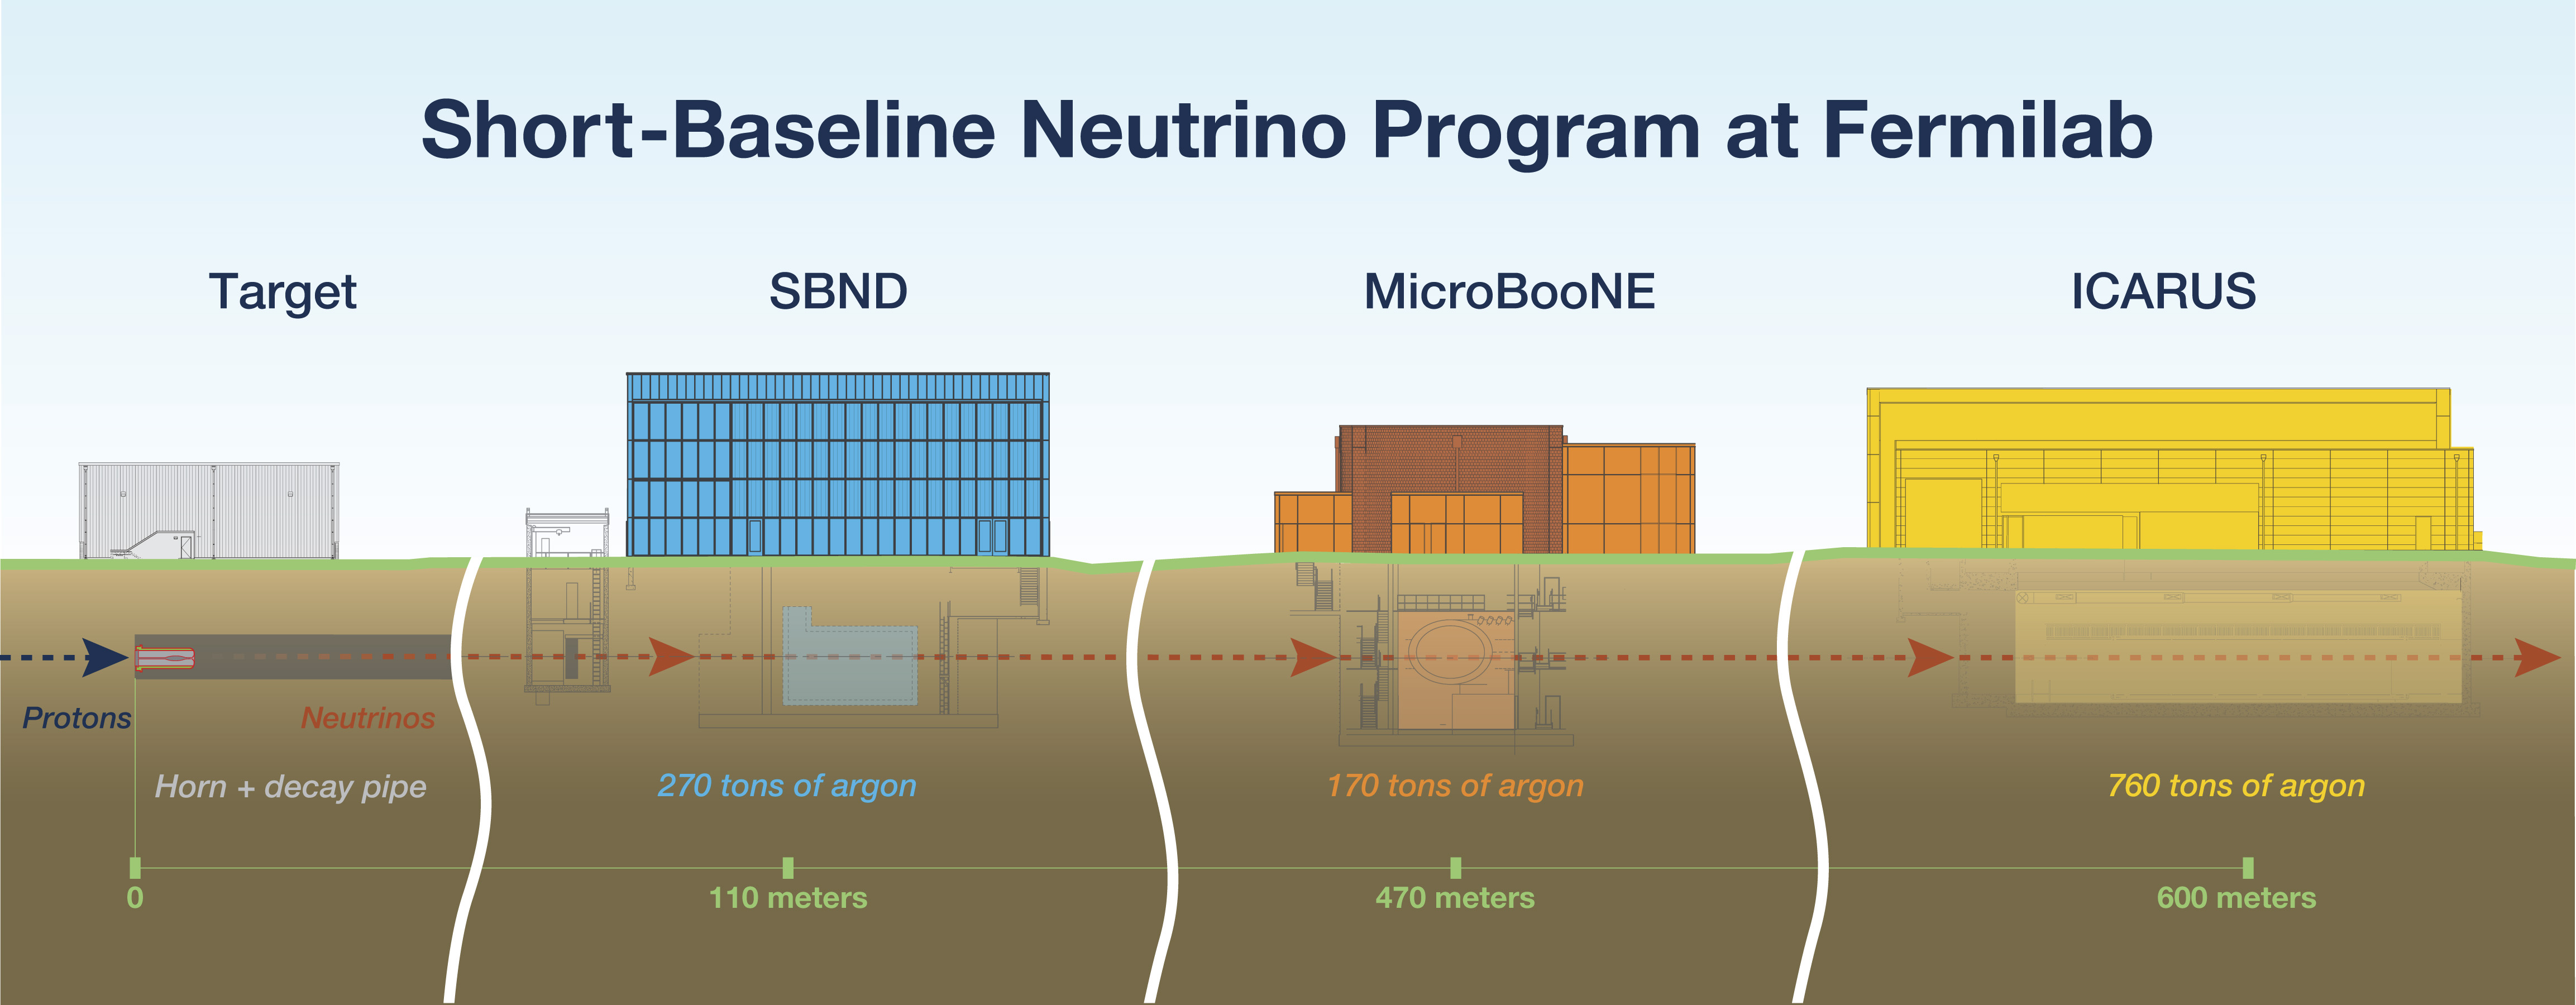
\includegraphics[width=\textwidth]{figures/introduction/sbn_program_diagram.jpg}
    \caption{Schematic diagram of the Short-Baseline Neutrino Program at Fermilab. The three detectors, SBND, MicroBooNE, and ICARUS T600, are located on-axis in the Booster Neutrino Beam. Image from Fermilab Visual Media Services.}
    \label{fig:sbn_program_diagram}
\end{figure}

The SBN Program, following the recommendations of P5, has four primary physics goals:

\begin{itemize}
    \item Conclusively resolve anomalies observed at short-baselines
    \item Characterize $\nu-Ar$ interactions
    \item Search for physics beyond the Standard Model
    \item Develop the LArTPC technology, software, and analysis tools for DUNE
\end{itemize}

\noindent
These four primary physics goals will each be described in detail below.

\paragraph*{Conclusively resolve anomalies observed at short-baselines}
The primary physics goal of the SBN Program is to conclusively resolve the short-baseline neutrino anomalies observed in the LSND and MiniBooNE experiments. The 3+1 minimal extension to the three-neutrino model provides effective oscillation probabilities for $\nu_\mu$ disappearance and $\nu_e$ appearance with which the SBN Program can explore the parameter space of the sterile neutrino hypothesis:

\begin{equation}
    \begin{aligned}
        P_{\nu_\mu \rightarrow \nu_\mu}^{3+1} & = 1 - 4 \left| U_{\mu 4} \right|^2 \left( 1 - \left| U_{\mu 4} \right|^2 \right) \sin^2{\frac{\Delta m_{41}^2L}{4E}}\\
        & \equiv 1 - \sin^2{2\theta_{\mu\mu}} \sin^2{\frac{\Delta m_{41}^2L}{4E}}
    \end{aligned}
    \label{eq:sbn_sterile_oscillation_probability_numu_disappearance}
\end{equation}

\begin{equation}
    \begin{aligned}
        P_{\nu_\mu \rightarrow \nu_e}^{3+1} & = 4 \left| U_{\mu 4} \right|^2 \left| U_{e 4} \right|^2 \sin^2{\frac{\Delta m_{41}^2L}{4E}}\\
        & \equiv \sin^2{2\theta_{\mu e}} \sin^2{\frac{\Delta m_{41}^2L}{4E}}
    \end{aligned}
    \label{eq:sbn_sterile_oscillation_probability_nue_appearance}
\end{equation}

\noindent
These two channels are the primary targets with the highest sensitivity due to the fact that the BNB is a predominately $\nu_\mu$ beam.

Electron neutrino candidates include intrinsic $\nu_e$ CC interactions as well as other beam-related mis-identified backgrounds. The SBN proposal \cite{Acciarri2015} chose a signal definition which requires the presence of a single electron shower with $E_e >$ 200 MeV and with an assumed identification efficiency of 80\% after restricting the candidate interaction vertices to the fiducial volume. The fiducial volume cut requires that the vertex of the interaction to be at least \qty[mode=text]{25}{cm} from the faces parallel to the beam, \qty[mode=text]{30}{cm} from the detector face upstream of the beam, and \qty[mode=text]{50}{cm} from the detector face downstream of the beam in order to maintain reconstruction fidelity. The 80\% efficiency target was estimated from hand-scanning simulated events and requires verification with automated reconstruction algorithms. 

In addition to the intrinsic $\nu_e$ CC interactions, there are several sources of background which can mimic the signal. Neutrinos interacting through NC channels may produce $\gamma$ showers above the 200 MeV shower cut, which can be mis-identified as electrons. For example, NC interactions which produce any number of $\pi^0$ in the final state or radiative resonant decays are sources of $\gamma$'s which can mimic the signal. Cuts on the number of reconstructed showers in an interaction along with conversion gap and $dE/dx$ cuts, which leverage the excellent spatial resolution and calorimetry of the LArTPC technology, can be used to suppress these backgrounds. 

Due to the relatively plentiful $\nu_\mu$ CC interactions, mis-reconstructed $\nu_\mu$ CC interactions with an electromagnetic shower can also fake a $\nu_e$ CC interaction. If the muon is not reconstructed or if the muon is mis-identified as a pion, the interaction may meet the signal definition. Tracks that are sufficiently long are almost entirely muons, so a cut on the track length can be used to suppress these backgrounds. Cosmogenic photons, either from a cosmic muon or produced in the atmospheric shower itself, may also create electromagnetic showers which can mimic the signal. Additional shielding in the form of a concrete overburden can reduce the rate of primary photons significantly, but does not eliminate the background imposed by primary cosmic muons. Instead, reconstruction cuts utilizing the interaction topology and timing information can be used to suppress these backgrounds, or robust estimation of the cosmic background through simulation or data can be used to characterize the background.

$\nu_\mu$ CC candidates are similarly selected assuming an 80\% reconstruction and identification efficiency after a fiducial volume cut has been applied (the same as described previously). This signal definition requires a muon in the interaction's final state. Beam-related backgrounds include NC charged pion production, as charged pions have a similar $dE/dx$ profile to muons and may therefore be mis-identified as muons. Charged pion tracks are typically quite short with most traveling less than half a meter in liquid argon, so a cut on the track length can be used to suppress these backgrounds. A minimum length of 50 cm for the candidate muon track was chosen in the SBN proposal to minimize these backgrounds.

Cosmogenic muons are a significant background for the $\nu_\mu$ disappearance search. Cosmogenic muons are most often out-of-time with respect to the beam window, so a cut on the timing of the interaction can be used as a first step to suppress these backgrounds. Furthermore, muons entering the detector can be tagged in a variety of ways. A muon which stops in the detector will have one end point at the detector boundary and exhibit a clear stopping signature in the form of a high rate of charge deposition at the opposite end of the track. The cosmic ray tagging system, which is a subsystem surrounding each of the three SBN detectors dedicated to tagging particles as they enter or exit the detector, can also be used to provide further cosmic background rejection. The combination of interaction timing and the requirement of an exiting or fully-contained track topology are sufficient to suppress the cosmic background to a manageable level.

Precise measurement of the energy of the neutrino interaction is essential for optimal sensitivity to neutrino oscillations and is contingent upon the calorimetric capabilities of the LArTPC technology. The reconstruction of the electron neutrino energy relies on the precise reconstruction of the resulting electromagnetic shower's energy. This is done by summing the charge deposited in the shower and converting it to an energy by accounting for the electronics gain, electron lifetime, and recombination effects. 

The reconstruction of the muon neutrino energy is dependant on whether the resulting muon track is fully contained or exiting. If the muon is fully contained, the energy can be estimated using the length of the muon track and the theoretically well-known rate of energy loss for muons in liquid argon. If the muon exits the volume, its energy must instead be estimated using the degree of scattering from Coulomb interactions present along the track. In order to attain sufficient energy resolution through multiple Coulomb scattering measurements, the SBN proposal places a 100 centimeter minimum length cut on exiting muon tracks.

\paragraph*{Characterize $\nu-\mathrm{Ar}$ interactions}
Precise neutrino-nucleus cross section measurements are a fundamental prerequisite for every neutrino oscillation experiment, especially for the future long-baseline experiment DUNE. The MeV-to-GeV neutrino energy range exposes the detectors of the SBN Program to a rich landscape of neutrino interactions on argon, ranging from the emission of a single nucleon to more complex final states with multiple pions or other hadrons. The LArTPC technology is particularly well suited to studying complex final states due to its high-resolution tracking and calorimetry capabilities. The slightly different detector geometries and locations of each detector in the SBN Program also enables important cross-checks of the neutrino-nucleus cross section measurements.

\paragraph*{Search for physics beyond the Standard Model}
The SBN Program is also well-positioned to search for physics beyond the Standard Model. Sterile neutrino decay is a mechanism which may explain the LSND and MiniBooNE anomalies \cite{Gninenko2009, Gninenko2012, Ballet2017}. In this process, an active neutrino interacts via a neutral-current process inside the detector and produces a heavy neutrino which subsequently decays into a light neutrino and a photon. The experimental signature is an interaction vertex in the upstream portion of the detector followed by a photon signal in the downstream region of the detector. The near detector has the advantage of higher statistics due to its location, while MicroBooNE and ICARUS have the advantage of a larger volumes for observing such a decay.

SBN will also be able to search for sub-GeV dark matter produced by the proton beam. Several recent studies have highlighted the sensitivity of the SBN experiments to light exotic new particles such as dark matter tridents \cite{Gouvea2019}, Higgs portal scalars \cite{Batell2019}, and elastically \cite{Buonocore2020} and inelastically \cite{Batell2021} scattering dark matter. This sensitivity to a wide range of new physics is enhanced by the location of off-axis location of MicroBooNE and ICARUS with respect to the higher-energy NuMI beam.

\paragraph*{Develop the LArTPC technology, software, and analysis tools for DUNE}
The scope and complexity of DUNE requires the development of new technologies and software tools that rise to the challenge of its physics goals. An important component of the viability of the LArTPC technology for DUNE is the scalability to the large detector volume required for the experiment while maintaining the high-resolution tracking and calorimetry capabilities. The SBN Program provides an opportunity to test similar cryostat, TPC, and PDS designs as those that will be used in DUNE.

The SBN Program requires an advanced suite of algorithms for signal processing, event reconstruction, and simulation, and analysis. These algorithms must account for detector effects such as the diffusion of the drifting ionization electrons, electron-ion recombination, impact of argon impurities on ionization charge loss, and electronics noise. Many of these effects can be characterized in the SBN detectors and will have immediate relevance for DUNE. The scalability of these algorithms to larger data volumes is also an important aspect of the development of the LArTPC technology for DUNE. Factorizing these algorithms into a common software framework will enable the sharing of tools and efficient development of new algorithms. The Liquid Argon Software (LArSoft) package is a realization of this detector-independent organization of common software tools for the simulation, reconstruction, and analysis of LArTPC data \cite{Snider2017}. This package is shared between the detectors of the SBN Program and DUNE, and much of the development of LArSoft is currently driven by SBN Program.

\subsection{The ICARUS Motivation}

The signal definitions chosen for the analysis presented here reflect both the goals of the ICARUS collaboration and the SBN Program more broadly. One of the near-term goals of the ICARUS collaboration involves a single-detector search for an eV-scale sterile neutrino, both as a contribution to the world knowledge of neutrino physics and as a demonstration of the capabilities of the ICARUS detector. Achieving this early physics result, before analysis tools have been fully optimized, has motivated the choice of relatively simple final states to minimize impacts to the analysis sensitivity from imperfect event reconstruction and detector modeling. 

The joint oscillation analysis of the SBN Program, as outlined in the SBN proposal \cite{Acciarri2015}, will involve an inclusive $\nu_\mu$ CC channel that encompasses a wide range of neutrino interaction topologies. This channel is therefore a key component of the SBN Program's physics reach, and the ICARUS collaboration has a strong interest in understanding the performance of the detector in terms of this signal selection.

\section{The ICARUS Machine-Learning Analysis Chain}
\label{chap:mlreco}
Traditionally, events in neutrino experiments based on the LArTPC technology are reconstructed using a set of algorithms that are tuned independently and rely on hand-engineered features. In recent years, machine learning (ML) has become a powerful tool in computer science, consistently breaking performance records in computer vision and natural language processing. The highly-visual nature of LArTPC data makes it a natural candidate for machine learning applications: the images of particles are easy to interpret by eye, but it is often hard to programmatically design algorithms to extract high-level features suitable for physics analyses. Moreover, the physics goals of the SBN Program assume high-purity and high-efficiency automatic selections that have so far remained out of reach of traditional pattern recognition techniques. This chapter describes the event reconstruction based on neural networks employed in the ICARUS experiment. Section \ref{sec:neural_networks} provides an overview of the different types of neural networks used in the ICARUS ML event reconstruction. An overview of the generators used to produce the training sample is provided in Section \ref{sec:training_datasets}. Section \ref{sec:ml_full_chain} describes the full ML chain used in the ICARUS ML event reconstruction, from the input data to the final output. Finally, Section \ref{sec:post_processing} describes the post-processing steps that are applied to the output of the neural networks to extract the final physics quantities.

\subsection{Neural Networks}
\label{sec:neural_networks}

Artificial neural networks can be described as a family of parameterized functional approximations that are inspired by the structure and function of the biological neural networks in the brain. The basic building block of a neural network is the artificial neuron, which is a simple computational unit that receives a signal from connected neurons and produces an output signal. The output signal is computed by some non-linear function of the weighted sum of the input signals. Typically, neurons are aggregated into layers and the layers are stacked to form a network. Signals travel from the input layer to the output layer, possibly traversing multiple intermediate ``hidden'' layers, with the output of one layer serving as the input to the next layer. A neural network is said to be ``deep'' if it has more than one hidden layer. Figure \ref{fig:neural_network} shows a schematic representation of a simple neural network with one hidden layer.

\begin{figure}
    \centering
    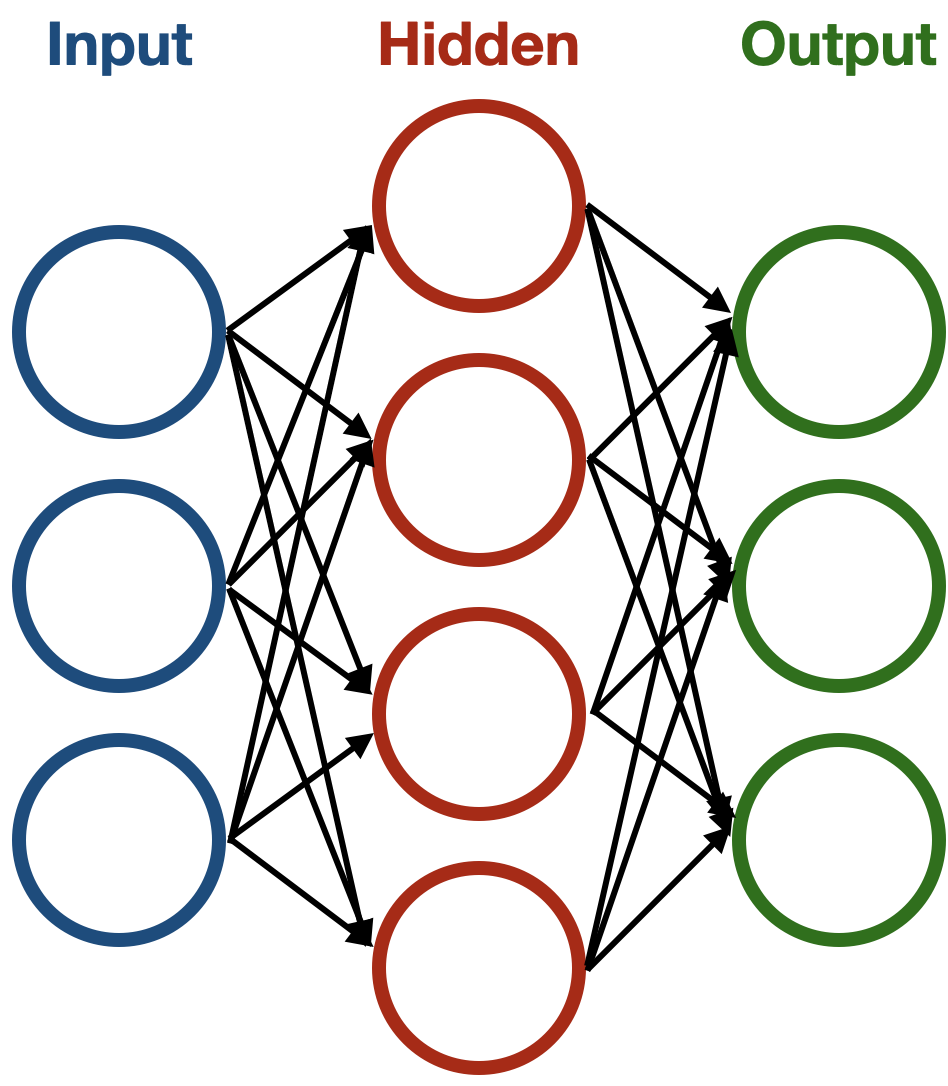
\includegraphics[width=0.5\textwidth]{figures/mlreco/neural_network.png}
    \caption{Schematic representation of a simple neural network with one hidden layer.}
    \label{fig:neural_network}
\end{figure}

The parameters of a neural network are typically optimized through gradient-based methods that serve to minimize a loss function. The loss function is a measure of the difference between the predicted output of the network and the target value. In a supervised learning setting, the target value is known and the network is trained to predict this value. This necessitates the use of labeled data, where the target value/category is known. For applications in neutrino physics, the role of a training sample is played by simulated data, where the truth information is known from the simulation. The trained network can then be applied to real data, where the target value is not known, to make predictions. 

\subsubsection{Convolutional Neural Networks}
\label{sec:cnn}

The convolutional neural network (CNN) is a type of neural network that is particularly well-suited for image recognition tasks. Compared to basic neural networks, CNNs make the additional assumption that most of the relevant information exists in a local neighborhood around the signal of interest. This is a natural description of LArTPC data, where the images of particles are highly structured and the local features are important for classification of particles/events. This requirement of sensitivity to local features motivates the use of convolutional layers in CNNs. A convolutional layer computes the dot product between its weights and a small region of the input data. The spatial extent of this region is called the receptive field of the neuron. This convolutional operation is iteratively moved across the entire input image producing an activation map, which may be stacked with other activation maps to obtain the output. Pooling layers are often used in conjunction with convolutional layers to reduce the spatial dimensions of the input data. This is done by aggregating the values of neighboring pixels in the input data with an operation such as max pooling or average pooling. A pooling layer also has the effect of expanding the receptive field as the aggregation method pulls in information from a larger region of the input data.

The restricted spatial extent of the convolutional layers allows CNNs to have fewer parameters than fully-connected networks, which would be computationally prohibitive for images of the size of LArTPC data. The use of shared weights in the convolutional layers also allows CNNs to learn translation-invariant features; that is, features that are detected regardless of their position in the image. This is particular desirable for LArTPC data where the position of the particle and the underlying space points in the detector is not relevant for the classification task.

\subsubsection{Graph Neural Networks}
\label{sec:gnn}

Graph neural networks (GNN) are a class of neural networks that are well-suited for datasets with a natural relational structure. The input data in a GNN is represented as a set of nodes and edges, where the nodes represent the entities of interest and the edges represent the relationships between the entities. The key design principle in GNNs is the use of message passing, a process by which the features of each node and edge are updated by aggregating the features of its neighbors. This is an iterative process performed across the entire graph, thus allowing the network to learn complex relationships between the nodes. Among all graph learning tasks, two are of particular relevance in this analysis:

\begin{itemize}
    \item \textbf{Node-learning tasks}: tasks that involve predicting the classification of a node. In the context of LArTPC data, an example is the classification of a particle as a muon or a primary particle coming out of the interaction vertex.
    \item \textbf{Edge-learning tasks}: tasks that involve predicting the classification of an edge. To relate to LArTPC data, an example is the classification of two particles being part of the same interaction, or of two shower fragments belonging to the same parent shower. 
\end{itemize}

\subsection{Training Datasets}
\label{sec:training_datasets}

The training of neural networks requires a labeled dataset, where the true output is known. In the context of LArTPC data, the labeled dataset is provided by the simulation of the detector response to a set of known particles. In order to avoid potential biases due to assumptions of particular physics models governing cosmic ray and neutrino generation, the reconstruction chain is trained using a set of simulated events produced by two physics-agnostic generators:

\begin{itemize}
    \item \textbf{Multi-Particle Vertex (MPV)}: this generator produces a set of up to $N$ particles originating from a common vertex. These particles include electrons, positrons, photons, muons, anti-muons, both negatively-charged and positively-charged pions, and protons.
    \item \textbf{Multi-Particle Rain (MPR)}: this generator produces a set of up to $M$ isolated particles. These particles include electrons, positrons, muons, anti-muons, and protons.
\end{itemize}

\noindent
The MPV generator is meant to emulate a pseudo-neutrino interaction with multiple particles emitted from a common vertex, whereas the MPR generator produces interactions that are similar to those produced by cosmic rays. For each particle, the generators are configured with a range of kinetic energies than can be assigned as well as a maximum particle multiplicity. The kinetic energy is drawn from a uniform distribution within the configurable range. The maximum particle multiplicity for a given vertex is enforced by only drawing particles of types that are not already at their preconfigured maximum.

The range of all parameters controlling the generation of training events is ideally a superset of the phase space observed in ICARUS data and Monte Carlo simulation. This is to avoid regions of phase space where performance of the reconstruction is worse due to relatively few encounters of events in this region of phase space in the training sample. For example, the reconstruction may struggle to correctly identify low-energy protons if the training sample does not have sufficiently high representation of low-energy protons. The particles generated by these generators are fed into the full detector simulation. This allows for the network to be trained on events that represent detector effects to the extent that they are modeled in the simulation.

\subsection{The ICARUS Machine Learning Analysis Chain}
\label{sec:ml_full_chain}

The Neutrino ML group at SLAC has developed an end-to-end, ML-based reconstruction chain for the ICARUS experiment. The chain consists of a hierarchical set of neural networks that are optimizable end-to-end. The two types of neural networks described in the preceding section are employed: CNNs and GNNs. The full chain is shown schematically in Figure \ref{fig:mlreco_schematic} and each stage is summarized in Table \ref{fig:mlreco_nn}. This section reviews each stage of the chain in order, starting from the voxel-level tasks and building up to the high-level particle- and interaction-level classifications. 

\begin{figure}
    \centering
    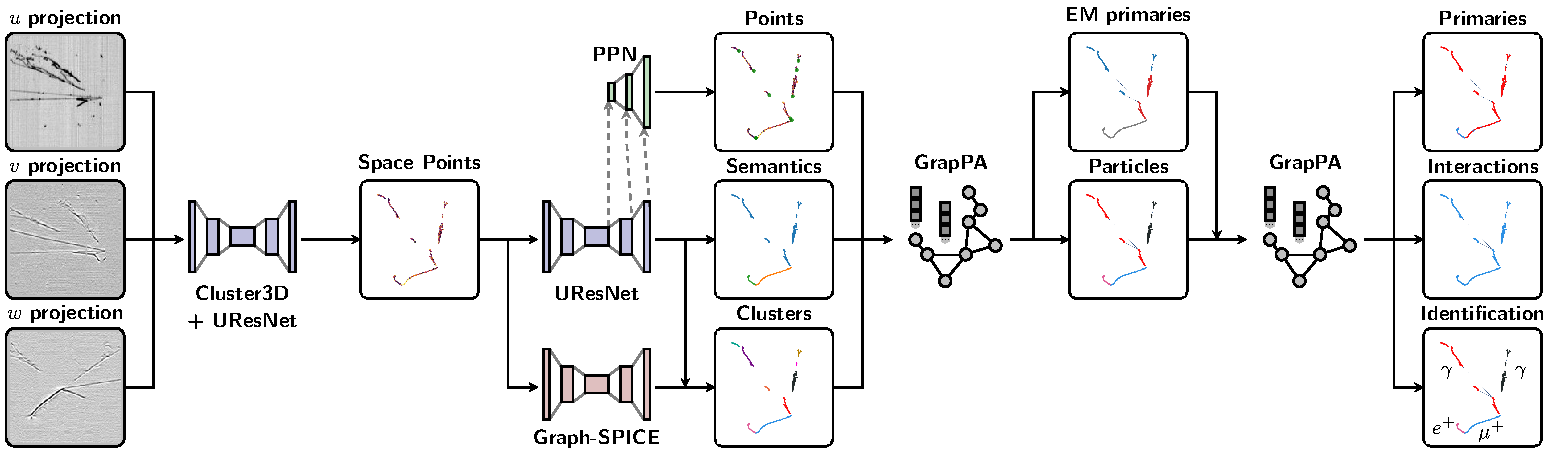
\includegraphics[width=0.95\textwidth]{figures/mlreco/mlreco_schematic.pdf}
    \caption{Schematic architecture of the end-to-end ML-based reconstruction chain used in the ICARUS experiment.}
    \label{fig:mlreco_schematic}
\end{figure}

\begin{table}
    \centering
    \caption{Summary of the neural networks used in the full ML event reconstruction chain in the ICARUS experiment.}
    \scalebox{0.8}{\begin{tabular}{ccccc}
    \toprule
    Stage & Type & Description \\
    \midrule
    UResNet Deghost & CNN & Classification of space points as reconstruction artifacts or real charge depositions \\
    UResNet & CNN & Semantic segmentation (voxel-level classification of activity) \\
    PPN & CNN & Prediction of start/end points of showers/tracks \\
    Graph-SPICE & CNN & Coarse clustering of space points into particle fragments \\
    GrapPA-Shower & GNN & Clustering of shower fragments into complete showers \\
    GrapPA-Track & GNN & Clustering of track fragments into complete tracks \\
    GrapPA-Interaction & GNN & Clustering of particles into complete interactions with PID and primary designation \\
    \bottomrule
\end{tabular}}
    \label{fig:mlreco_nn}
\end{table}

\subsubsection{Tomographic Reconstruction}
\label{sec:tomographic_reconstruction}

The reconstruction chain operates on a 3D set of points representing the charge depositions in the detector. Due to the detector's readout being intrinsically 2D, some additional processing is required to reconstruct the input 3D image. The process of reconstructing a higher-dimensional image from a set of lower-dimensional projections is generally known as tomographic reconstruction, and is a concept that is widely used in medical imaging. In the context of LArTPC data, the 3D space points are reconstructed from the hits found in each wire plane of the detector.

The algorithm that performs this task, called Cluster3D, is a part of the traditional reconstruction pipeline. Cluster3D considers all possible combinations of 2D hits and selects the ones with a consistent geometry that plausibly could have originated from the same 3D deposition. At a basic level, this means that the set of hits must originate from wires that intersect and they must have consistent hit times. Each match is assigned a score that factors in the distance between the hits in the time domain and the extent of each hit in time.

This algorithm considers both 3-hit combinations (triplets) and 2-hit combinations (doublets) to reconstruct the 3D space points. Inherent to the tomographic reconstruction process are ambiguities in the matching, resulting in the possibility of incorrect combinations. Space points formed by triplets are less likely to be an incorrect combination, though the inclusion of doublets increases the efficiency of reconstructing true 3D charge depositions. For the purposes of the ML reconstruction chain described here, the Cluster3D algorithm has been tuned to be highly efficient at the cost of a higher number of incorrect combinations.

These incorrect combinations are known as tomographic artifacts, or ``ghost points,'' and they are especially numerous for tracks parallel to the wire planes where the number of valid combinations of 2D hits is large. Figure \ref{fig:cluster3d} shows an example of a 2D event display of a neutrino interaction in the ICARUS detector and the corresponding 3D space points reconstructed by the Cluster3D algorithm. Of particular note is the presence of the ghost points in the 3D space points, which pose a challenge to visually identifying the true activity in the image. The first stage of the point classification task is to identify and remove these ghost points.

\begin{figure}
    \centering
    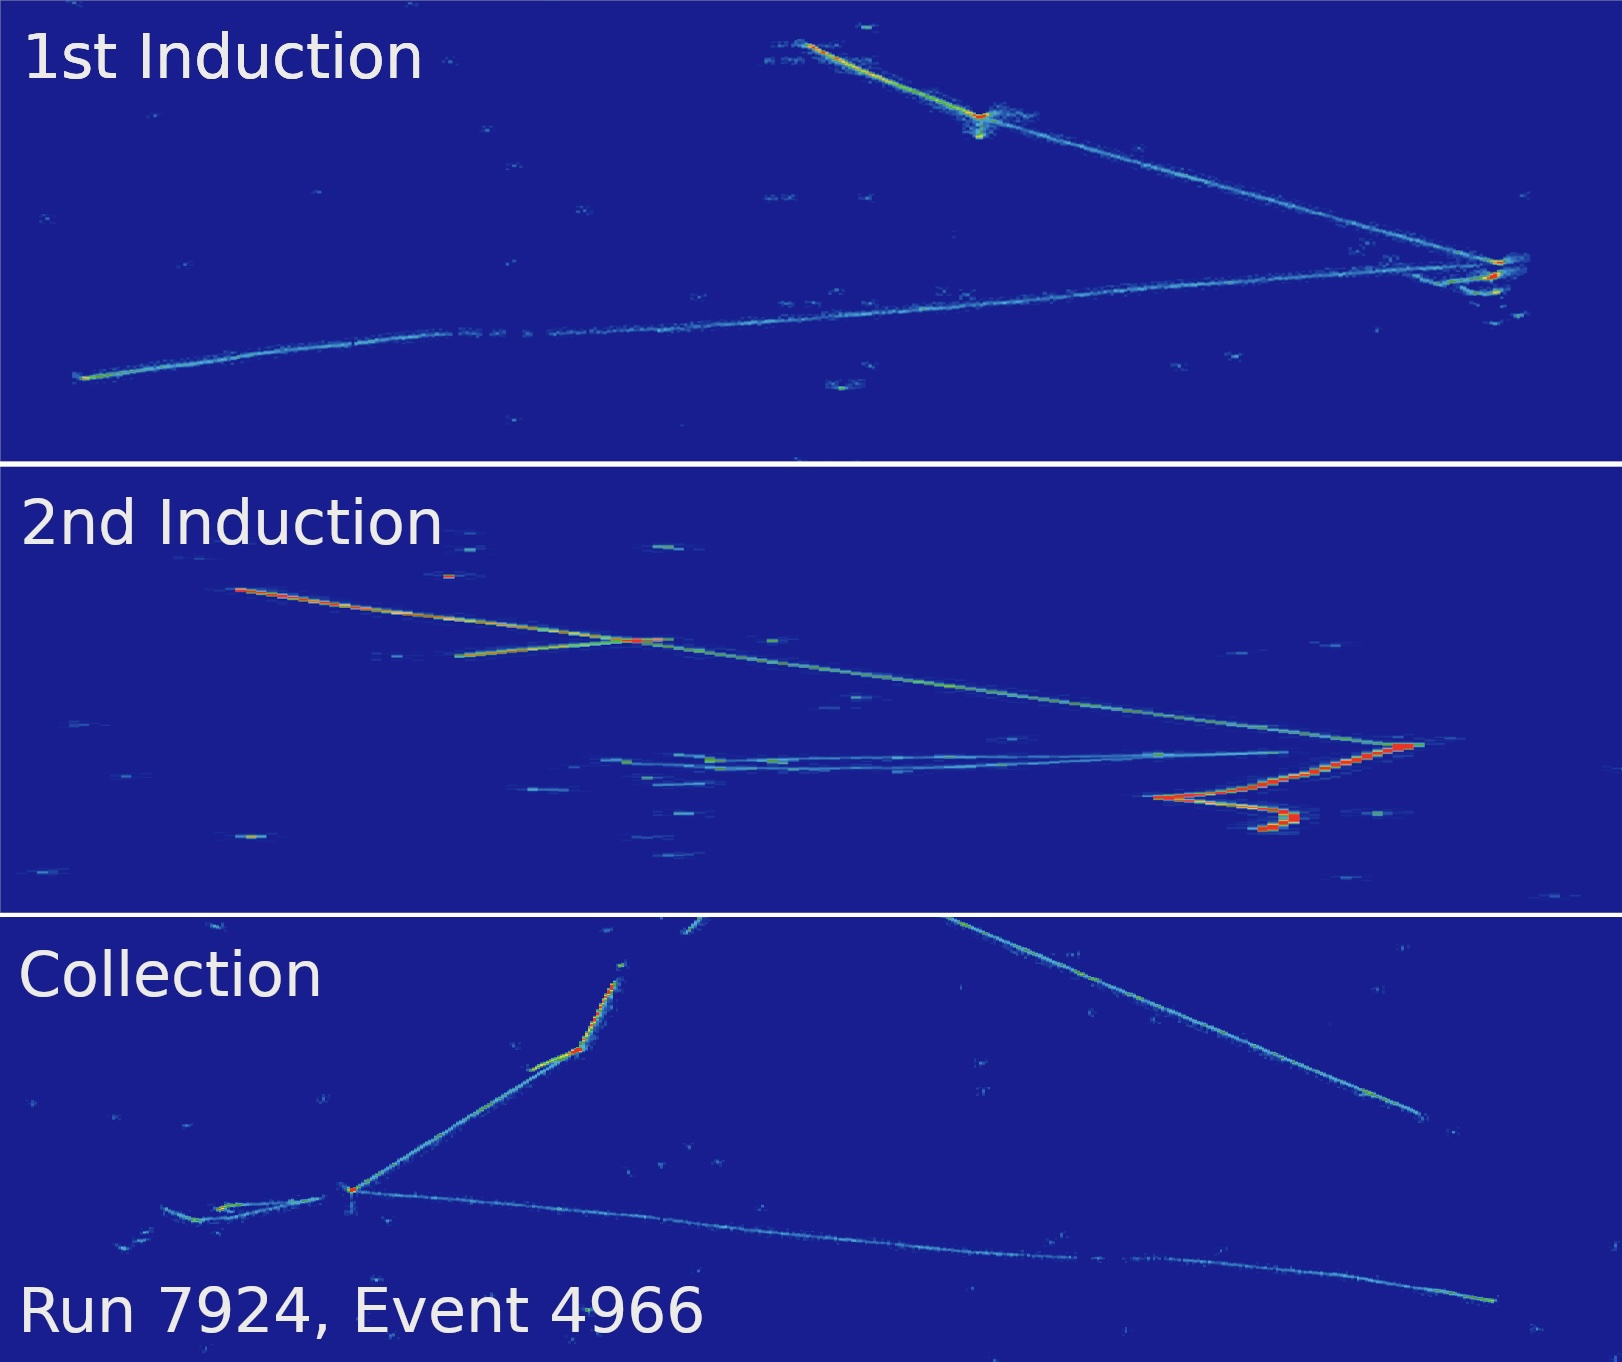
\includegraphics[width=0.45\textwidth]{figures/mlreco/mlreco_2d.jpg}
    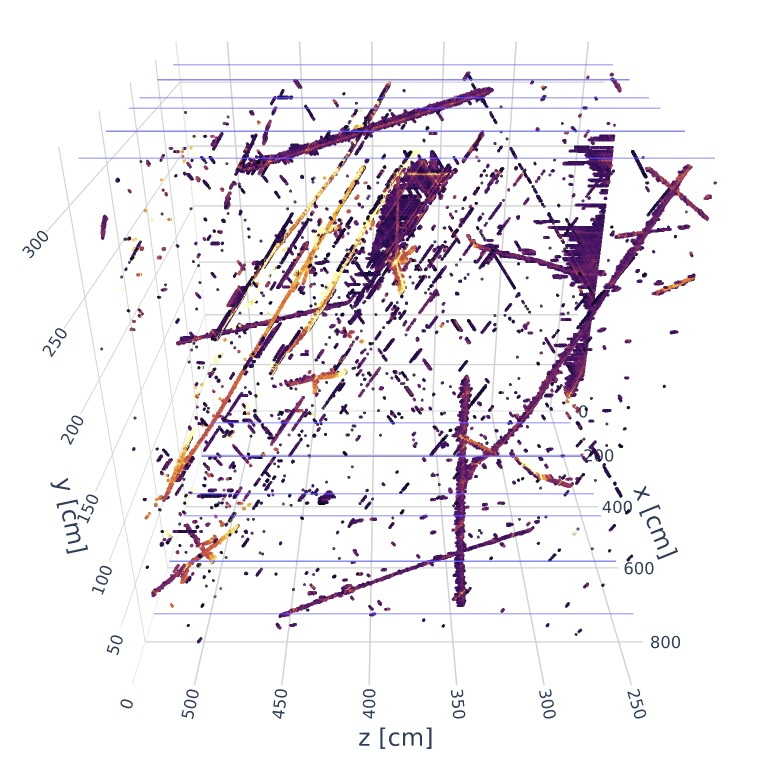
\includegraphics[width=0.45\textwidth]{figures/mlreco/mlreco_cluster3d.jpg}
    \caption{Example of a 2D event display of the same neutrino interaction in the ICARUS detector (left) and the corresponding 3D space points reconstructed by the Cluster3D algorithm (right). The image shown is a data event from Run 1.}
    \label{fig:cluster3d}
\end{figure}

\subsubsection{Point Classification}
\label{sec:point_classification}

\paragraph{Ghost point removal}
As a first step, the reconstruction is tasked with the removal of the tomographic artifacts, or ghost points, from Cluster3D (``deghosting''). The neural network used for this implements the U-ResNet architecture, which was first popularized due to its success in biomedical imaging \cite{Ronneberger2015}, to perform a binary classification of the space points, or semantic segmentation. Modifications were made to adapt U-ResNet to the sparse format of LArTPC data in contrast to regular images where each pixel contains information \cite{Domine2020b}. After deghosting, the reconstructed charge from Cluster3D is redistributed to enforce conservation of the overall charge. This is done by counting the number of times a given 2D hit is associated with a 3D space point and distributing the charge equally. The charge assigned to each space point is the average of the charge measured on each plane that contributed to the hit. An example image showing the 3D space points after the deghosting step is shown in Figure \ref{fig:deghosted}.

\begin{figure}
    \centering
    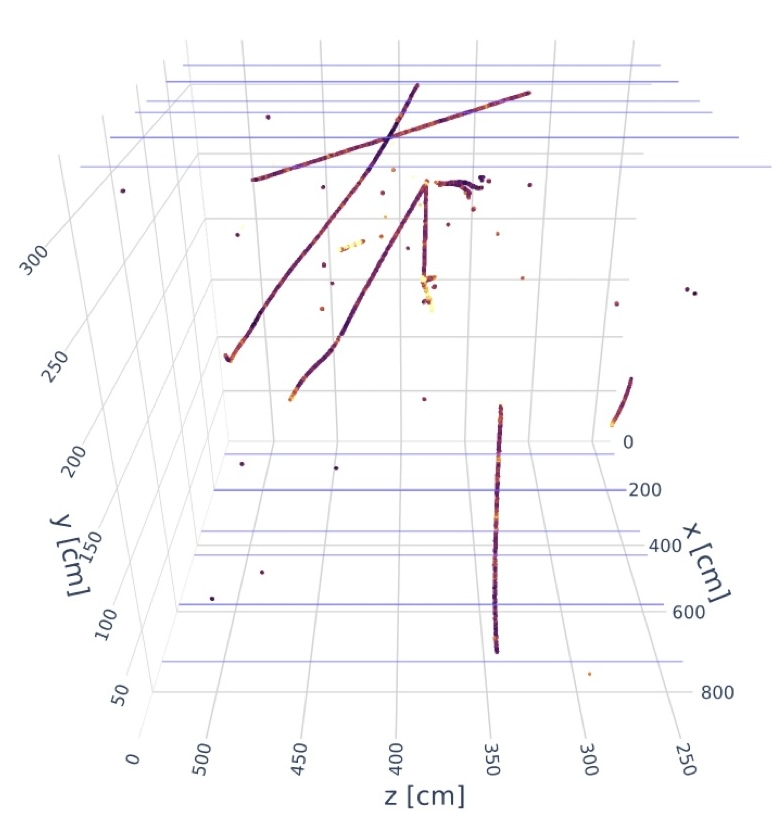
\includegraphics[width=0.6\textwidth]{figures/mlreco/mlreco_deghosted.jpg}
    \caption{Example of the 3D space points after the deghosting step. The image shown is a data event from Run 1 and the same as in Figure \ref{fig:cluster3d}.}
    \label{fig:deghosted}
\end{figure}

\paragraph{Semantic segmentation and point proposal network}
The next step in the point classification task is to classify the deghosted 3D space points into categories based on the type of parent activity that created them. The neural network used for this is a U-ResNet architecture, this time with five semantic classes of space points: Michel electron, delta ray, electromagnetic shower, track, and low-energy deposition. Each point is assigned a score for each class, and the class with the highest score is taken as the prediction. The semantic type of the space points is used in later stages of the reconstruction.

The point proposal network (PPN) is a neural network that is tasked to propose the 3D space points that are the initial and terminal points of track-like objects and the initial points of shower-like objects \cite{Domine2020a}. The PPN shares the same encoding backbone as the semantic segmentation network as shown schematically in Figure \ref{fig:mlreco_schematic}. The points of interest proposed by this network are valuable for high-level physics analyses (e.g.,\ particle start/end points and interaction vertex-finding) and are used in the clustering tasks in the later stages of the reconstruction. Figure \ref{fig:mlreco_points} shows the 3D space points colored by semantic class and the points proposed by the PPN.

\begin{figure}
    \centering
    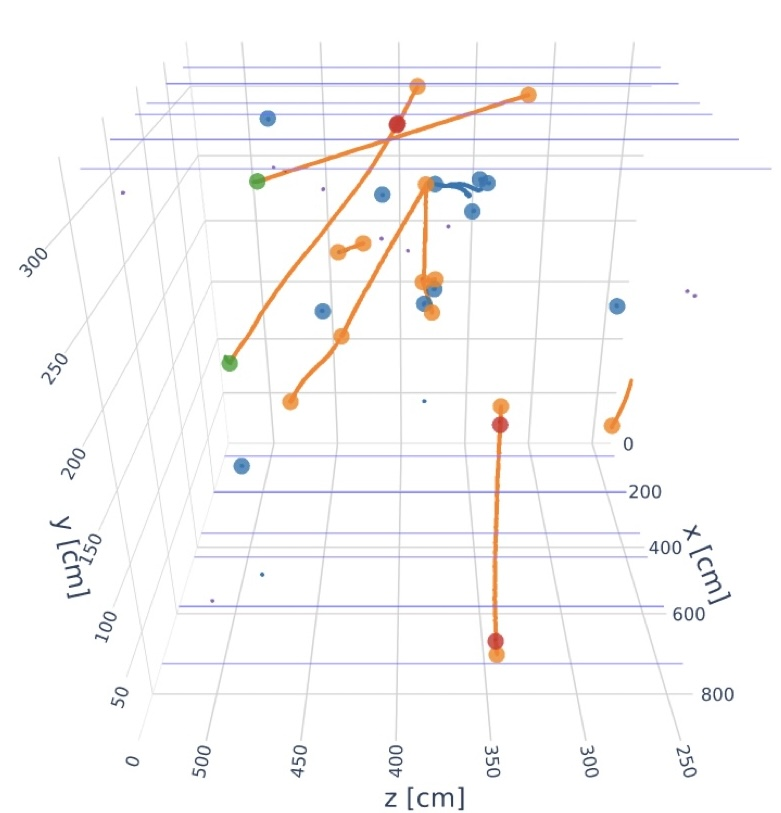
\includegraphics[width=0.45\textwidth]{figures/mlreco/mlreco_points.jpg}
    \caption{Example showing the 3D space points after the semantic segmentation and PPN stage. The space points are colored by the semantic type assigned by this stage (notably orange represents tracks, blue represents showers, green represents Michel electrons, and red represents delta rays). Also shown are the points of interest proposed by the PPN colored by the semantic class. The image shown is a data event from Run 1 and the same as in Figures \ref{fig:cluster3d} and \ref{fig:deghosted}.}
    \label{fig:mlreco_points}
\end{figure}

\paragraph{Point clustering}
The final step in the point classification task is to cluster the 3D space points in a set of points belonging to the same activity, i.e. track and shower fragments. This network, named Graph-SPICE, also uses a U-ResNet architecture and is tasked with learning an embedding of the space points in a higher-dimensional space where the points belonging to the same activity are close together. In this embedded space, the points belonging to the same semantic class are used to build a $k$-nearest neighbors graph, which connects the points that are close together. Each edge is given a score based on the feature vectors of the two points it connects and the edge is activated if the score is above a threshold. Space points are clustered into fragments by finding the connected components of the graph. The output of this stage is a set of point clusters, each representing a track or shower fragment. A paper detailing the Graph-SPICE network is in preparation.

\subsubsection{Formation of Particles and Interactions}
\label{sec:particle_interaction_reconstruction}

\paragraph{Particle instance clustering}
At this point in the reconstruction, groups of space points corresponding to particle fragments have been identified. The next step is to cluster these groups into particles. The neural network used for this task is a GNN that is tasked with a binary (on/off) edge classification, where an activated edge indicates that the two instances belong to the same particle. Two distinct GNNs are used for particle instance clustering: GrapPA-Track and GrapPA-Shower for tracks and showers, respectively. It is worth noting that these two GNNs have identical architecture and only differ in the tasks for which they have been trained. The details of the architecture of these GNNs are described in \cite{Drielsma2021}.

The node features in each GNN are mostly geometric quantities such as the particle fragment direction vector and the most-likely PPN point. Edge features are also geometry-based and include the distance between the two fragments. The initial state of the graph has activated edges for all node pairs up to a maximal distance. This limitation is motivated by both the computational cost associated with fully connecting an image in a detector as large as ICARUS and by physics concerns: beyond a certain length scale there cannot be legitimate connections. The result of these two GNNs is a set of complete particles of both the track and shower categories. Small gaps in tracks, for example due to track-breaking at the cathode, are expected to be resolved in this stage. The shower-clustering step also identifies the primary shower fragment that is used to identify the shower start point, a critical feature for the interaction-clustering step.

\paragraph{Interaction clustering}
The final stage of the event reconstruction is to cluster the particles into interactions, defined as a group of particles originating from the same vertex. Particles that are directly connected to the primary vertex are considered primary particles, meaning they are immediate products of the interaction, whereas other particles are labeled as secondaries. The clustering of particles into interactions is easily cast as an edge-classification task, where an activated edge indicates two particles belong to the same interaction. In addition to the interaction clustering, the network is also tasked with predicting for each node the particle type (photon, electron, muon, pion, or proton) and the primary/secondary label. The neural network used for this task is a GNN and is described extensively in \cite{Drielsma2021}. The architecture of this GNN differs from GrapPA-Track and GrapPA-Shower only in that it has more hidden features, which are useful for the extra tasks of particle identification (PID) and primary ID classification. The output of this stage is a full list of interactions in the event, each with a list of primary and secondary particles and their types.

\subsection{Post-Processing}
\label{sec:post_processing}

After the full chain of neural networks has been applied to the event, the output is a list of interactions with their associated particles. Each particle has been designated as a primary or secondary particle and has had a particle type assigned. In addition to this high-level set of information, a full physics analysis requires further information to be extracted from the event. This includes kinematic information such as the momentum and energy of the particles, as well as other geometric information such as the interaction vertex location. Association of interactions with the corresponding optical flash provides precise timing that can be leveraged in analyses. This information is extracted using traditional reconstruction algorithms that are well-established in the field of neutrino physics. 

\subsubsection{Kinematic Reconstruction}
\label{sec:kinematic_reconstruction}

The kinematic reconstruction of the particles in the event is performed using traditional reconstruction algorithms. Of relevance for the analysis presented here are the following reconstructed quantities:

\begin{itemize}
    \item \textbf{Particle direction reconstruction}: The direction of the particle at the start (tracks and showers) and end (tracks only) points is reconstructed using a principal component analysis (PCA) of the space points in the local neighborhood of the point. When combined with the kinetic energy of the particle, the momentum (direction and magnitude) can be reconstructed.
    \item \textbf{Calorimetric energy reconstruction}: The energy of the particle is reconstructed using the total charge deposited by the particle in the detector. The charge is converted to energy using an effective formula that accounts for the average amount of electron-ion recombination, the TPC electronics gain, the work function of liquid argon, the attenuation due to electron lifetime, and a scale factor that accounts for the missed shower fragments that have fallen below the detection threshold. This is most useful for showers, for which other methods of energy reconstruction are not available.
    \item \textbf{Track length reconstruction}: The length of the track is reconstructed by segmenting the track and summing the length of each segment along their respective principal axes. 
    \item \textbf{Range-based energy reconstruction}: The energy of the track is estimated using the well-known relationship between the kinetic energy of a particle and its range in a material according to the Bethe-Bloch formula. This relation is known as the Continuous Slowing Down Approximation (CSDA) and it is used to estimate the energy of the particle. This method assumes that the particle ranges out in the argon without nuclear interactions and that the track is fully contained in the detector.
    \item \textbf{Vertex reconstruction}: The interaction vertex is reconstructed as the point joining the start points of the primary particles in the interaction.
    \item \textbf{Fiducial volume}: The interaction vertex is used to determine if the interaction occurred within the fiducial volume of the detector. This is defined as the region \qty[mode=text]{25}{cm} from the edges of the detector in the $x$ and $y$ directions, \qty[mode=text]{30}{cm} from the upstream edge in the $z$ direction, and \qty[mode=text]{50}{cm} from the downstream edge in the $z$ direction. These numbers were assumed in the SBN proposal \cite{Acciarri2015} and are chosen to avoid reconstruction inefficiencies near the edges of the detector (e.g.\ exiting particles that are not seen).
    \item \textbf{Containment}: The containment of the particles in the detector is determined by requiring that all the space points of the particle are at least \qty[mode=text]{5}{cm} from the edges of the detector. At the interaction level, the interaction is considered contained if all of the particles that comprise it are contained. The containment cut also applies the constraint that the space points must be in the same TPC that created them; out-of-time tracks may be reconstructed partially in the wrong TPC and therefore be removed by this cut. The value of \qty[mode=text]{5}{cm} was chosen based on the expected magnitude of space charge effects in the detector, which tends to displace space points away from the detector boundaries.
\end{itemize}

\subsubsection{Optical Flash Association}
\label{sec:optical_flash_association}

The optical flash is a prompt signal in the PMTs associated with the scintillation light produced by the neutrino interaction in the detector. As part of the standard reconstruction chain, the optical flash is formed from optical hits, which themselves are reconstructed from the PMT waveforms. This flash object can be thought of as a set of optical hits each with a well-defined position, time, and photoelectron count. The job of the flash association algorithm is to leverage these characteristics and match them to the interactions in the event that are imaged by the TPC through detection of ionization charge signals.

The tool used for flash association is a package originally developed for MicroBooNE called OpT0Finder. OpT0Finder employs a likelihood-based approach to match the optical flash to charge activity associated with an interaction in the event. For each interaction, as defined by the upstream ML reconstruction, the algorithm calculates an allowed range of $x$ offsets that are allowed by the geometry. This reflects our inability to know beforehand the exact time of the interaction. For each of these allowable positions\footnote{This is not actually a brute-force algorithm, but rather an optimization algorithm that profiles across the drift direction.}, the algorithm calculates a hypothesis flash based on the expected light yield of the interaction, the distribution of the ionization charge in the interaction, and the position of the PMTs in the detector. The hypothesis flash and the observed flash each have a likelihood computed using a joint probability distribution of the photoelectron count in each PMT given the $x$ position of the flash. Maximizing the likelihood between the two allows the assignment of a score to each potential interaction-flash pair. 

A matching algorithm then selects the best pairings based on the scores while simultaneously skipping pairs with an already matched flash or interaction. The result of this association process is the assignment of a time stamp to each interaction which was successfully matched to a flash. This time stamp can be used to precisely tag an interaction as being in-time or out-of-time with respect to the beam spill, and therefore can be leveraged as a tool for cosmic rejection.

\section{Muon Neutrino Interaction Selection and Performance}
\label{chap:neutrino_selection}
This chapter provides an overview of the chosen signal definitions for the analysis presented here. The signal definitions are chosen to reflect the goals of the ICARUS collaboration and the SBN Program, and are designed to be simple and robust to the imperfections in the reconstruction and simulation. An overview of the signal channels and the selections are given in Section \ref{sec:neutrino_signal_definitions}. The chapter also presents the variables used to characterize the performance of the selections (Section \ref{sec:variables_of_interest}) as well as the performance of the selections on simulation (Section \ref{sec:selection_performance}).

\subsection{Neutrino Signal Definitions and Selections}
\label{sec:neutrino_signal_definitions}

\subsubsection{Signal Channels}
\label{sec:signal_channels}

Three signal definitions are chosen to accomplish the goals described above: a $\nu_\mu$ CC 1$\mu$1$p$ channel, a $\nu_\mu$ CC 1$\mu$N$p$ channel, and a $\nu_\mu$ CC inclusive channel. In common to all three of these signal channels are a few key features:

\begin{itemize}
    \item \textbf{Containment}: The entirety of the interaction is required to be contained within a volume that is defined as \qty[mode=text]{5}{cm} from the edges of the detector in all three dimensions. This requirement ensures that the range-based energy reconstruction, which has significantly better resolution than other methods, can be applied to tracks in the final state.
    \item \textbf{Fiducial Volume}: The interaction vertex must be located within the fiducial volume of the detector, which is defined as the region \qty[mode=text]{25}{cm} from the edges of the detector in the $x$ and $y$ directions, \qty[mode=text]{30}{cm} from the upstream edge in the $z$ direction, and \qty[mode=text]{50}{cm} from the downstream edge in the $z$ direction. This requirement is motivated by the desire to avoid the reconstruction inefficiencies and biases that can arise near the edges of the detector.
    \item \textbf{Single Muon}: Each signal definition requires the presence of a single primary muon in the final state. This muon is required to have a length of at least \qty[mode=text]{50}{cm}, principally to reduce the contamination from NC interactions with a pion in the final state. This length threshold is also consistent with the proposed selection in the SBN proposal.
    \item \textbf{Proton Threshold}: Protons are required to be primary particles and to have deposited at least \qty[mode=text]{50}{MeV} of energy to count towards the final state of the interaction. This threshold is chosen to ensure that the proton is sufficiently long to be reconstructed as a track and to ensure that the proton is energetic enough to be well-separated from the muon in the final state. Interactions with one proton above threshold and one proton below threshold are classified as 1$\mu$1$p$ final states under this definition.
    \item \textbf{Other Particles}: The final state may contain additional protons, pions, and showers. These particles are required to be primary particles and to have deposited at least \qty[mode=text]{25}{MeV} of energy to be counted towards the final state of the interaction. This threshold is chosen to ensure that the particles are sufficiently energetic to be visible in the final state.
\end{itemize}

The 1$\mu$1$p$ channel requires exactly one proton above threshold in addition to the muon, while the 1$\mu$N$p$ channel requires \text{at least} one proton above threshold in addition to the muon. The $\nu_\mu$ CC inclusive channel requires only the presence of a single muon in the final state and any number of other final state particles above threshold. The structuring of these signal definitions means that the 1$\mu$1$p$ channel is a subset of the 1$\mu$N$p$ channel, which is in turn a subset of the $\nu_\mu$ CC inclusive channel. 

While the 1$\mu$1$p$ and 1$\mu$N$p$ channels are inherently more statistically limited than the $\nu_\mu$ CC inclusive channel, they provide simple final states that are well-suited to the early stages of the ICARUS physics program. The energy reconstruction for these two channels is also more precise due to the simple final state, which may be beneficial for neutrino oscillation physics measurements. Additionally, these final states are particularly low in cosmic background, especially in combination with the containment requirement. In contrast, the $\nu_\mu$ CC inclusive channel is more statistically powerful and provides a more complete picture of the detector performance due to the wider range of neutrino interaction topologies. Final states in this channel may also contain showers, the precise reconstruction of which is of significant importance for any future oscillation analysis.

\subsubsection{Additional Selections}
\label{sec:additional_selections}

In addition to the requirements described above, the following selections are applied to the reconstructed interactions to further reduce the background and improve the purity of the selected samples:

\paragraph{Flash Time:}
Each interaction is required to be matched with an optical flash detected by the PMTs that is consistent with the time of the neutrino beam spill. The association of the interaction with the flash is performed with OpT0Finder, as described in Section \ref{sec:post_processing}. This analysis targets neutrinos from the BNB, which has a spill length of \qty[mode=text]{1.6}{us}. The requirement that interactions be associated with a flash in-time with the beam provides significant background rejection of cosmic-induced interactions that are not in-time with the beam. This cut is not expected to provide significant background rejection for cosmic-induced interactions that are in-time with the beam and trigger the detector readout.

\paragraph{CRT Veto:}
Each event has a collection of PMT flashes and CRT hits. As part of the standard reconstruction chain, a matching algorithm is run to associate the CRT hits with the PMT flashes using timing information. This analysis makes use of this association by requiring that selected events have at least one flash within the beam spill window that is not matched to a CRT hit. This requirement strongly suppresses cosmic-induced interactions, and is complementary to the flash time cut discussed above in that it rejects many of the cosmic-induced interactions that are in-time with the beam. This veto uses only the Top and Side CRT subsystems, as the Bottom CRT subsystem was not fully commissioned prior to the data used in this analysis.

\subsubsection{Neutrino Sample Composition}
\label{sec:neutrino_sample_composition}
The primary sample used in this analysis to set the central value expectation for the selections is a sample of simulated neutrino interactions produced according to the predicted BNB flux and overlayed with the expected out-of-time cosmic flux. The size of this sample is $2.68 \times 10^{20}$ POT, which is more than a factor of ten larger than the recorded dataset of $1.92 \times 10^{19}$ POT for this analysis. The statistical uncertainty of this larger simulated sample is negligible for the analysis presented here. It is worth noting that the neutrinos in this sample are required to interact in the active volume of the detector. The contribution to the expected event rates from neutrinos that interact outside of the active volume is expected to be negligible and thus is not included in this analysis.

Most of the triggered events in data are due to cosmic muons in-time with the beam, which are not present in the simulated neutrino sample. Rather than attempting to model the cosmic background with a simulated dataset, the cosmic background is estimated using the off-beam dataset. This method is expected to provide a more accurate estimate of the cosmic background than a simulated dataset, which would be subject to uncertainties in the cosmic flux and the detector response to cosmic-induced interactions. The scaling of the off-beam dataset to the on-beam dataset is based on matching the number of opened trigger gates in the two datasets. Though the number of opened trigger gates is one-to-one, and therefore the number of on-beam and off-beam events is near equal, there is a limited statistical penalty due to both the smallness of the background and the ability to use the entire off-beam dataset rather than the 10\% that is used for the on-beam dataset due to blinding considerations. The on-beam dataset used in this analysis will be described in more detail in Chapter \ref{chap:data_mc_comparisons} and the uncertainty associated with the data-driven cosmic background estimate will be assessed in Chapter \ref{chap:systematics}.

\subsection{Variables of Interest}
\label{sec:variables_of_interest}

This section presents an overview of the variables used to characterize the performance of the three selections described in the preceding section. The variables are divided into three categories: interaction kinematic variables, kinematic imbalance variables, and PID variables. The distributions of these variables can be used to validate the performance of the selections and to identify potential sources of bias or inefficiency in the reconstruction and simulation. In each of the following plots, the distributions are made with truth information to show the true distributions of these variables for each of the signal channels prior to any reconstruction or selection effects. The distributions are also scaled to the recorded dataset of $1.92 \times 10^{19}$ POT to show the predicted event rates.

\subsubsection{Interaction Kinematic Variables}
\label{sec:interaction_kinematic_variables}
These variables reflect the kinematics of the neutrino interaction and the final state particles. The total energy of the interaction is a key variable for understanding the energy of the parent neutrino, while the kinematics of the final state particles can provide information about the nature of the interaction and the performance of the reconstruction. The total energy of the interaction is a necessary input to oscillation analyses. Additionally, these variables are often used in cross section measurements to probe the underlying physics of neutrino interactions. For the chosen signal definitions, there is always a single primary muon and there may be additional primary protons, pions, and showers above the energy threshold of the signal definition. 

\paragraph{Muon Kinetic Energy ($\mathbf{T_\mu}$):}
The kinetic energy of the muon as calculated using the Continuous Slowing Down Approximation (CSDA) \cite{Zyla2020} to relate the muon track length (range) to its kinetic energy. This method is typically known as ``range-based'' kinetic energy reconstruction.

\paragraph{Leading Proton Kinetic Energy ($\mathbf{T_p}$):}
The kinetic energy of the most energetic primary proton as calculated using the CSDA to relate the proton track length (range) to its energy.
    
\begin{figure}[!htb]
    \centering
    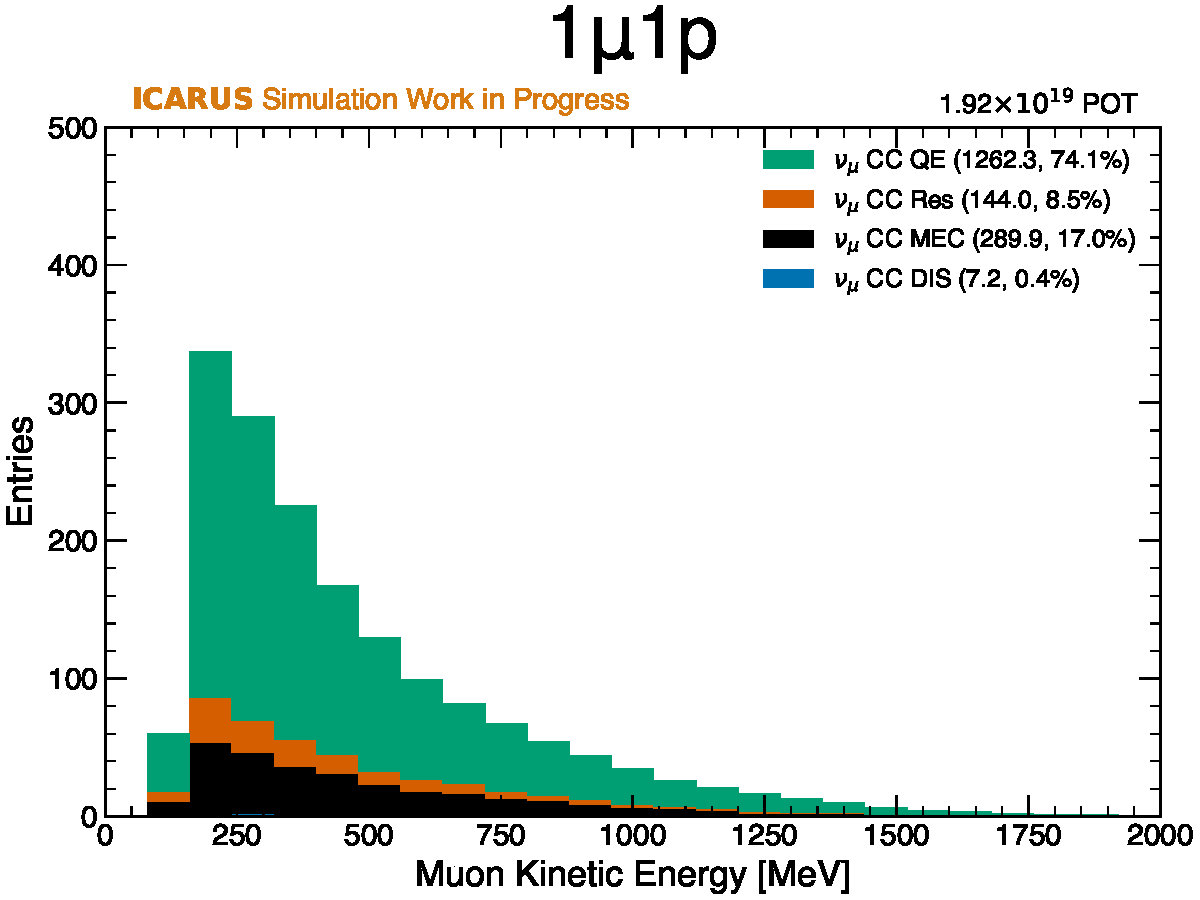
\includegraphics[width=0.48\textwidth]{figures/neutrino_selection/signal_hist1d_1mu1p_muon_ke.pdf}
    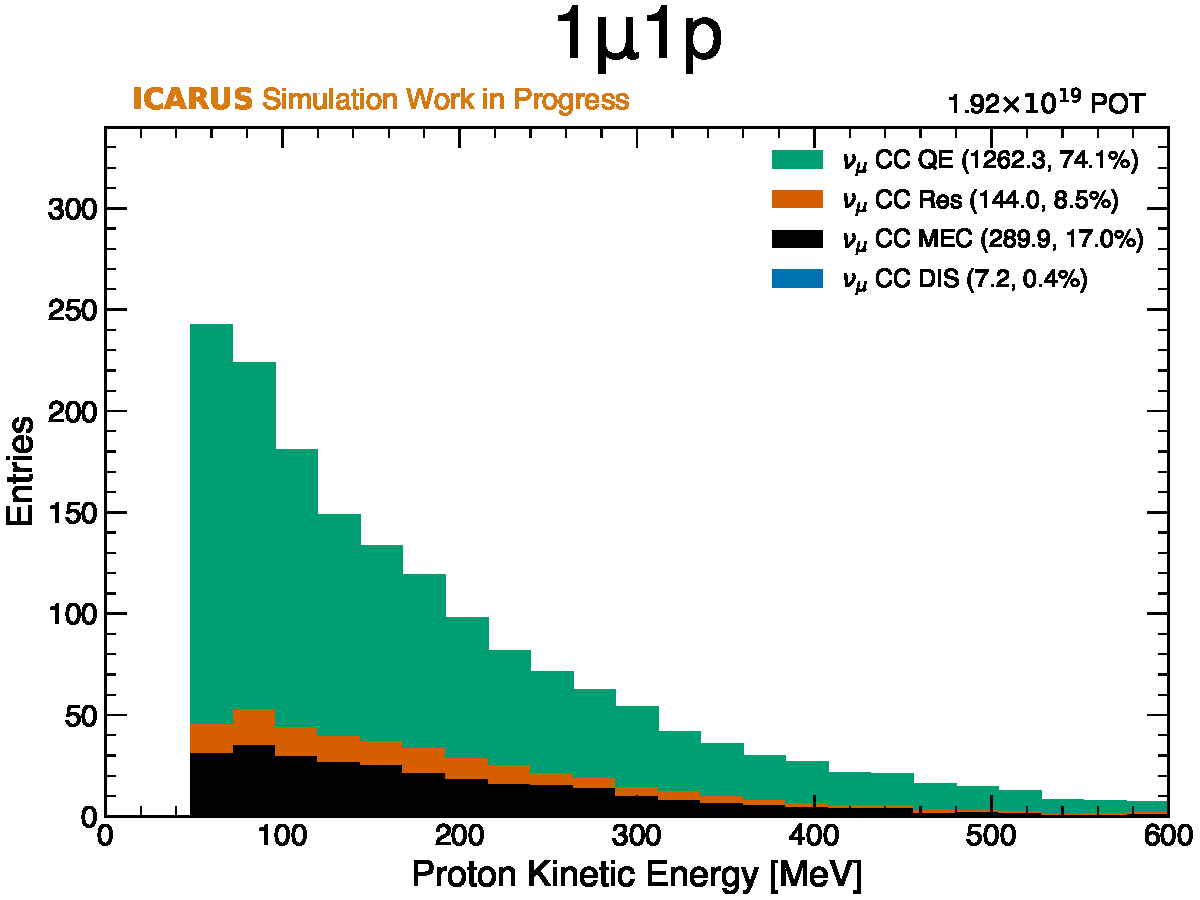
\includegraphics[width=0.48\textwidth]{figures/neutrino_selection/signal_hist1d_1mu1p_proton_ke.pdf}
    \\
    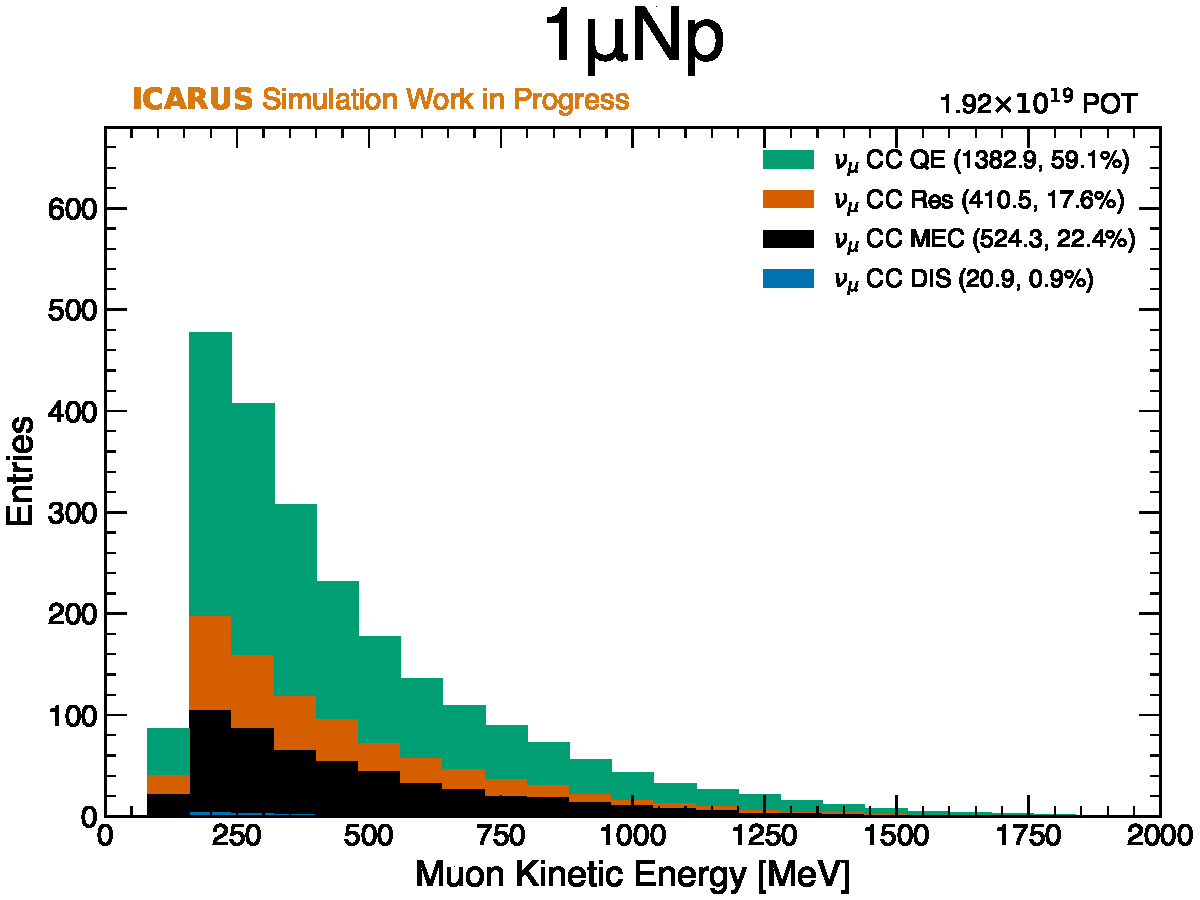
\includegraphics[width=0.48\textwidth]{figures/neutrino_selection/signal_hist1d_1muNp_muon_ke.pdf}
    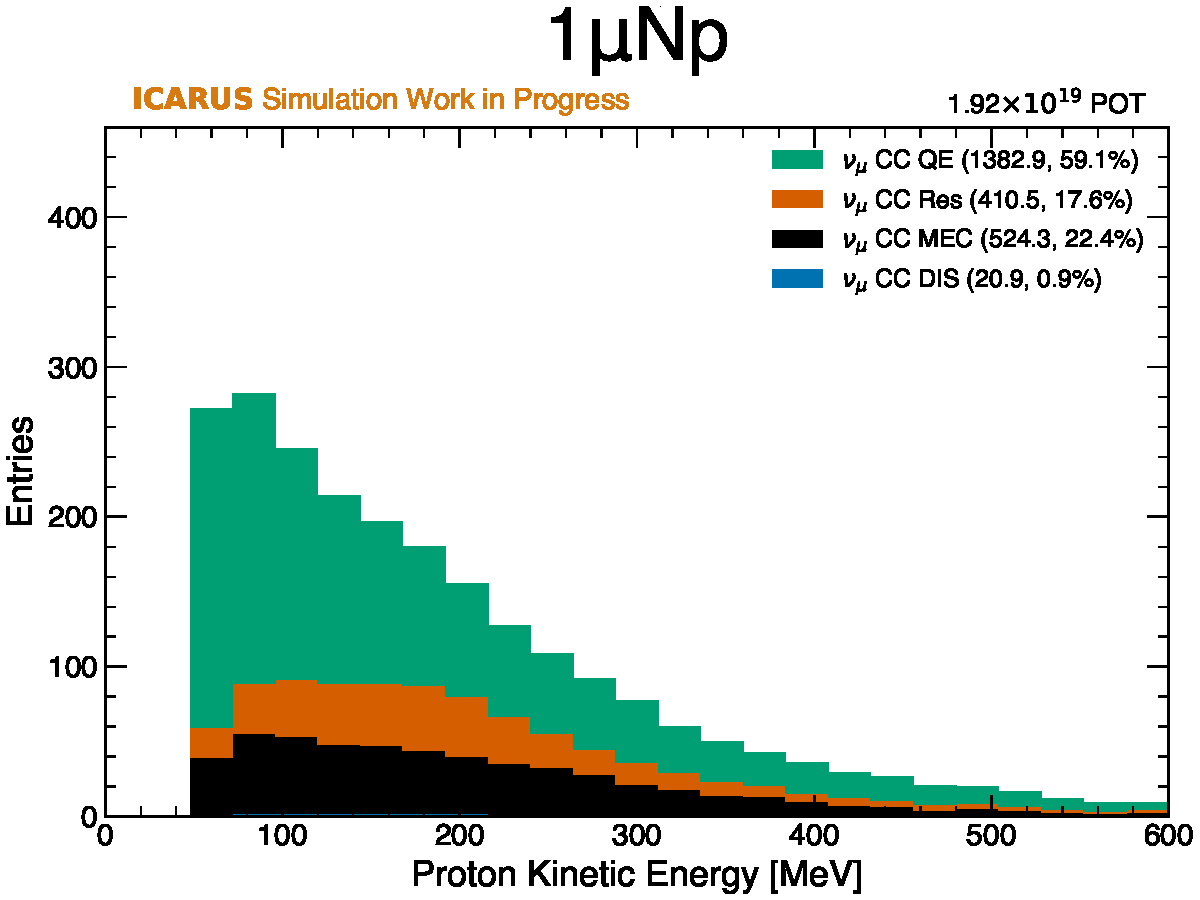
\includegraphics[width=0.48\textwidth]{figures/neutrino_selection/signal_hist1d_1muNp_proton_ke.pdf}
    \\
    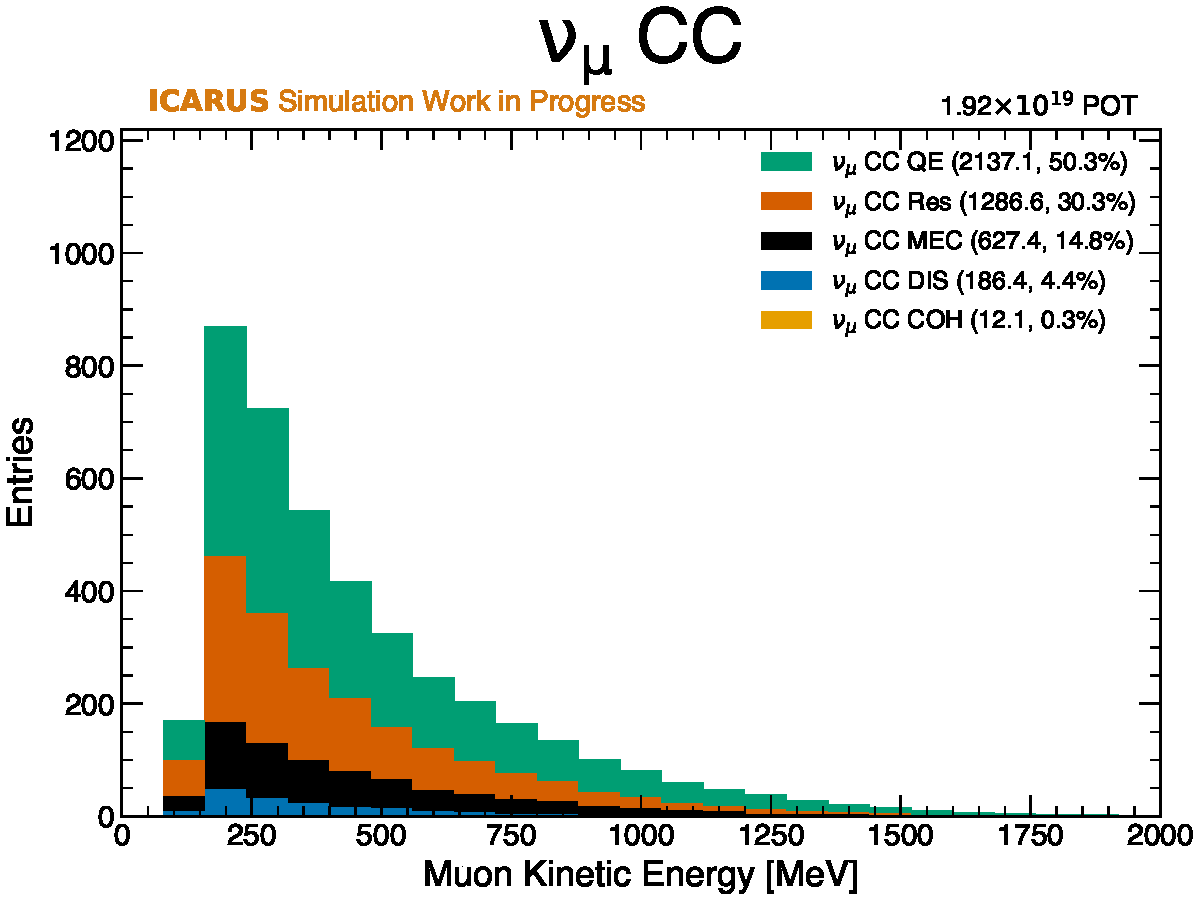
\includegraphics[width=0.48\textwidth]{figures/neutrino_selection/signal_hist1d_1muX_muon_ke.pdf}
    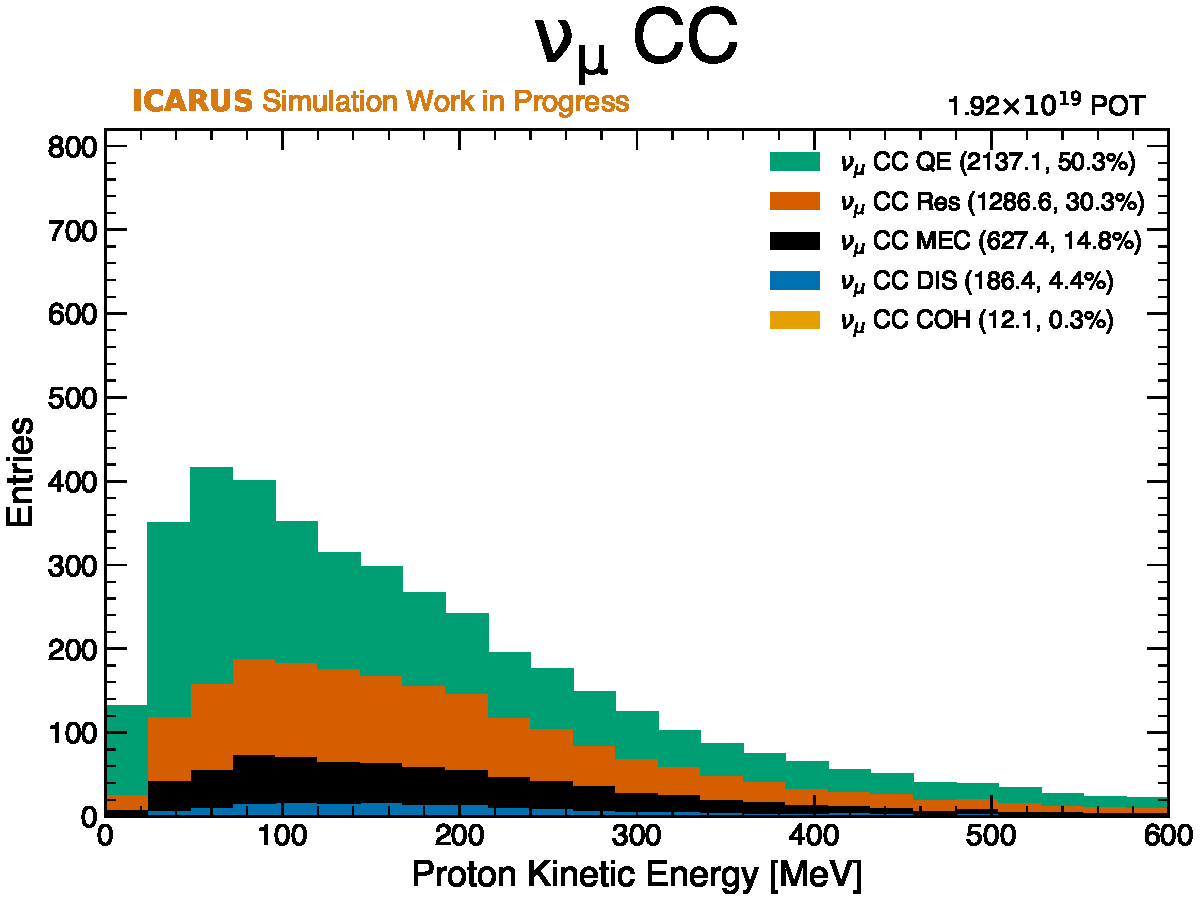
\includegraphics[width=0.48\textwidth]{figures/neutrino_selection/signal_hist1d_1muX_proton_ke.pdf}
    \caption{Kinetic energy of the muon (left) and the most energetic proton (right) for each of the three signal channels: from top to bottom $\mathrm{1\mu 1p}$, $\mathrm{1\mu Np}$, and $\nu_\mu$ CC inclusive.}
    \label{fig:muon_proton_ke}
\end{figure}

\paragraph{Interaction Visible Energy ($\mathbf{E_{vis}}$):}
The best estimate of energy deposited in the detector by the neutrino interaction. The energy deposited by primary showers are estimated by summing the deposited charge and converting it to energy using an effective constant that accounts for electron-ion recombination and shower clustering efficiency. Primary muon, pion, and proton energies are estimated using the CSDA to relate the track length to the energy deposited. In addition to the kinetic energies of the particles, the mass of the particle is also included in the energy calculation for the muon and pion, which are created rather than ejected during the interaction. Neutrons leading to recoiling protons are not currently included in the energy calculation as they are classified as secondaries and only primary particles are included for now. The interaction visible energy is therefore calculated as:
\begin{equation}
    E_{\text{vis}} = \sum_{\mathrm{Showers}} E^{calo}_{\mathrm{shower}} + \sum_{\mathrm{Muons}} E^{range}_{\mathrm{muon}} + \sum_{\mathrm{Pions}} E^{range}_{\mathrm{pion}} + \sum_{\mathrm{Protons}} T^{range}_{\mathrm{proton}}
\end{equation}

\begin{figure}[!htb]
    \centering
    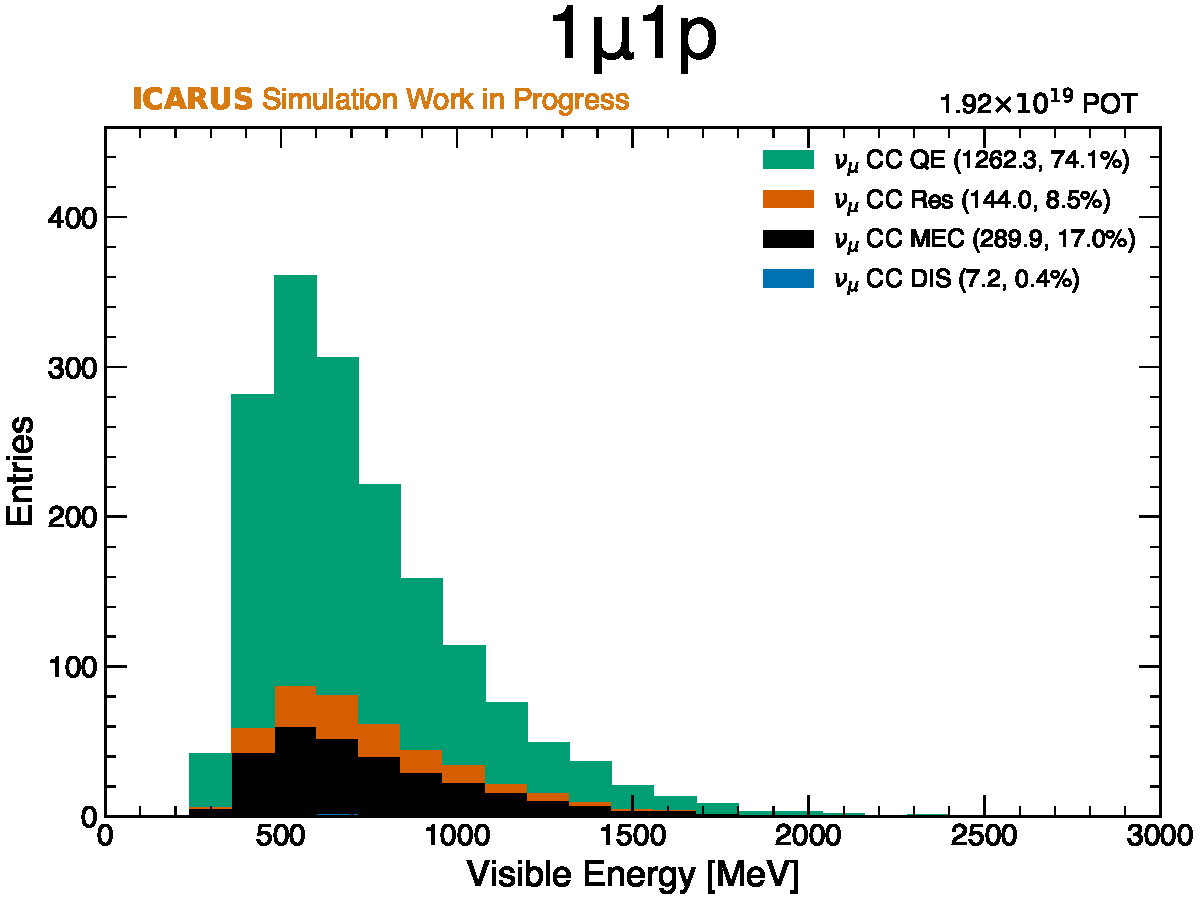
\includegraphics[width=0.48\textwidth]{figures/neutrino_selection/signal_hist1d_1mu1p_visible_energy.pdf}\\
    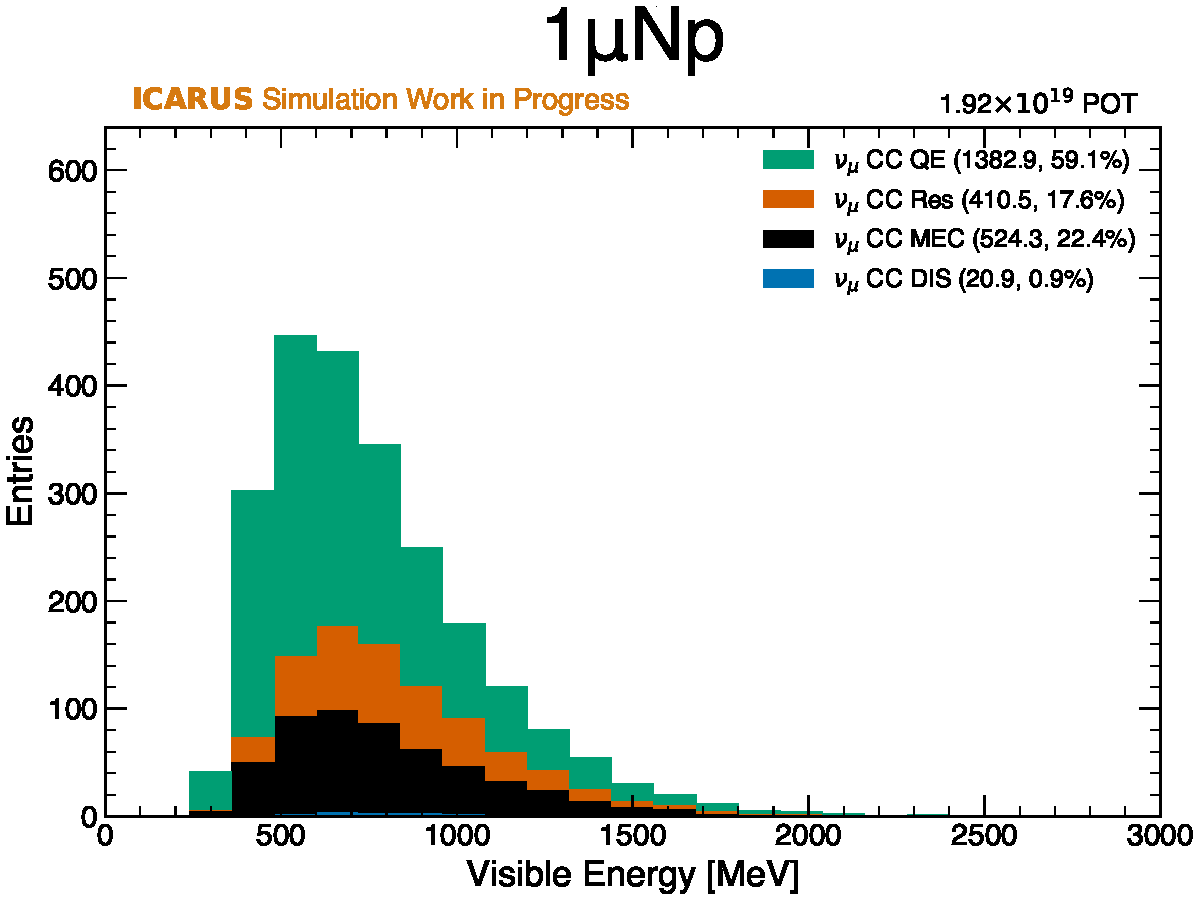
\includegraphics[width=0.48\textwidth]{figures/neutrino_selection/signal_hist1d_1muNp_visible_energy.pdf}\\
    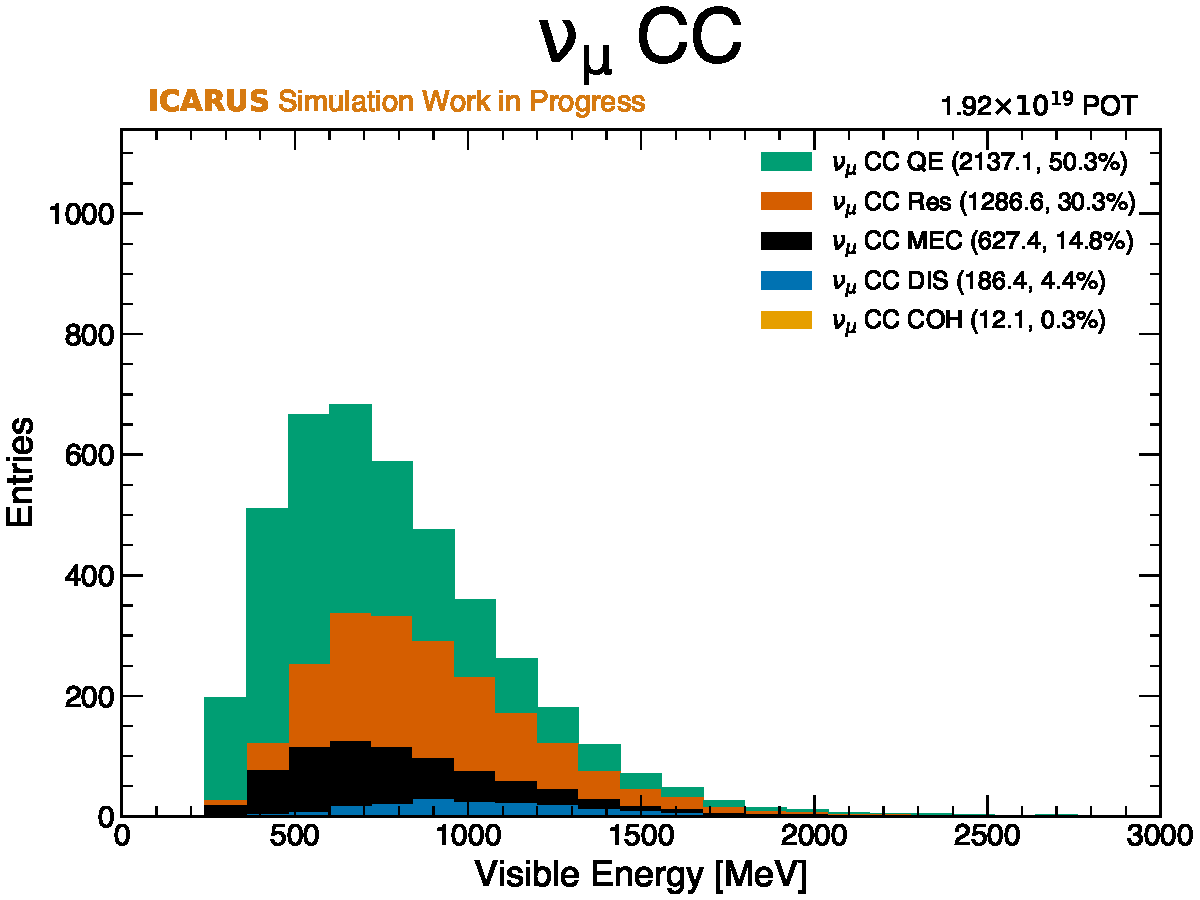
\includegraphics[width=0.48\textwidth]{figures/neutrino_selection/signal_hist1d_1muX_visible_energy.pdf}\\
    \caption{Total visible energy of the interaction for each of the signal channels: from top to bottom $\mathrm{1\mu 1p}$, $\mathrm{1\mu Np}$, and $\nu_\mu$ CC inclusive.}
    \label{fig:visible_energy}
\end{figure}

\paragraph{Muon Transverse Momentum ($\mathbf{p_T^\mu}$):}
The component of muon momentum perpendicular to the neutrino beam direction. This should generally be balanced by the transverse momentum of the hadronic system in the absence of final state interactions, as described in more detail below in the text on kinematic imbalance variables.

\paragraph{Leading Proton Transverse Momentum ($\mathbf{p_T^p}$):}
The component of the momentum of the most energetic primary proton perpendicular to the neutrino beam direction.

\begin{figure}[!htb]
    \centering
    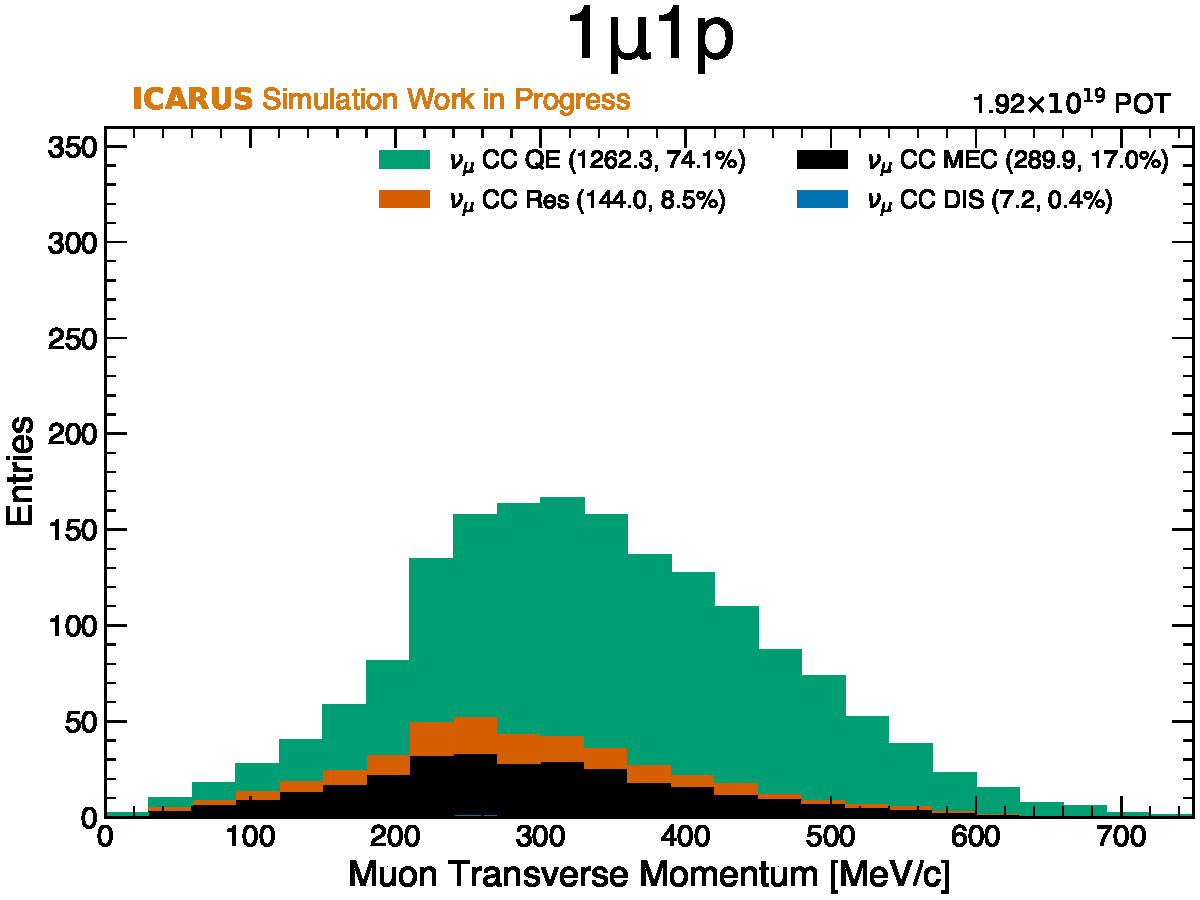
\includegraphics[width=0.48\textwidth]{figures/neutrino_selection/signal_hist1d_1mu1p_muon_pt.pdf}
    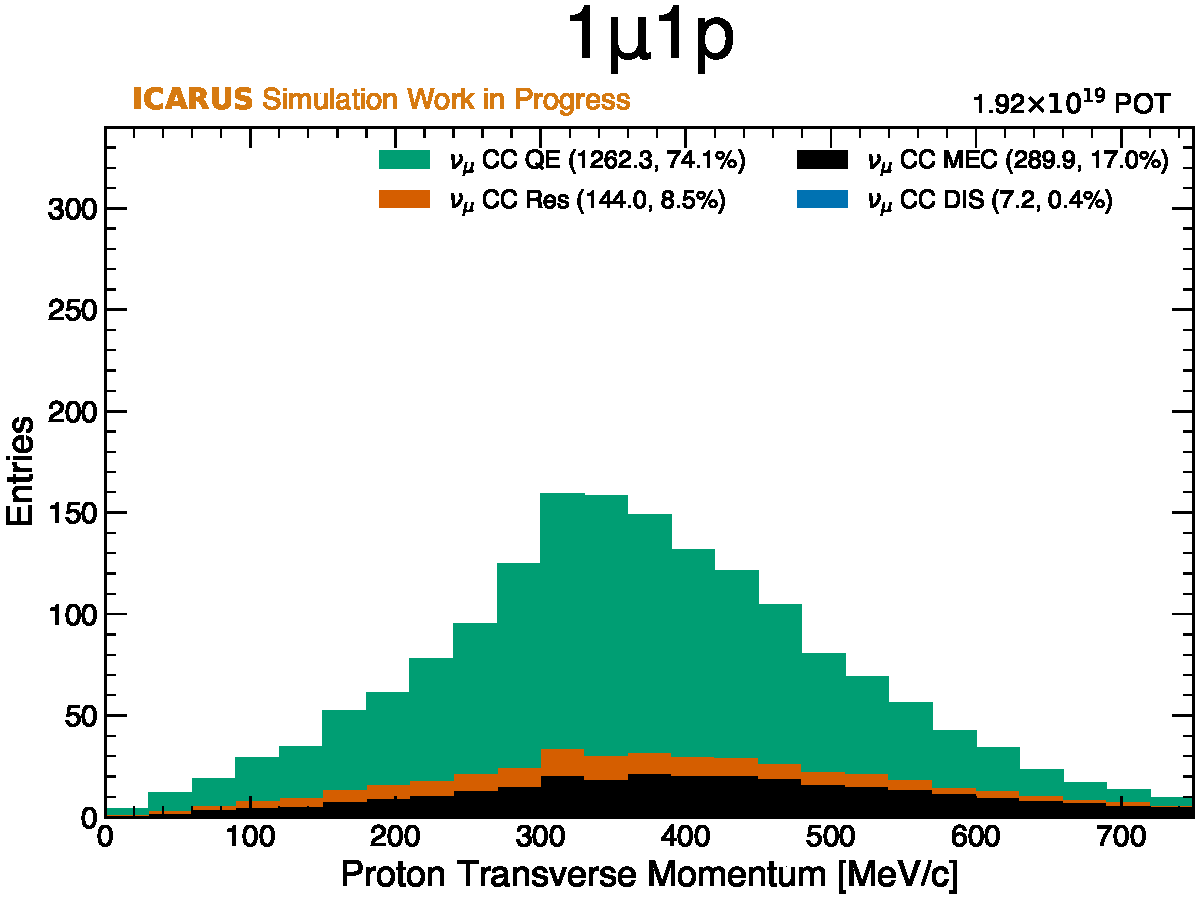
\includegraphics[width=0.48\textwidth]{figures/neutrino_selection/signal_hist1d_1mu1p_proton_pt.pdf}
    \\
    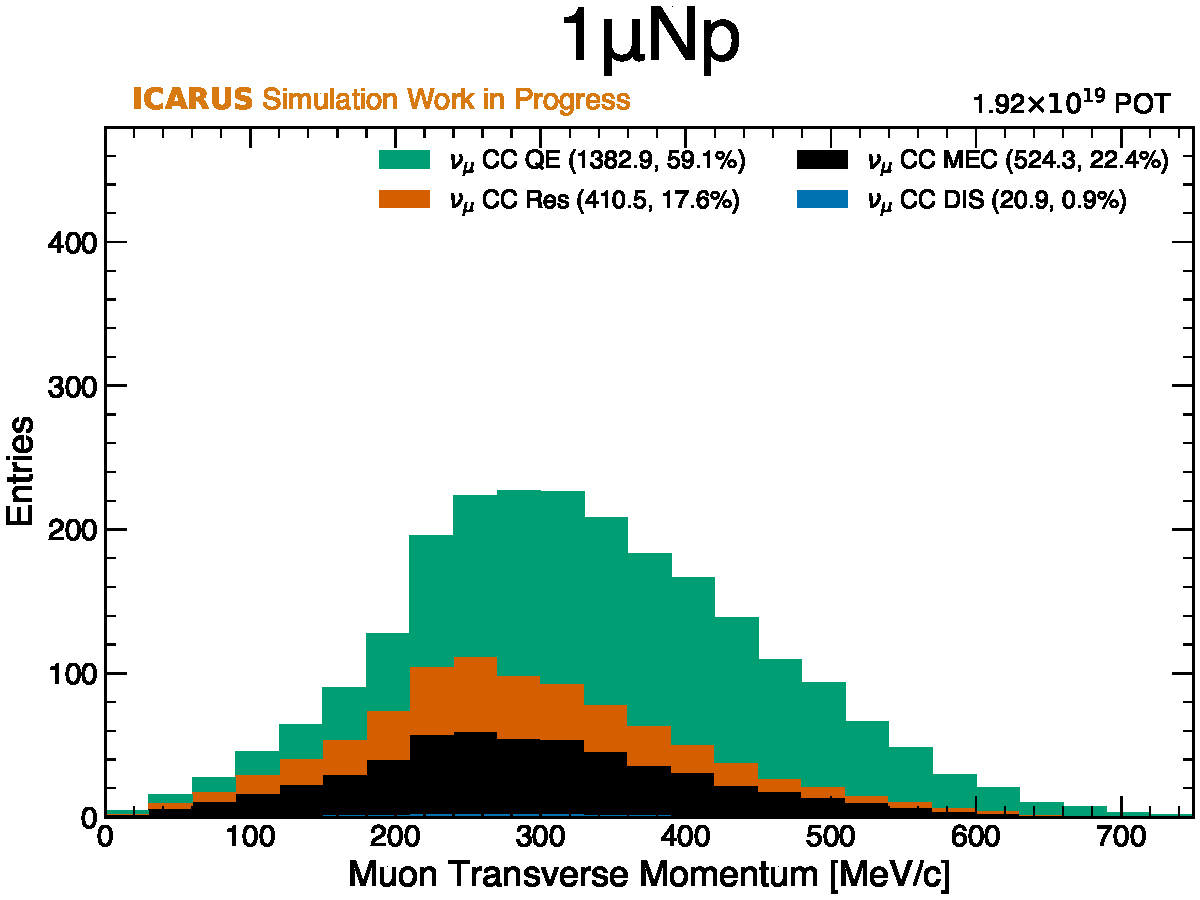
\includegraphics[width=0.48\textwidth]{figures/neutrino_selection/signal_hist1d_1muNp_muon_pt.pdf}
    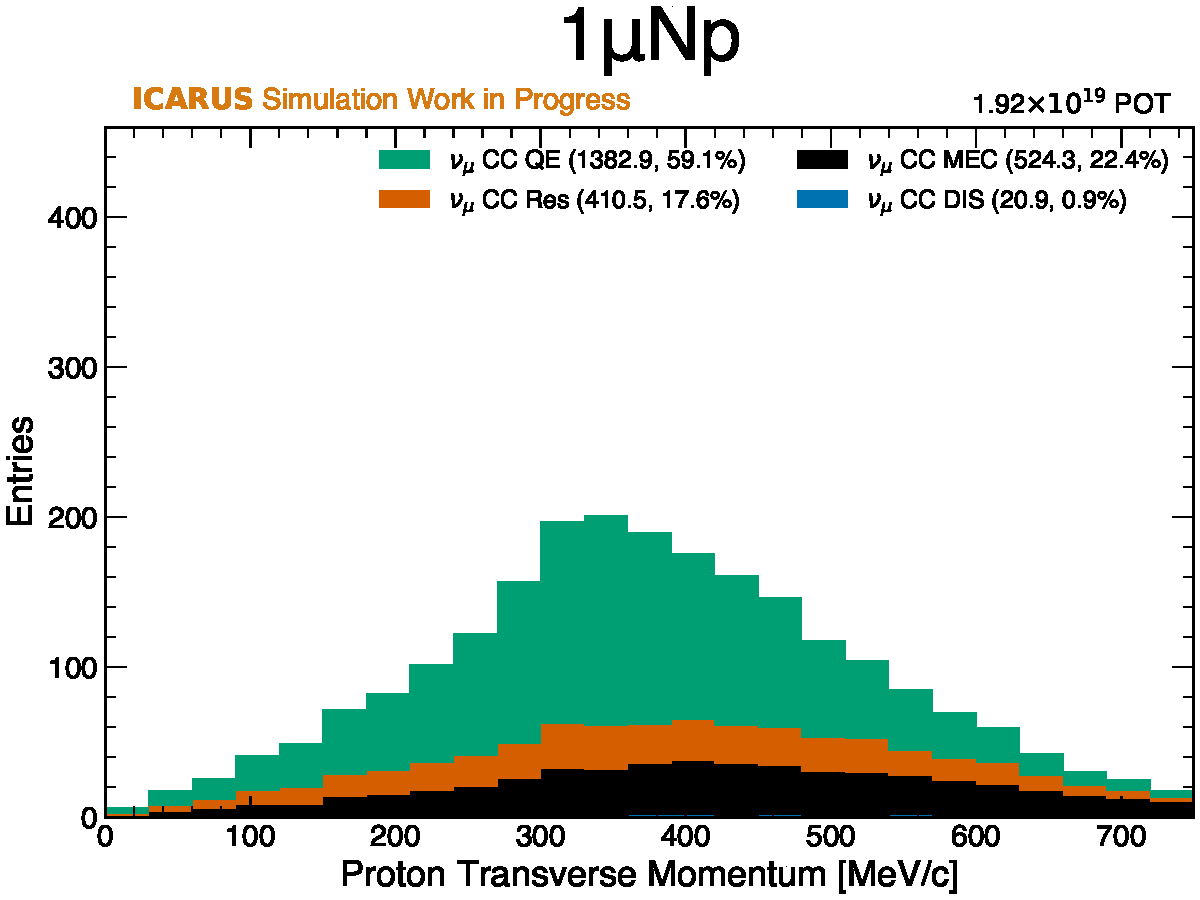
\includegraphics[width=0.48\textwidth]{figures/neutrino_selection/signal_hist1d_1muNp_proton_pt.pdf}
    \\
    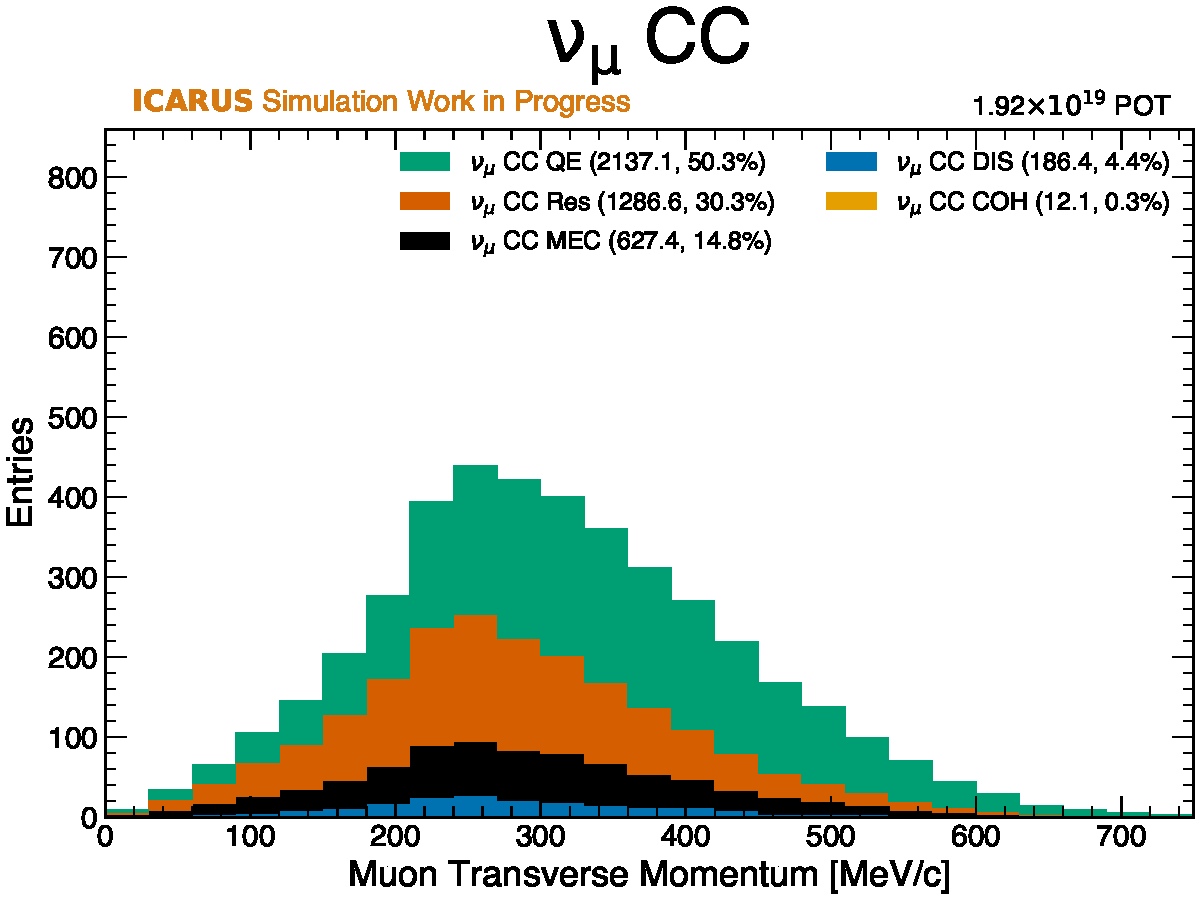
\includegraphics[width=0.48\textwidth]{figures/neutrino_selection/signal_hist1d_1muX_muon_pt.pdf}
    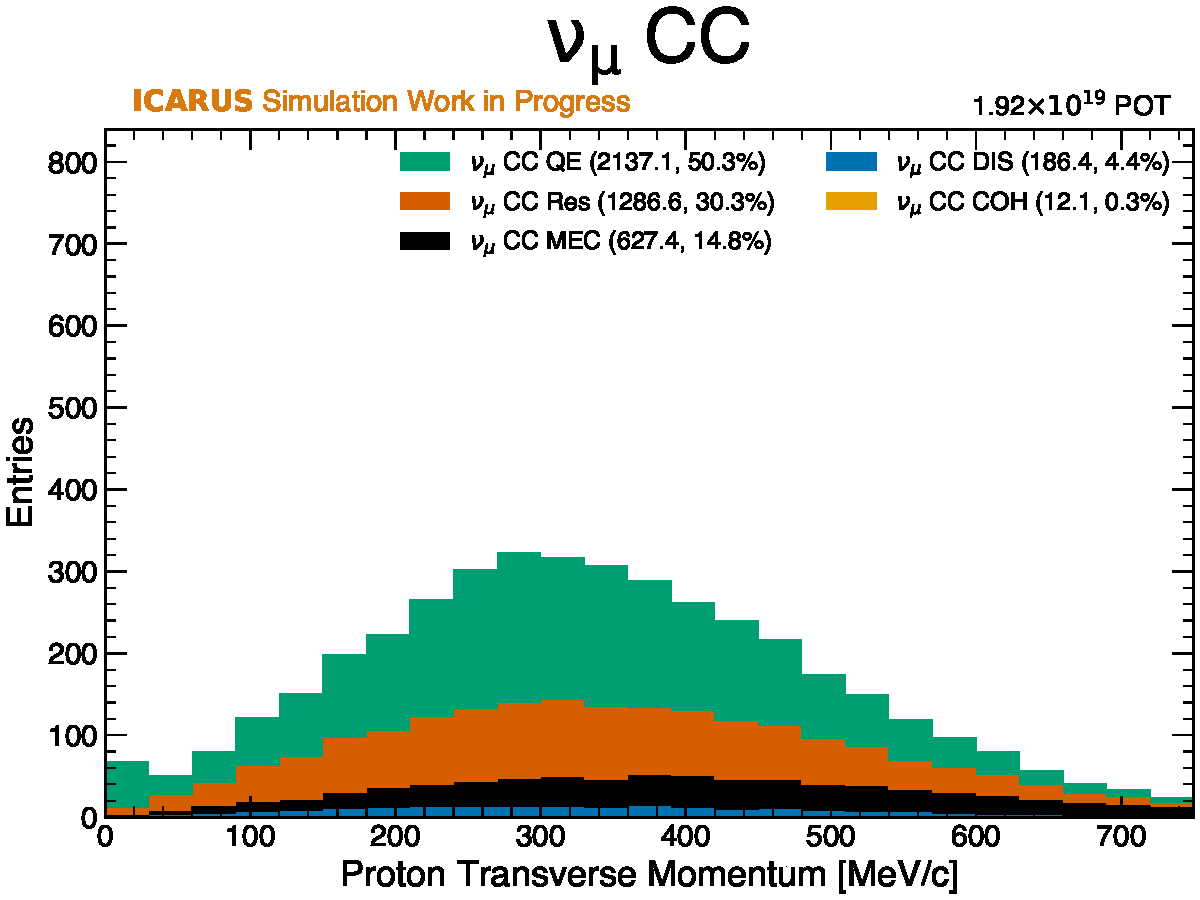
\includegraphics[width=0.48\textwidth]{figures/neutrino_selection/signal_hist1d_1muX_proton_pt.pdf}
    \caption{Transverse momentum of the muon (left) and the most energetic proton (right) for each of the three signal channels: from top to bottom $\mathrm{1\mu 1p}$, $\mathrm{1\mu Np}$, and $\nu_\mu$ CC inclusive.}
    \label{fig:muon_proton_pt}
\end{figure}

\paragraph{Muon Polar Angle ($\mathbf{\theta_\mu}$):}
The polar angle of the muon calculated with respect to the neutrino beam direction (z-axis):
\begin{equation}
    \theta_\mu = \arccos\left(\frac{p^\mu_z}{p^\mu}\right)
\end{equation}

\paragraph{Muon Azimuthal Angle ($\mathbf{\phi_\mu}$):}
The azimuthal angle of the muon calculated with respect to the neutrino beam direction (z-axis):
\begin{equation}
    \phi_\mu = \arccos\left(\frac{p^\mu_x}{p^\mu_T}\right)
\end{equation}

\begin{figure}[!htb]
    \centering
    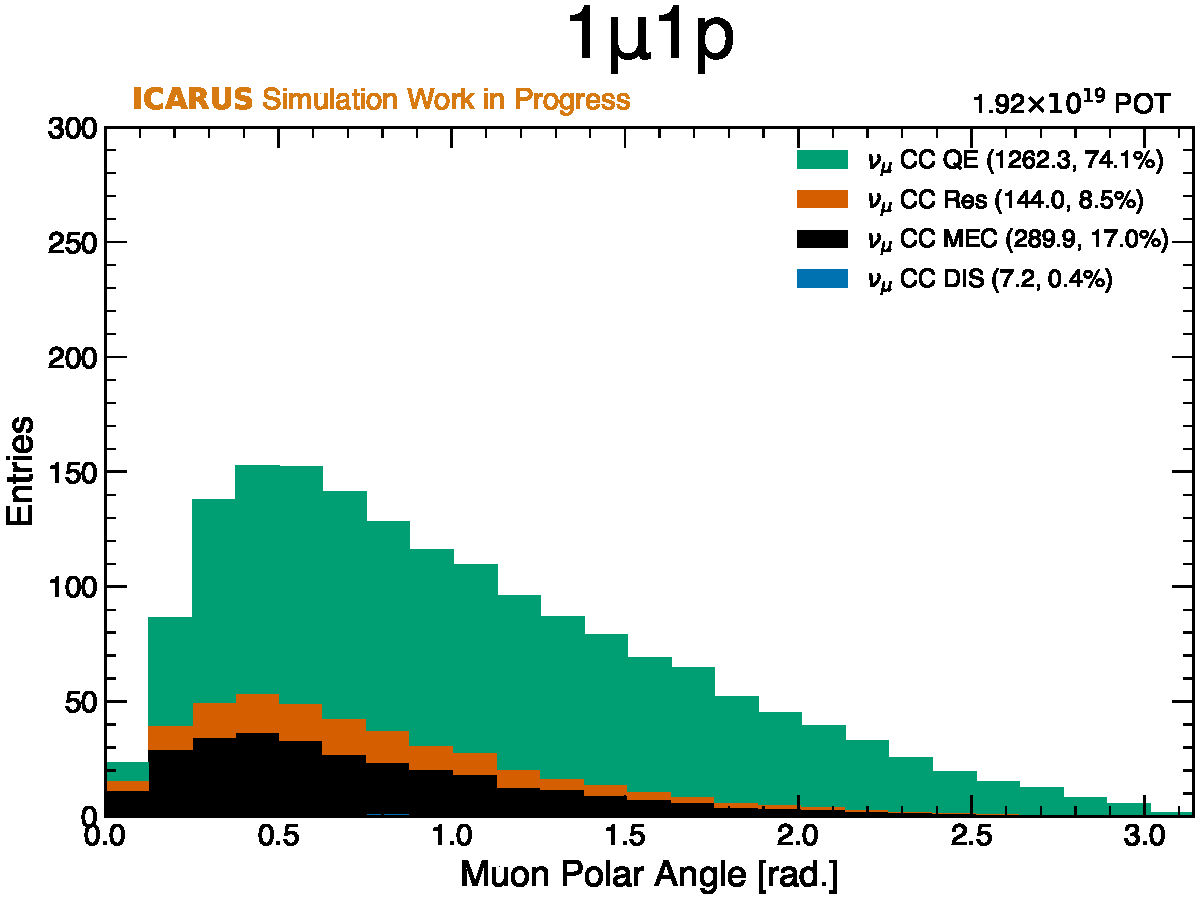
\includegraphics[width=0.48\textwidth]{figures/neutrino_selection/signal_hist1d_1mu1p_muon_polar_angle.pdf}
    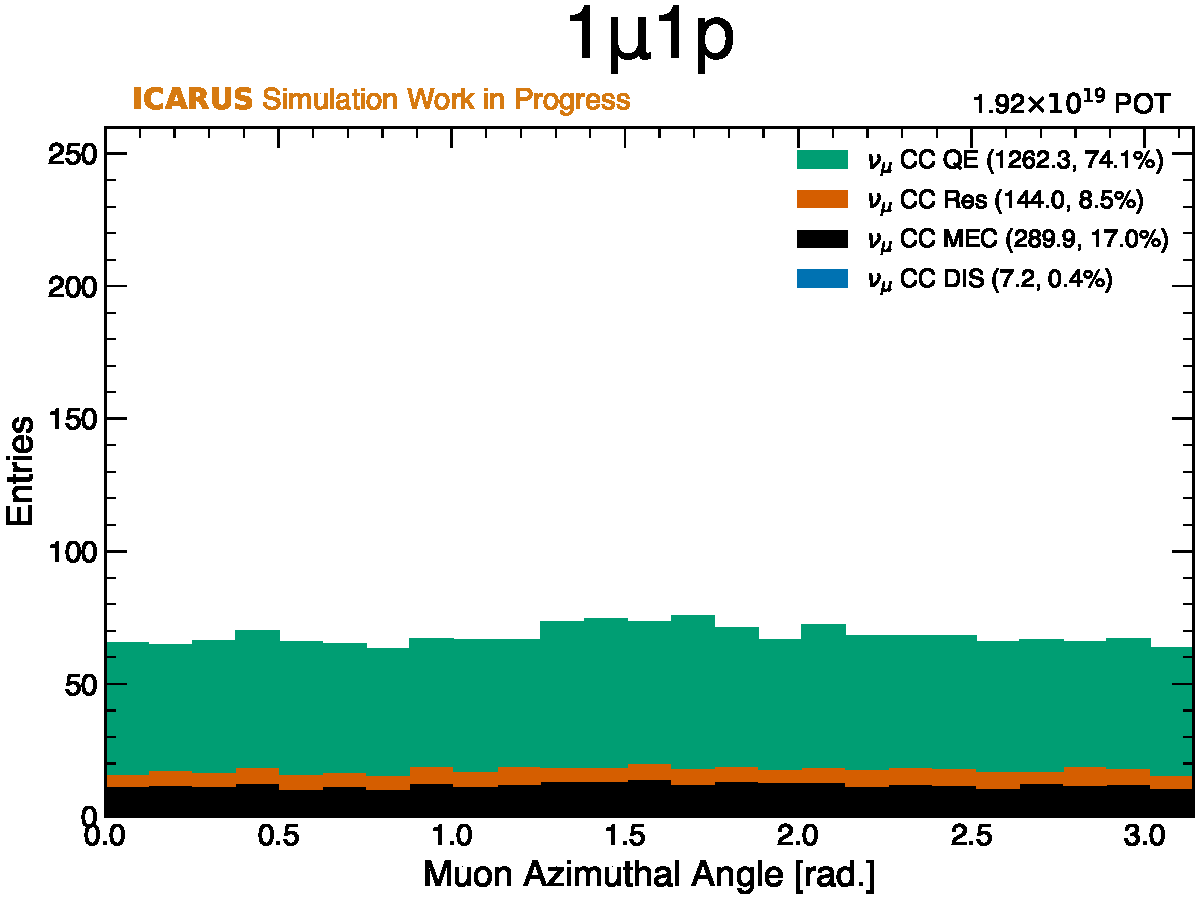
\includegraphics[width=0.48\textwidth]{figures/neutrino_selection/signal_hist1d_1mu1p_muon_azimuthal_angle.pdf}
    \\
    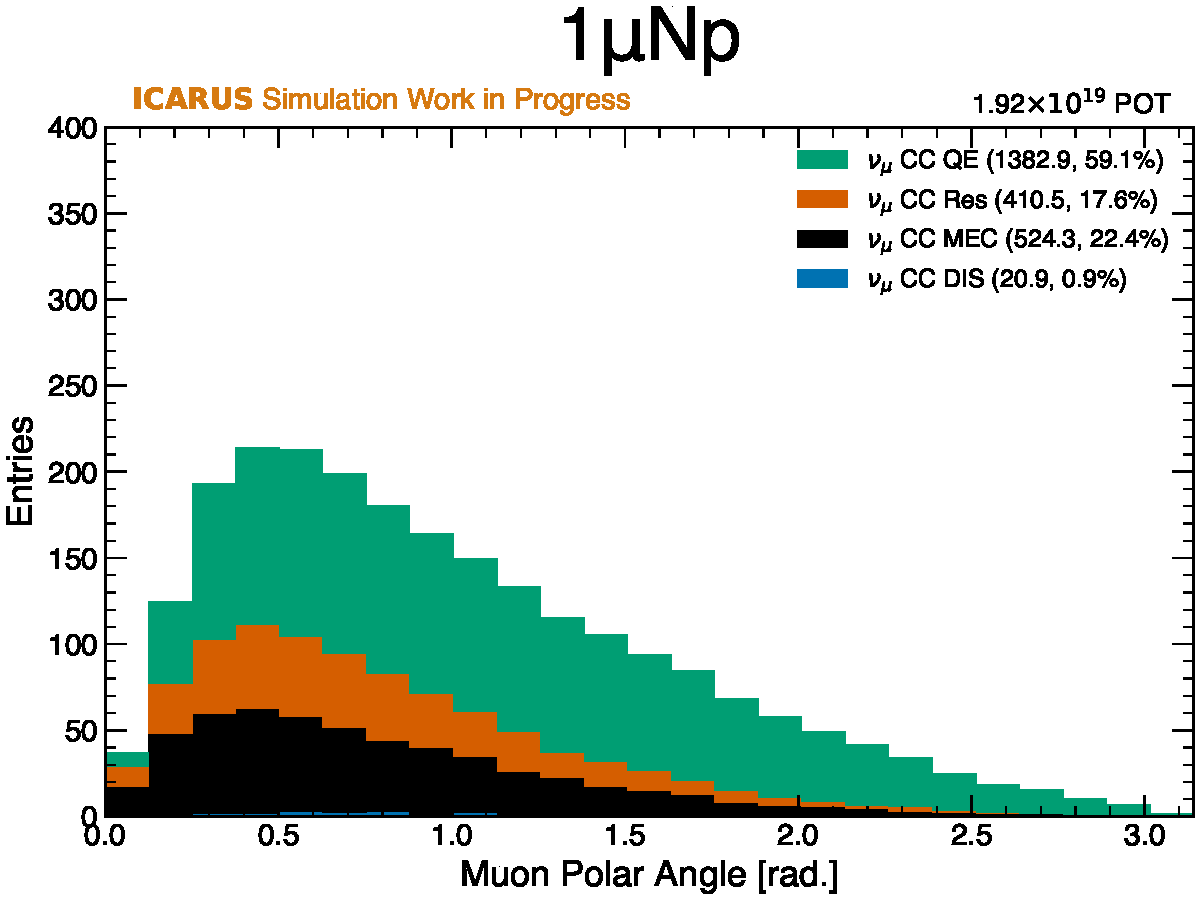
\includegraphics[width=0.48\textwidth]{figures/neutrino_selection/signal_hist1d_1muNp_muon_polar_angle.pdf}
    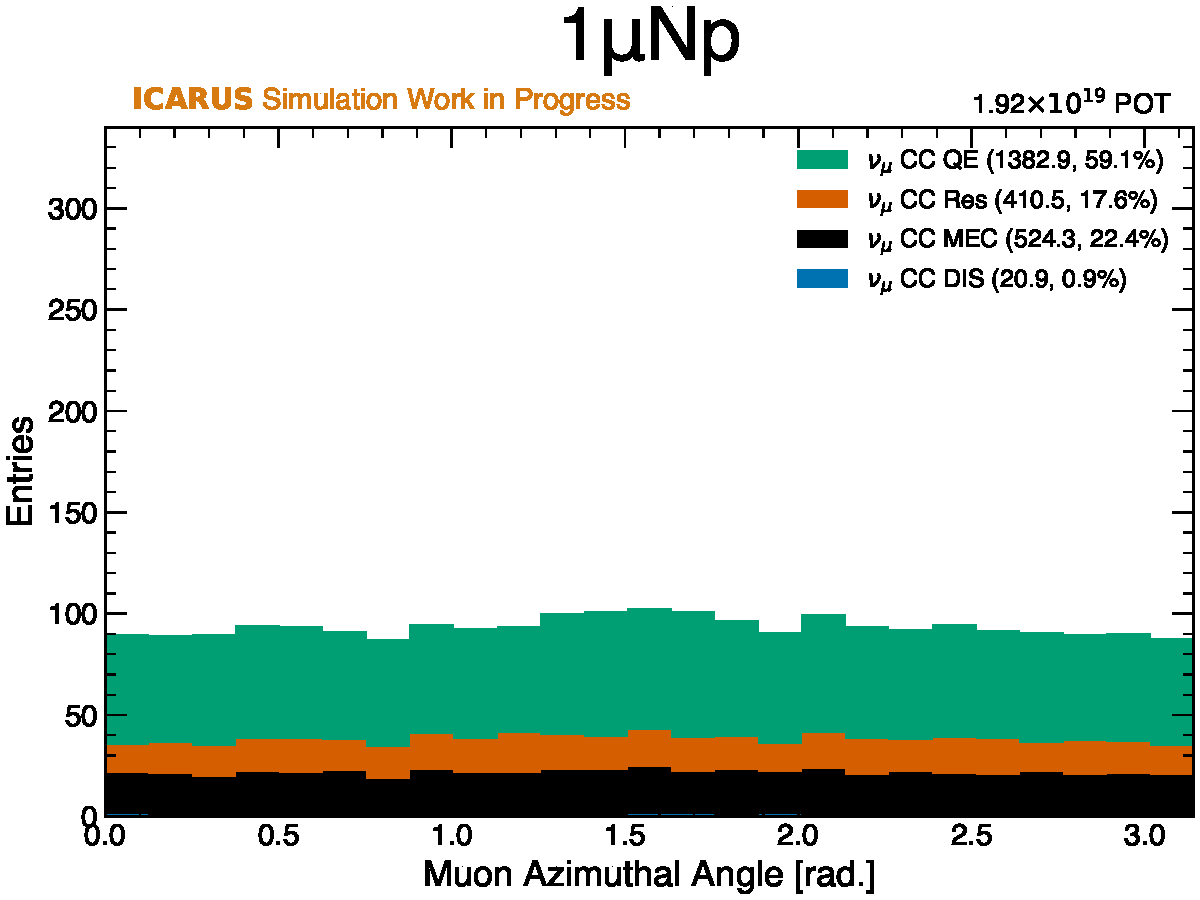
\includegraphics[width=0.48\textwidth]{figures/neutrino_selection/signal_hist1d_1muNp_muon_azimuthal_angle.pdf}
    \\
    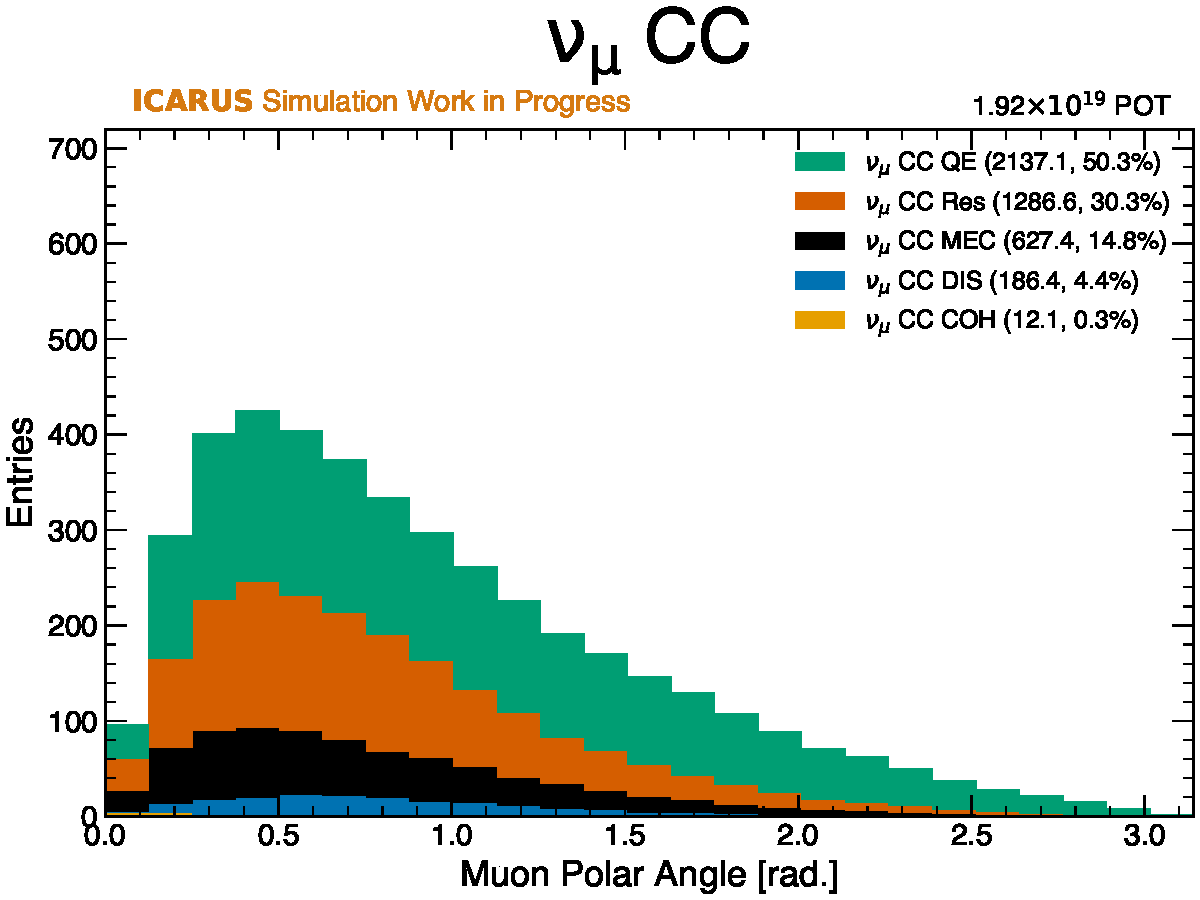
\includegraphics[width=0.48\textwidth]{figures/neutrino_selection/signal_hist1d_1muX_muon_polar_angle.pdf}
    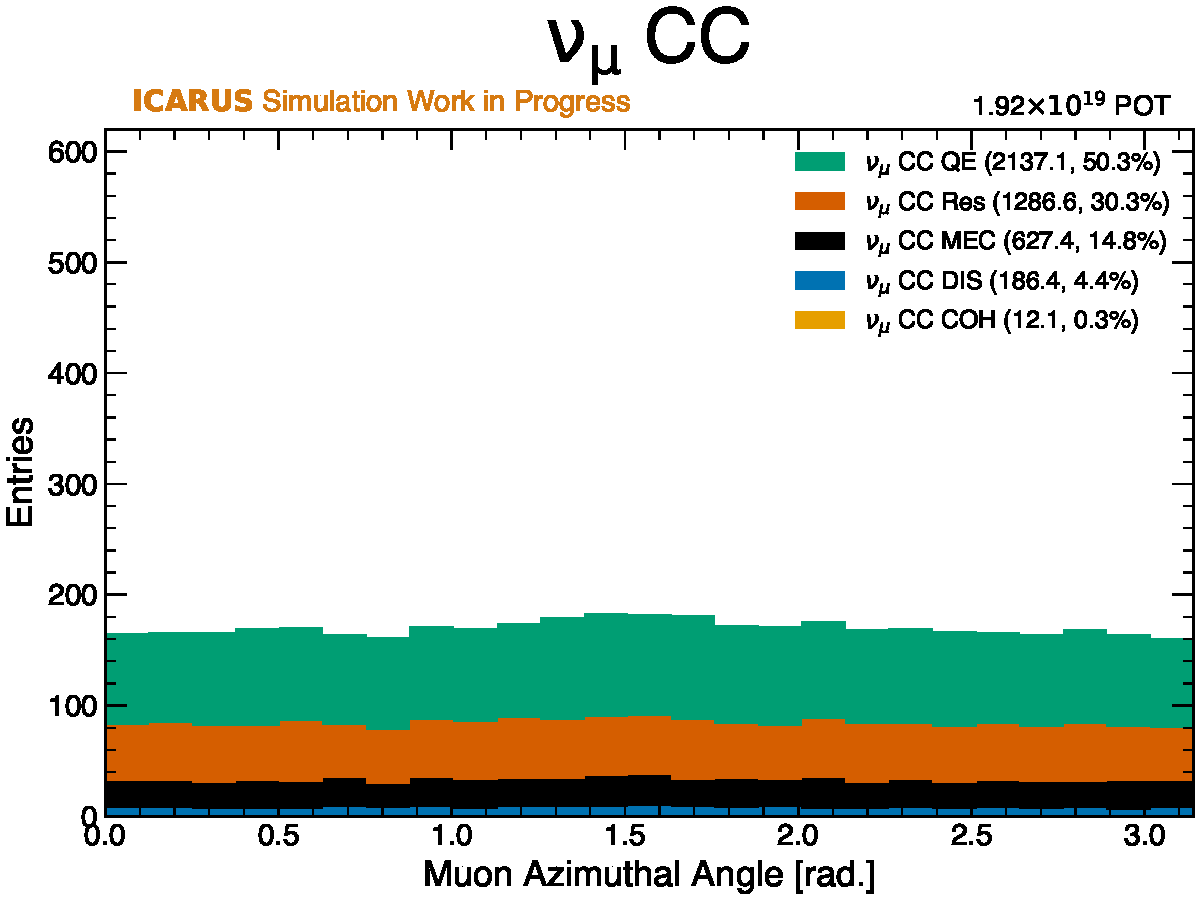
\includegraphics[width=0.48\textwidth]{figures/neutrino_selection/signal_hist1d_1muX_muon_azimuthal_angle.pdf}
    \caption{Polar angle (left) and azimuthal angle (right) of the muon for each of the three signal channels: from top to bottom $\mathrm{1\mu 1p}$, $\mathrm{1\mu Np}$, and $\nu_\mu$ CC inclusive.}
    \label{fig:muon_angles}
\end{figure}

\paragraph{Opening Angle ($\mathbf{\theta_{\mu p}}$):}
The angle between the muon and the leading proton.
\begin{equation}
    \theta_{\mu p} = \arccos\left(\frac{\vec{p\ }^\mu \cdot \vec{p\ }^p}{|\vec{p\ }^\mu||\vec{p\ }^p|}\right)
\end{equation}

\begin{figure}[!htb]
    \centering
    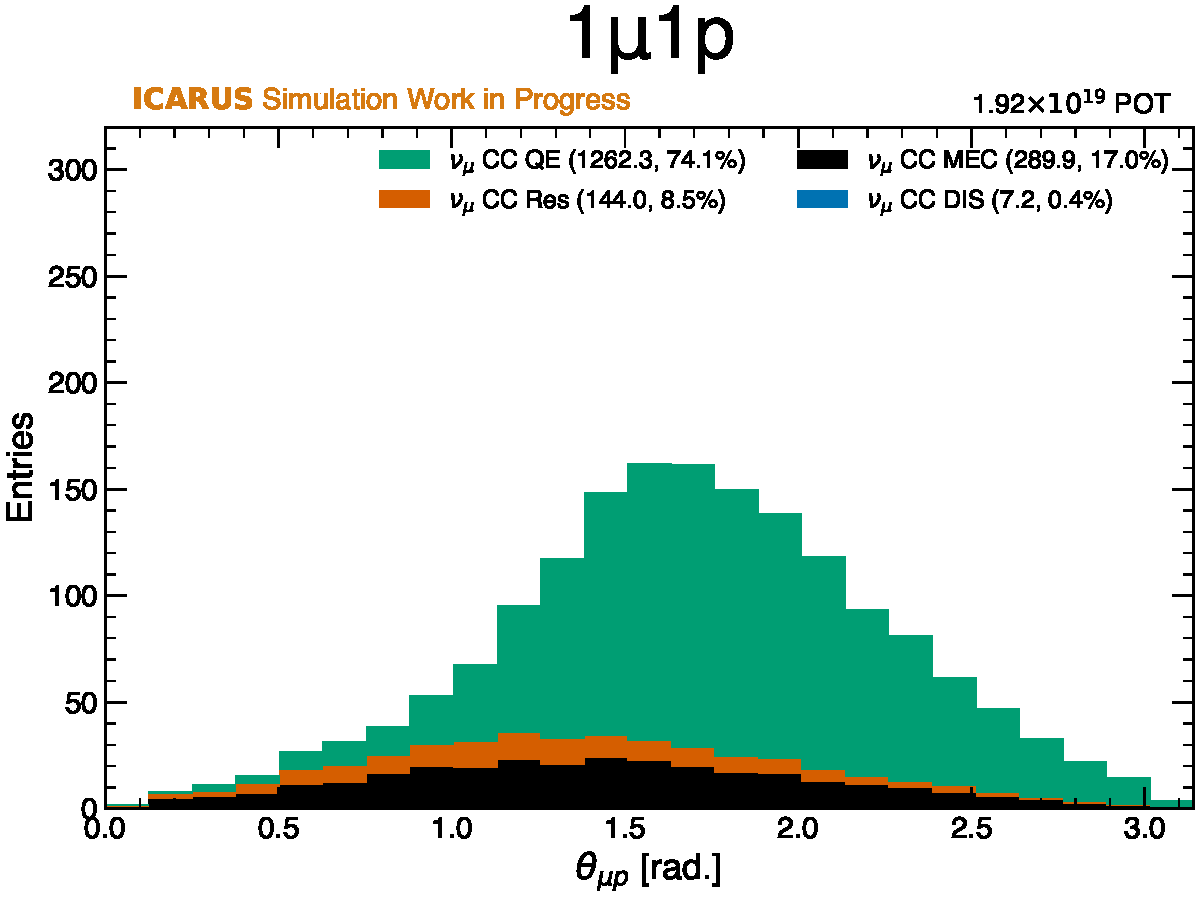
\includegraphics[width=0.48\textwidth]{figures/neutrino_selection/signal_hist1d_1mu1p_opening_angle.pdf}\\
    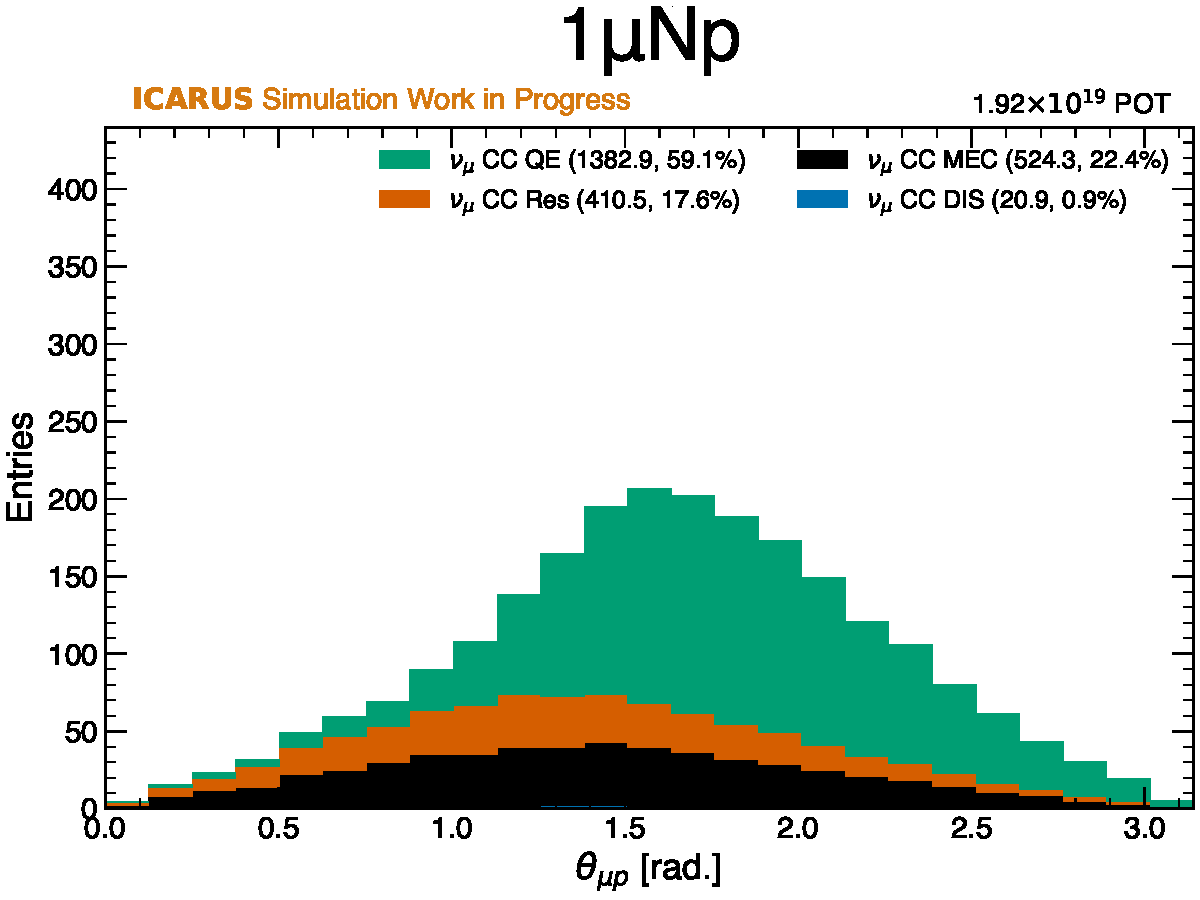
\includegraphics[width=0.48\textwidth]{figures/neutrino_selection/signal_hist1d_1muNp_opening_angle.pdf}\\
    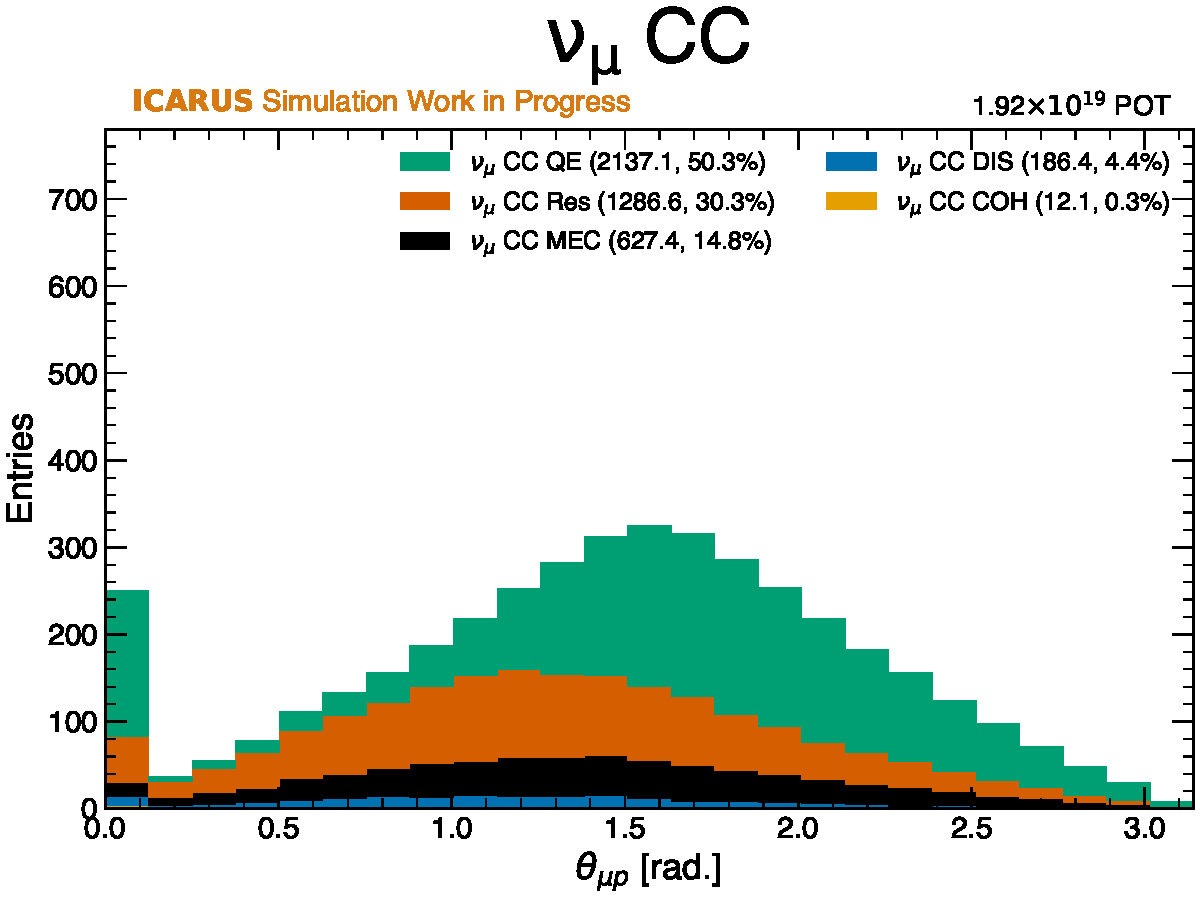
\includegraphics[width=0.48\textwidth]{figures/neutrino_selection/signal_hist1d_1muX_opening_angle.pdf}\\
    \caption{The muon-proton opening angle for each of the three signal channels: from top to bottom $\mathrm{1\mu 1p}$, $\mathrm{1\mu Np}$, and $\nu_\mu$ CC inclusive. The peak at the lowest bin in the inclusive channel is from interactions where no proton is present.}
    \label{fig:opening_angle}
\end{figure}

\subsubsection{Kinematic Imbalance Variables}
\label{sec:kinematic_imbalance_variables}

The axis of the beam defines the direction along which the momentum of the interacting neutrino is oriented. The transverse plane is defined as the plane perpendicular to the neutrino beam direction, while the longitudinal direction is defined as oriented along the neutrino beam direction. From conservation of momentum, the momentum in the transverse plane should sum to zero in the absence of initial state nucleon transverse momentum and final state interactions (FSI). Fermi motion inside the nucleus produces non-zero transverse momentum even for quasi-elastic (QE) interactions. More complex interactions such as resonant pion production and deep inelastic scattering can produce final states similar to QE interactions, but with additional transverse momentum that populates the region above the Fermi momentum. These variables are natural choices for probing the effects of FSI and for measuring neutrino interaction cross sections.

In the ICARUS geometry, the beam axis is defined as the $z$-axis, and the transverse plane is correspondingly the $x$-$y$ plane. For the signal definitions considered in this analysis, there exists a single muon and a combined hadronic system, respectively having momentum $\vec{p\ }^\mu$ and $\vec{p\ }^h$ and transverse components $\vec{p\ }^\mu_T$ and $\vec{p\ }^h_T$. The transverse component of the momentum transfer to the nucleus, $\vec{q}_T$, is defined as equal and opposite to $\vec{p\ }^\mu_T$. Schematically, this is shown in Figure \ref{fig:kinematic_imbalance} within the transverse plane. This formalism, presented in detail in \cite{MicroBooNE2024}, leads to the introduction of several variables:

\begin{figure}
    \centering
    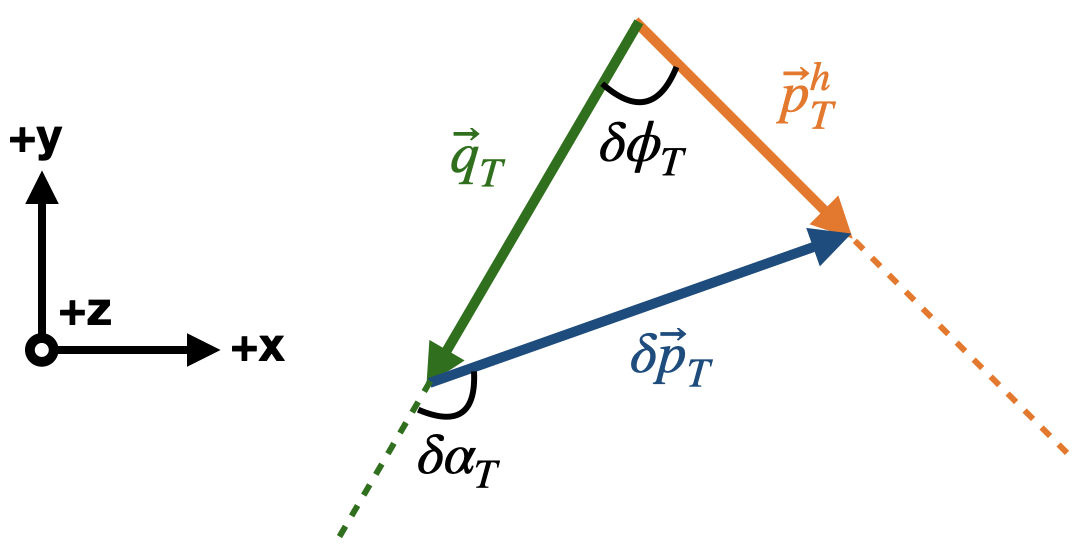
\includegraphics[width=0.5\textwidth]{figures/neutrino_selection/kinematic_imbalance_diagram.png}
    \caption{Diagram showing the each of the chosen kinematic imbalance variables in the transverse plane.}
    \label{fig:kinematic_imbalance}
\end{figure}

\paragraph{$\mathbf{\delta p_T}$:}
The magnitude of the vector difference between the transverse momentum of the muon and the hadronic system. This variable quantifies the amount of transverse momentum that is not accounted for by the reconstructed particles. Large values of this quantity exceeding the Fermi momentum are indicative of FSI.
\begin{equation}
    \delta p_T = \left|\vec{p\ }^\mu_T - \vec{p\ }^h_T\right|
\end{equation}

\begin{figure}[!htb]
    \centering
    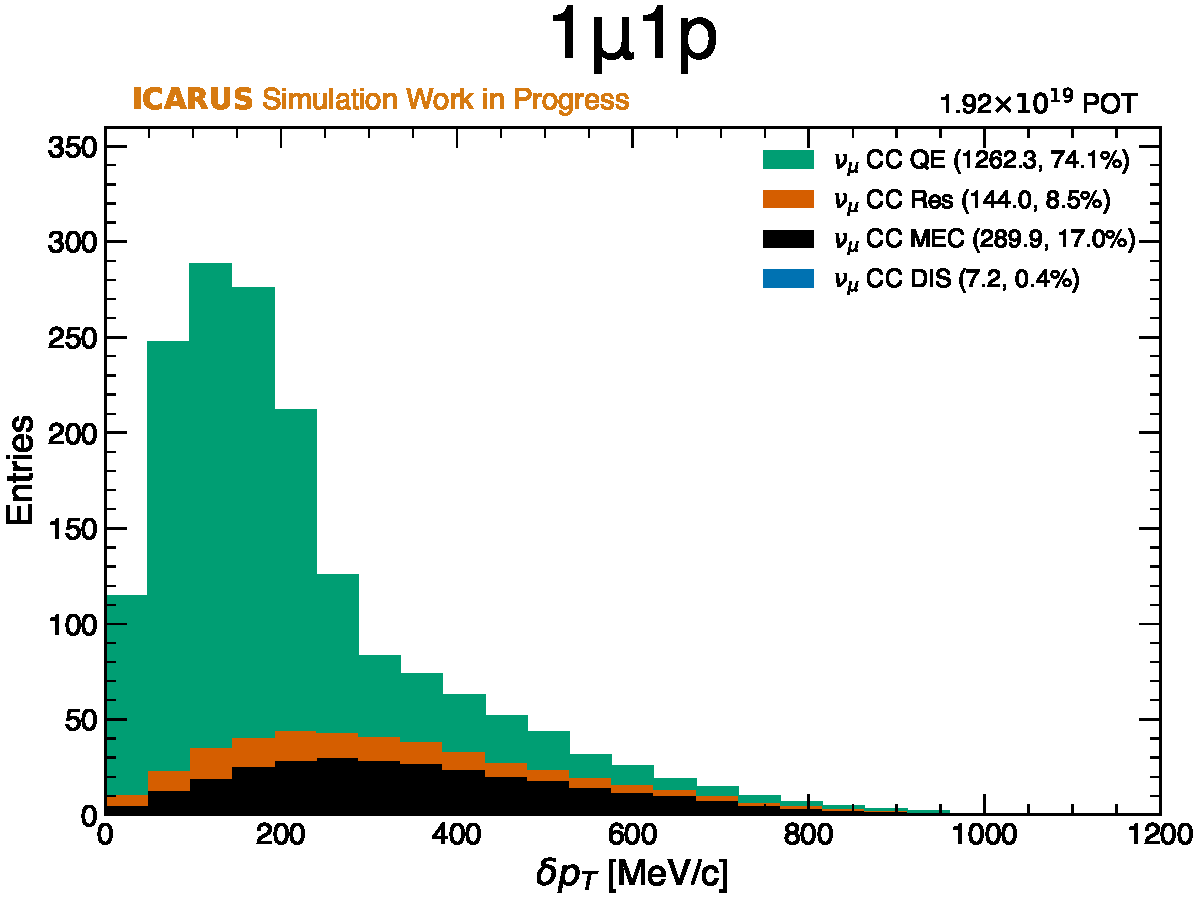
\includegraphics[width=0.48\textwidth]{figures/neutrino_selection/signal_hist1d_1mu1p_delta_pT.pdf}\\
    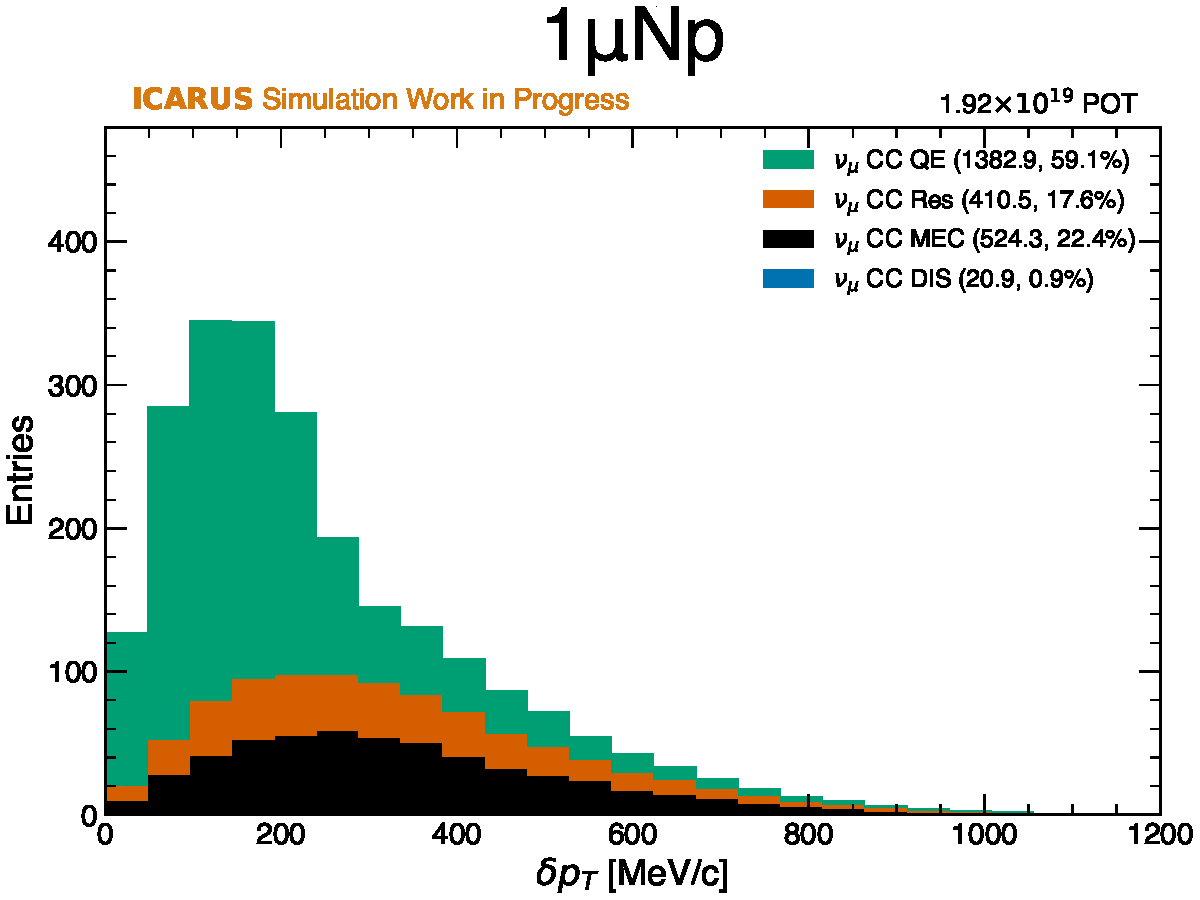
\includegraphics[width=0.48\textwidth]{figures/neutrino_selection/signal_hist1d_1muNp_delta_pT.pdf}\\
    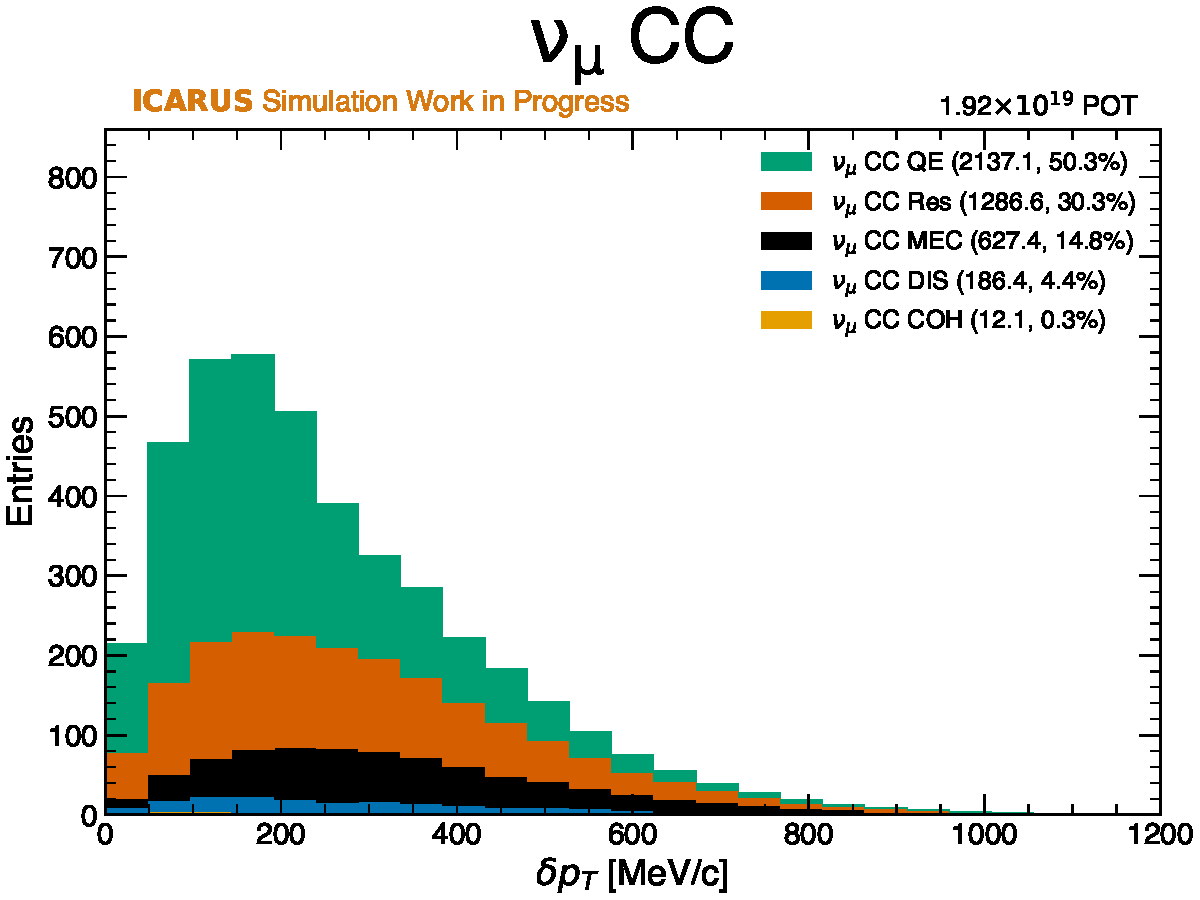
\includegraphics[width=0.48\textwidth]{figures/neutrino_selection/signal_hist1d_1muX_delta_pT.pdf}\\
    \caption{Transverse momentum of the interaction for each of the three signal channels: from top to bottom $\mathrm{1\mu 1p}$, $\mathrm{1\mu Np}$, and $\nu_\mu$ CC inclusive.}
    \label{fig:delta_pT}
\end{figure}

\paragraph{$\mathbf{\delta \phi_T}$:}
The angle between the the transverse momentum transfer vector and the transverse momentum of the hadronic system. In the case of a free and stationary nucleon target, this angle would be zero. Initial state motion leads to small values of this quantity, while FSI can lead to larger values.
\begin{equation}
    \delta \phi_T = \arccos\left(\frac{\vec{p\ }^h_T \cdot \vec{q}_T}{|\vec{p\ }^h_T||\vec{q}_T|}\right)
\end{equation}

\paragraph{$\mathbf{\delta \alpha_T}$:}
The angle between the transverse momentum transfer vector and transverse missing momentum vector. This angle is less sensitive to the initial state motion of the nucleons, but is sensitive to FSI. In the absence of FSI, this quantity does not have a preferred orientation.
\begin{equation}
    \delta \alpha_T = \arccos\left(\frac{\vec{q}_T \cdot \delta \vec{p\ }_T}{|\vec{q}_T||\delta \vec{p\ }_T|}\right)
\end{equation}

\begin{figure}[!htb]
    \centering
    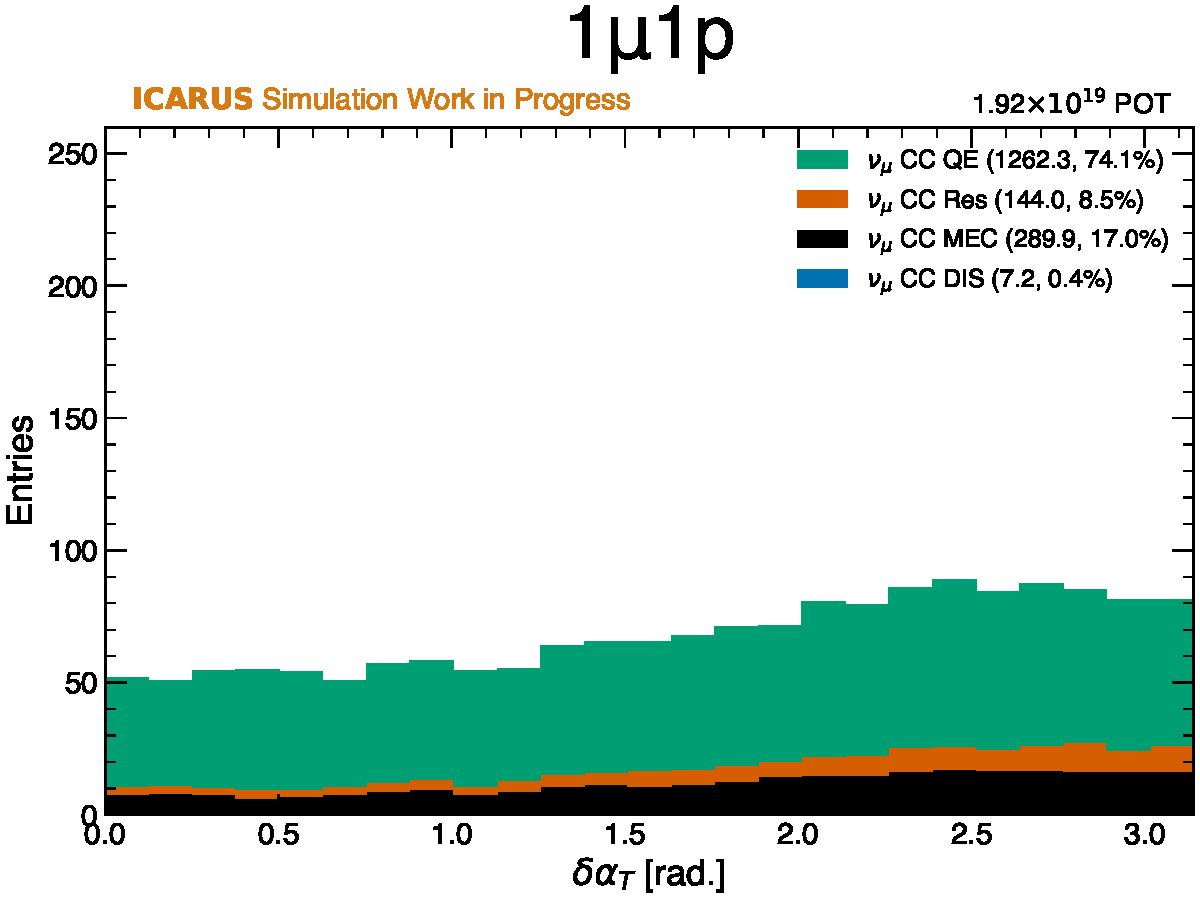
\includegraphics[width=0.48\textwidth]{figures/neutrino_selection/signal_hist1d_1mu1p_delta_alphaT.pdf}
    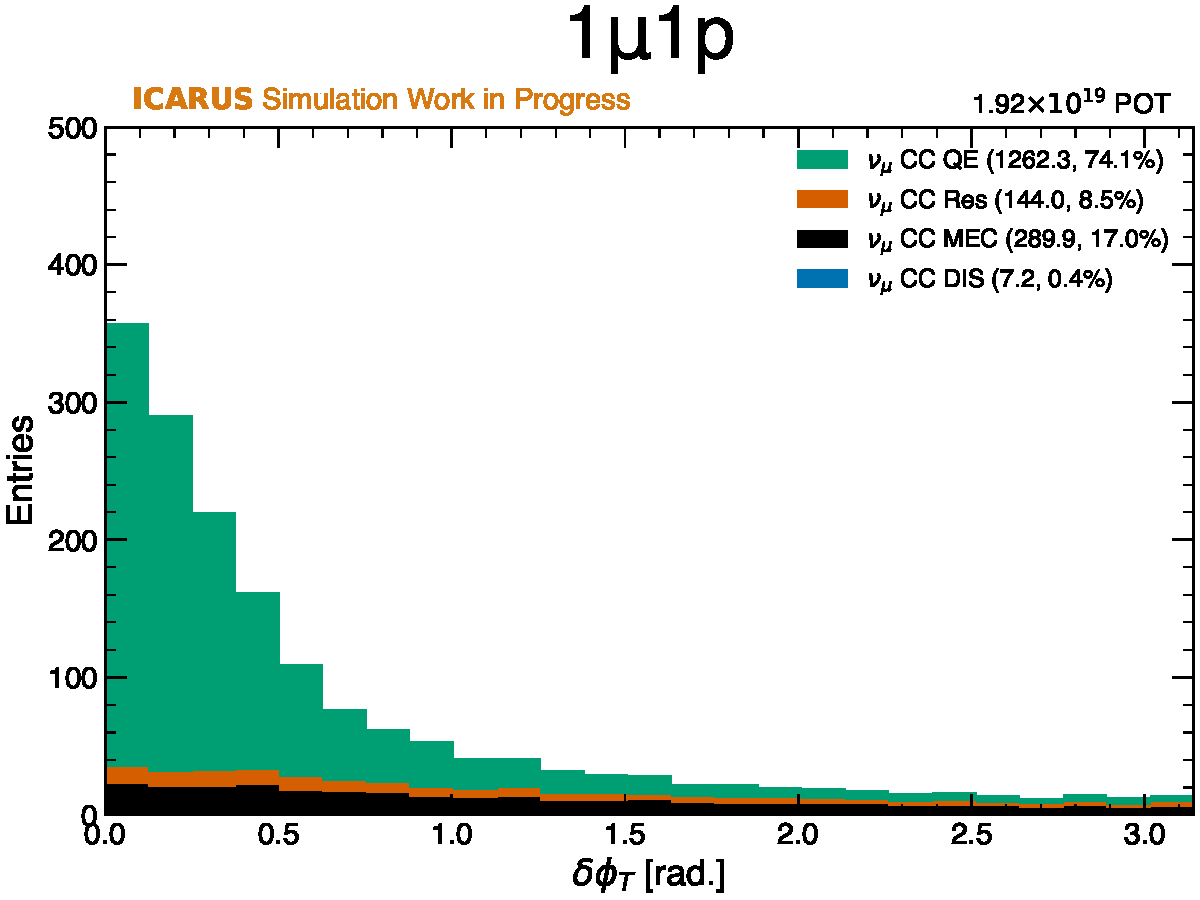
\includegraphics[width=0.48\textwidth]{figures/neutrino_selection/signal_hist1d_1mu1p_delta_phiT.pdf}
    \\
    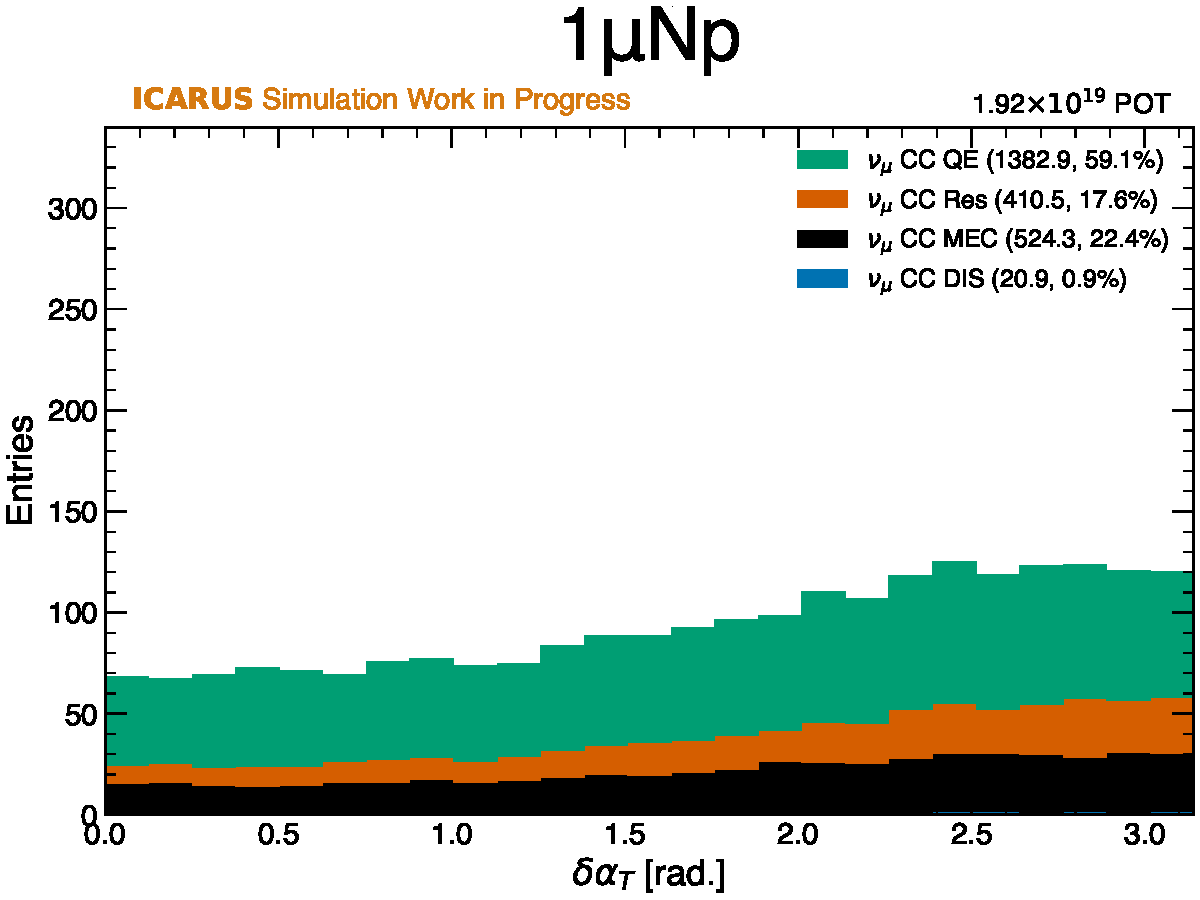
\includegraphics[width=0.48\textwidth]{figures/neutrino_selection/signal_hist1d_1muNp_delta_alphaT.pdf}
    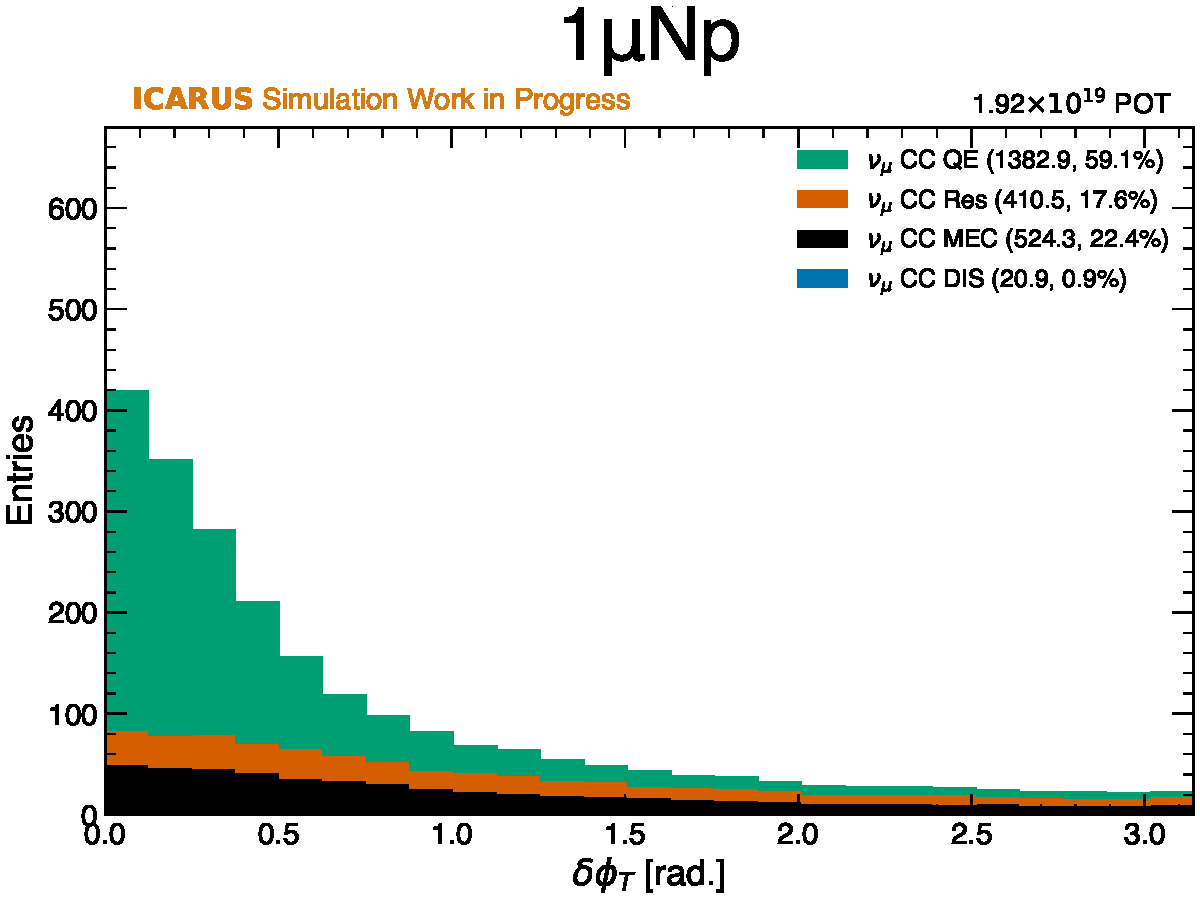
\includegraphics[width=0.48\textwidth]{figures/neutrino_selection/signal_hist1d_1muNp_delta_phiT.pdf}
    \\
    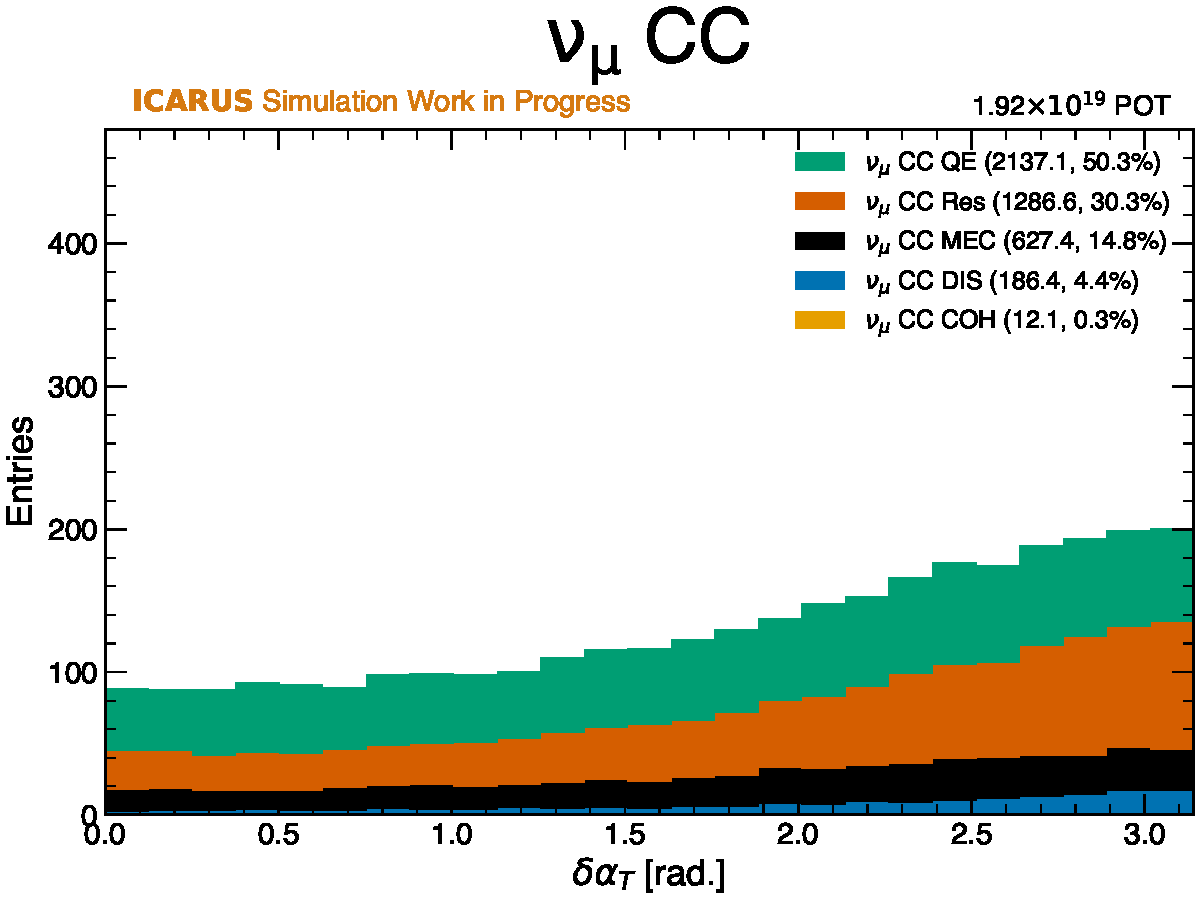
\includegraphics[width=0.48\textwidth]{figures/neutrino_selection/signal_hist1d_1muX_delta_alphaT.pdf}
    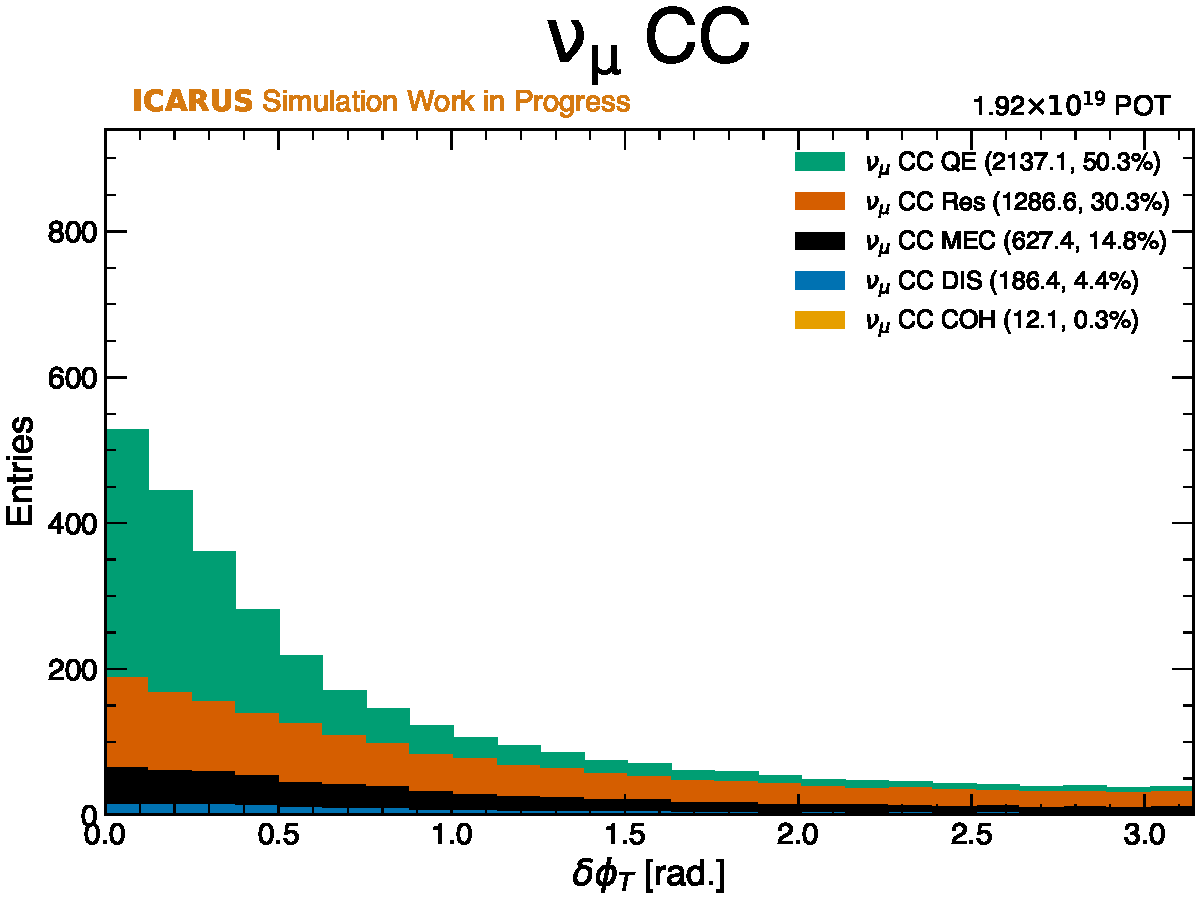
\includegraphics[width=0.48\textwidth]{figures/neutrino_selection/signal_hist1d_1muX_delta_phiT.pdf}
    \caption{Kinematic imbalance variables $\delta \alpha_T$ (left) and $\delta \phi_T$ (right) for each of the three signal channels: from top to bottom $\mathrm{1\mu 1p}$, $\mathrm{1\mu Np}$, and $\nu_\mu$ CC inclusive.}
    \label{fig:kinematic_imbalance_angles}
\end{figure}

\subsubsection{PID Variables}
\label{sec:pid_variables}

Each particle is assigned scores by a GNN, as described in Section \ref{sec:ml_full_chain}, that provide an indication of how likely the particle is to be a muon, proton, or pion for tracks, or an electron or photon for showers. The PID scores are used to assign a particle type to each reconstructed particle. A difference in the distribution of these scores between data and simulation may indicate a bias in the simulation with respect to data, so it is important to validate that these distributions are in agreement with data.

\paragraph{Muon ``Softmax'' PID Score:}
The muon score assigned to the primary muon of the interaction by the reconstruction. A high score near 1 indicates that the particle is likely to be a muon, while a low score near 0 indicates that the particle is not likely to be a muon.

\paragraph{Proton ``Softmax'' PID Score:}
The proton score assigned to the leading proton of the interaction by the reconstruction. A high score near 1 indicates that the particle is likely to be a proton, while a low score near 0 indicates that the particle is not likely to be a proton. This variable is significantly more peaked than the muon score, presumably because the muon and pion are more similar in terms of their energy deposition and track length, so the range of the plot has been restricted.

\begin{figure}[!htb]
    \centering
    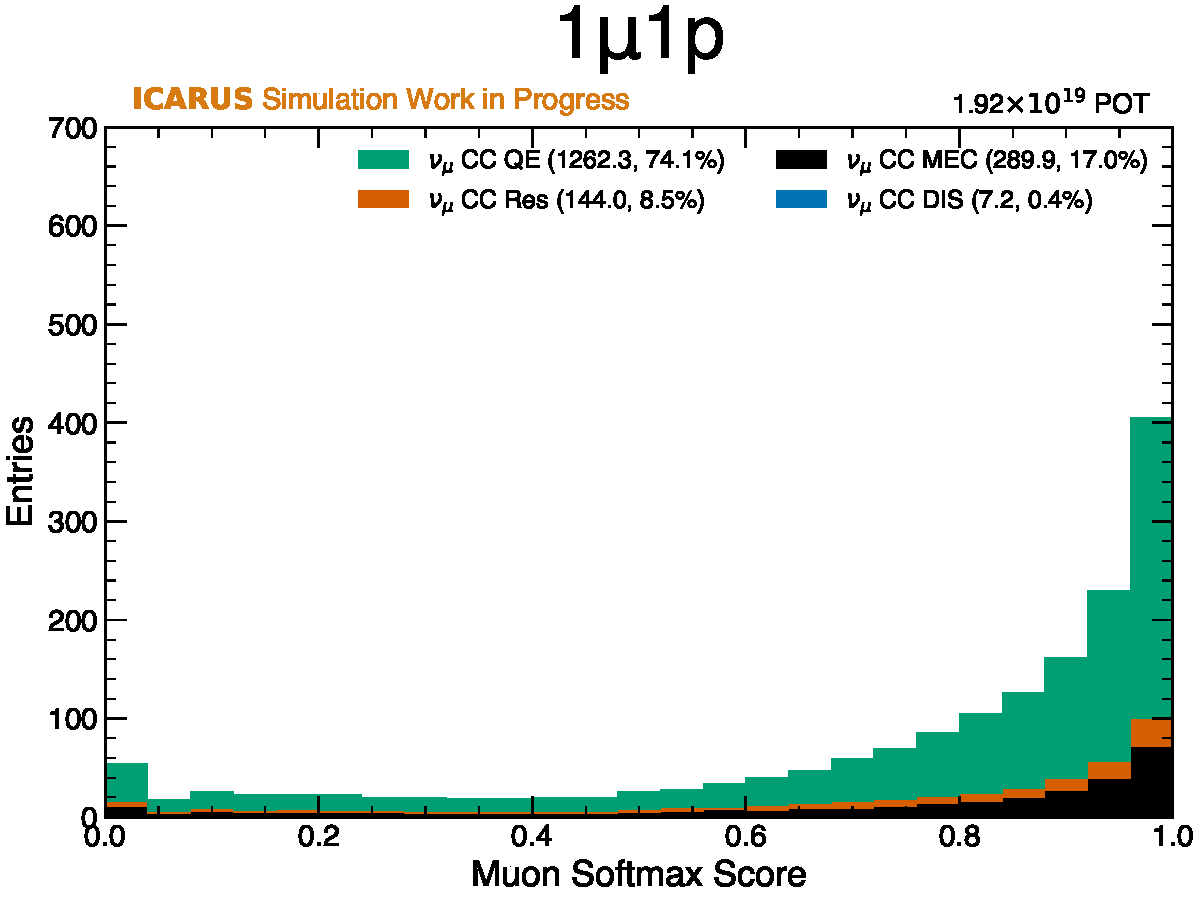
\includegraphics[width=0.48\textwidth]{figures/neutrino_selection/signal_hist1d_1mu1p_muon_softmax.pdf}
    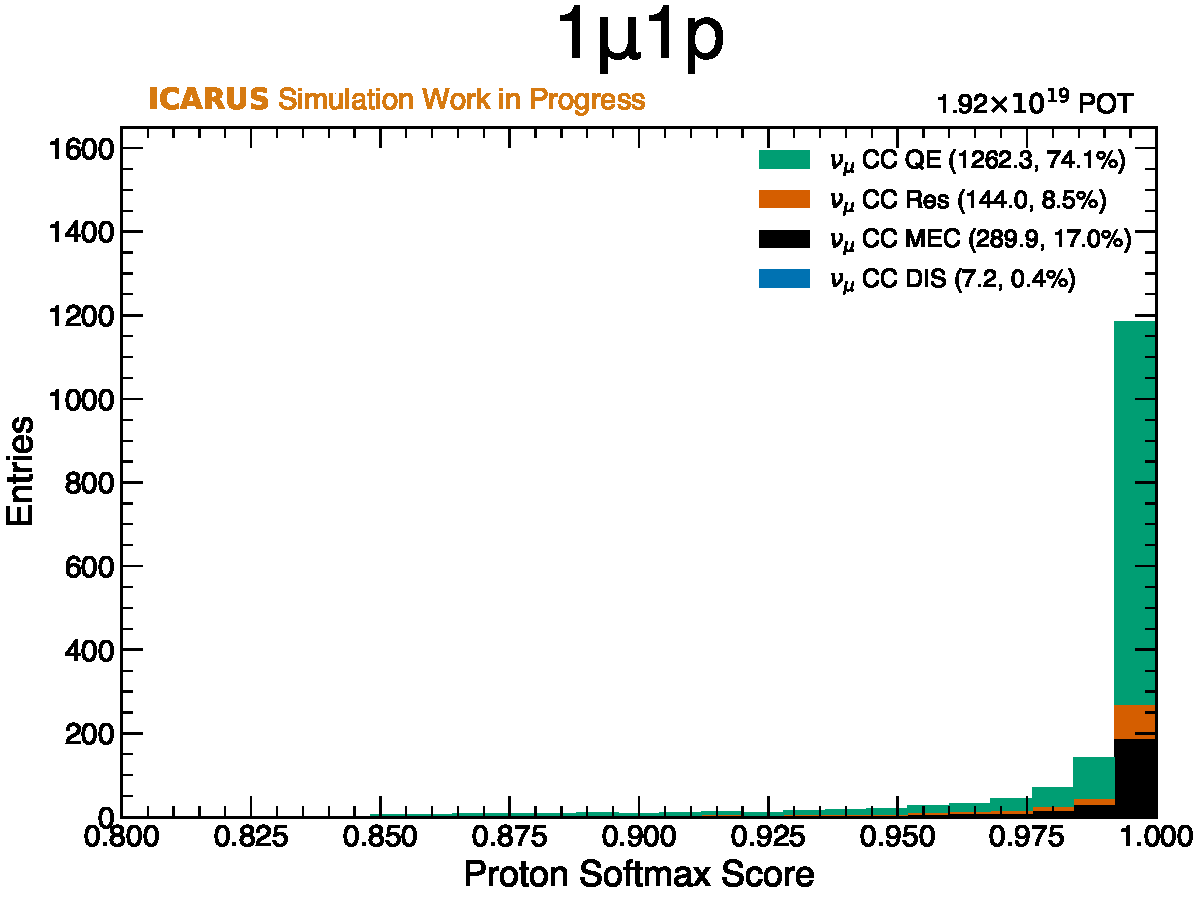
\includegraphics[width=0.48\textwidth]{figures/neutrino_selection/signal_hist1d_1mu1p_proton_softmax.pdf}
    \\
    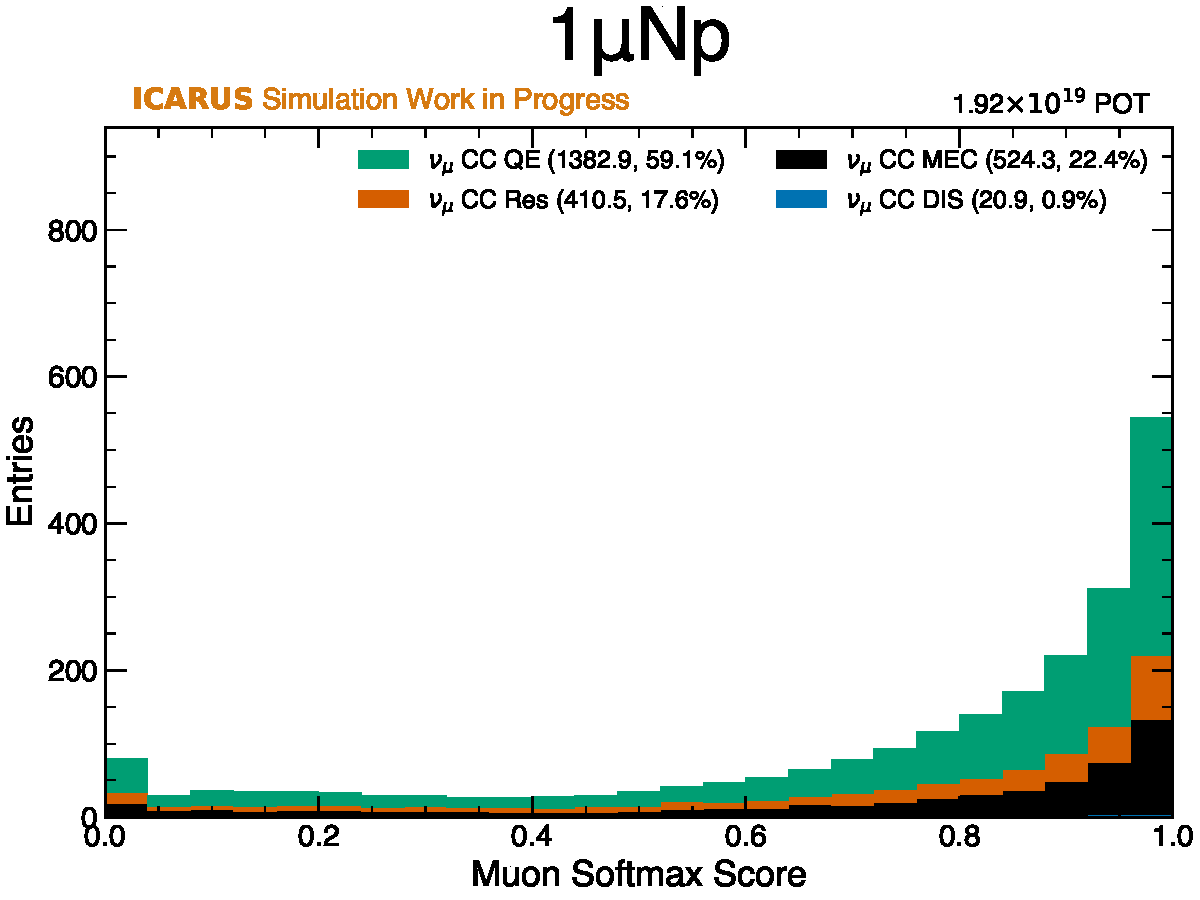
\includegraphics[width=0.48\textwidth]{figures/neutrino_selection/signal_hist1d_1muNp_muon_softmax.pdf}
    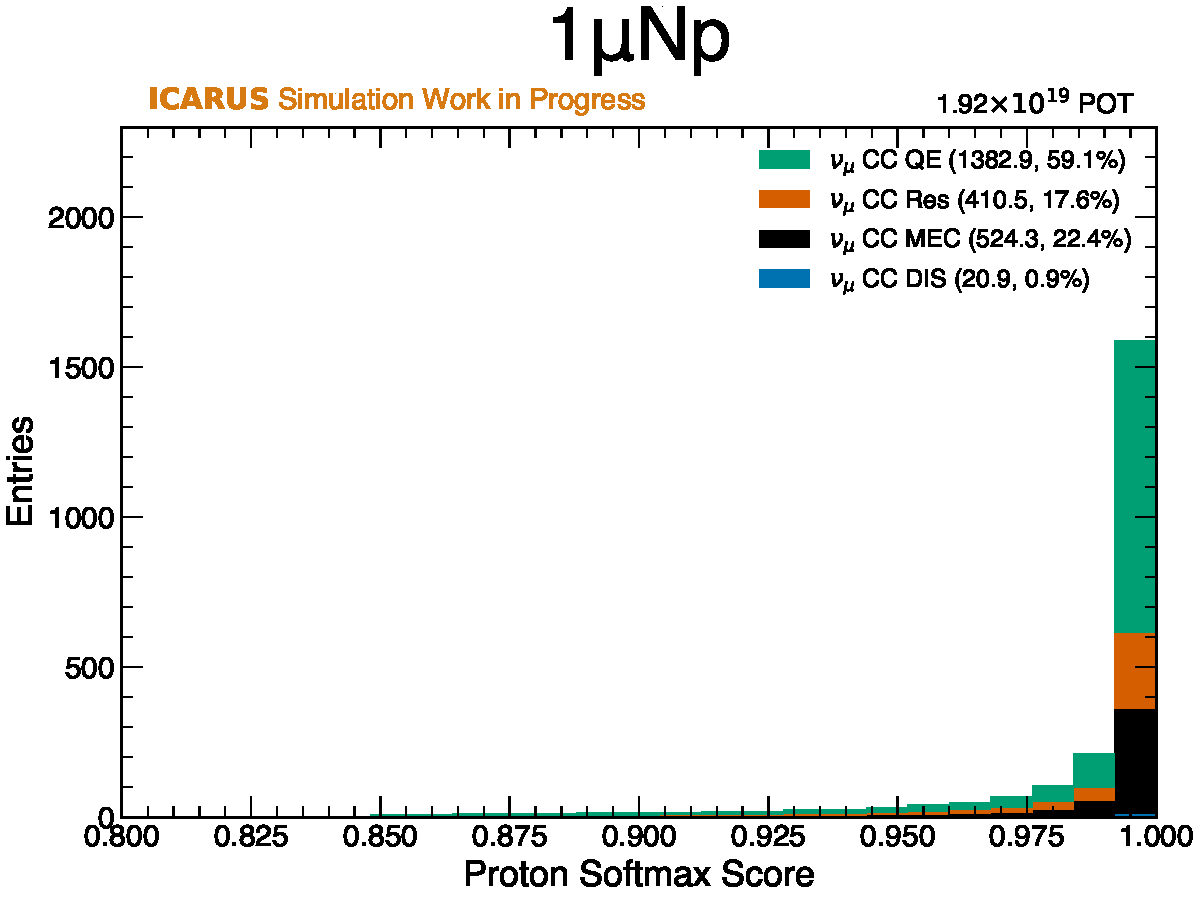
\includegraphics[width=0.48\textwidth]{figures/neutrino_selection/signal_hist1d_1muNp_proton_softmax.pdf}
    \\
    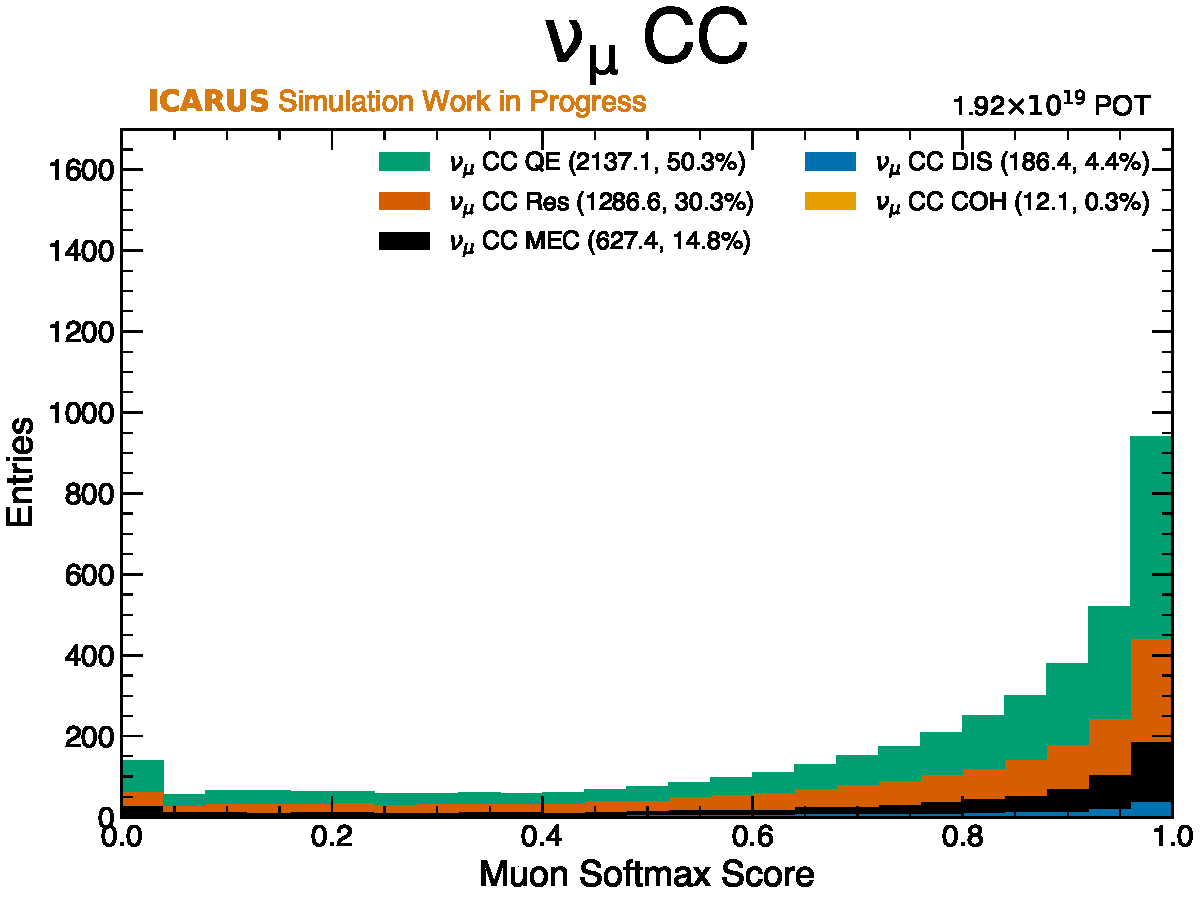
\includegraphics[width=0.48\textwidth]{figures/neutrino_selection/signal_hist1d_1muX_muon_softmax.pdf}
    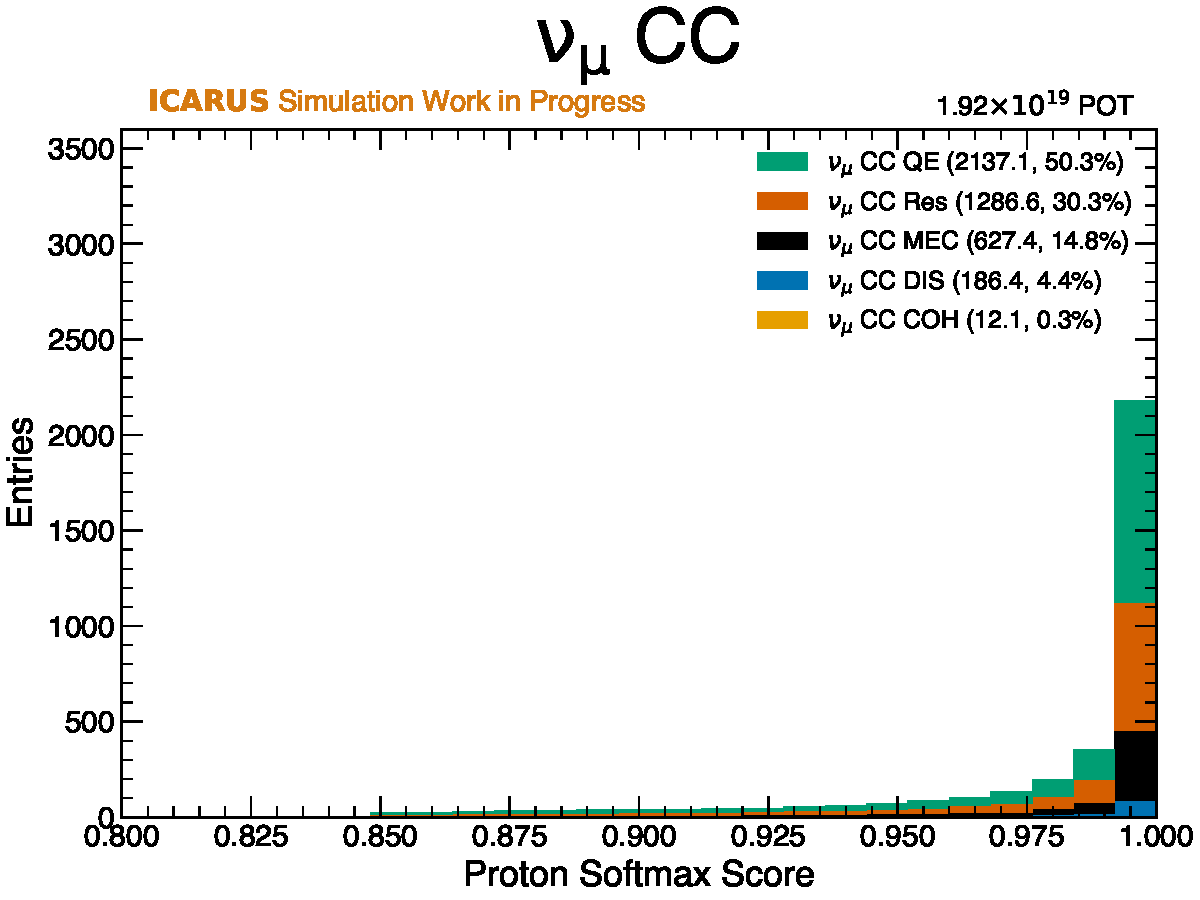
\includegraphics[width=0.48\textwidth]{figures/neutrino_selection/signal_hist1d_1muX_proton_softmax.pdf}
    \caption{Softmax PID scores for the muon candidate (left) and the leading proton candidate (right) for each of the three signal channels: from top to bottom $\mathrm{1\mu 1p}$, $\mathrm{1\mu Np}$, and $\nu_\mu$ CC inclusive.}
    \label{fig:softmax_pid}
\end{figure}

\subsection{Selection Performance}
\label{sec:selection_performance}

The performance of a selection can be characterized by its purity and efficiency. The purity of a selection is defined as the fraction of selected events that are true signal events, while the efficiency is defined as the fraction of true signal events that are selected. It is worth noting that the definition of efficiency used here is relative to the signal definition and not to the total number of neutrino interactions as may be used in other contexts. 

A table summarizing the purity and efficiency of the selections for each of the signal channels is shown in Table \ref{tab:purity_efficiency}. The purity and efficiency are calculated using the definitions described above using a Bayesian method \cite{Casadei2012} that produces more robust error bars in cases where the purity or efficiency fraction is near zero or one. Each row denotes the successive application of the selection cuts, providing a clear way to understand the impact of each cut on the purity and efficiency of the selection. From this table, several conclusions can be drawn:

\begin{table}
    \centering
    \caption{Summary of the purity and efficiency of the selections for each of the signal channels.}
    \resizebox{0.99\textwidth}{!}{\begin{tabular}{ccccccc}
\toprule
Selection Cut & $1\mu1p$ Purity [\%] & $1\mu1p$ Efficiency [\%] & $1\mu Np$ Purity [\%] & $1\mu Np$ Efficiency [\%] & $\nu_\mu$ CC Purity [\%] & $\nu_\mu$ CC Efficiency [\%] \\
\midrule
No Cut & 0.0 & 99.9 & 0.1 & 100.0 & 0.1 & 100.0 \\
Fiducial Volume & 0.1 & 98.8 & 0.1 & 98.8 & 0.3 & 98.2 \\
Containment & 1.1 & 94.9 & 1.5 & 95.0 & 3.5 & 94.1 \\
Final State & 66.2 & 73.9 & 71.2 & 77.9 & 9.5 & 86.3 \\
Flash Time & 80.1 & 72.4 & 83.0 & 76.4 & 87.8 & 84.5 \\
CRT Veto & 80.3 & 71.3 & 83.3 & 75.4 & 90.4 & 83.3 \\
\bottomrule
\end{tabular}}
    \label{tab:purity_efficiency}
\end{table}

\begin{itemize}
    \item The application of the containment cut provides a significant improvement in purity for all signal channels. This is most pronounced for the $\nu_\mu$ CC inclusive channel, where cosmic backgrounds are larger. This cut also has a non-negligible impact on the efficiency of the selection. This is largely due to cases where an un-contained cosmic-induced interaction is clustered into the neutrino interaction.
    \item The application of the cut on the final state of the candidate interactions has a significant impact on the purity of the selection for all three channels, though the impact is not as pronounced for the $\nu_\mu$ CC inclusive channel due to the presence of larger cosmic backgrounds. This is also where we see the biggest impact on the efficiency of the selection - an effect that can be directly attributed to imperfections in the reconstruction. This efficiency loss is larger for the two exclusive channels, where the final state is more constrained.
    \item The flash time cut has a negligible impact on the efficiency of the selection for all three channels, and only provides an additional improvement in purity for the $\nu_\mu$ CC inclusive channel. This is consistent with the expectation that the flash time cut primarily targets cosmic-induced interactions that are not in-time with the beam. These backgrounds are largest for the $\nu_\mu$ CC inclusive channel, which is why the impact of this cut is most pronounced for this channel.
    \item The CRT veto cut also has a $\sim$1\% impact on the efficiency of the selection for all three channels. Purity is not significantly improved except for the $\nu_\mu$ CC inclusive channel, where remaining in-time cosmic backgrounds are largest. The cost to the efficiency, though small, may not be worth it for the two exclusive channels. Since this analysis is focused on demonstrating the performance of all three selections, it is included in the final selection for all three channels to maintain consistency. It is worth highlighting that this cut may be significantly more important if the signal was extended to include interactions that exit the detector.
\end{itemize}

\begin{figure}[!htb]
    \centering
    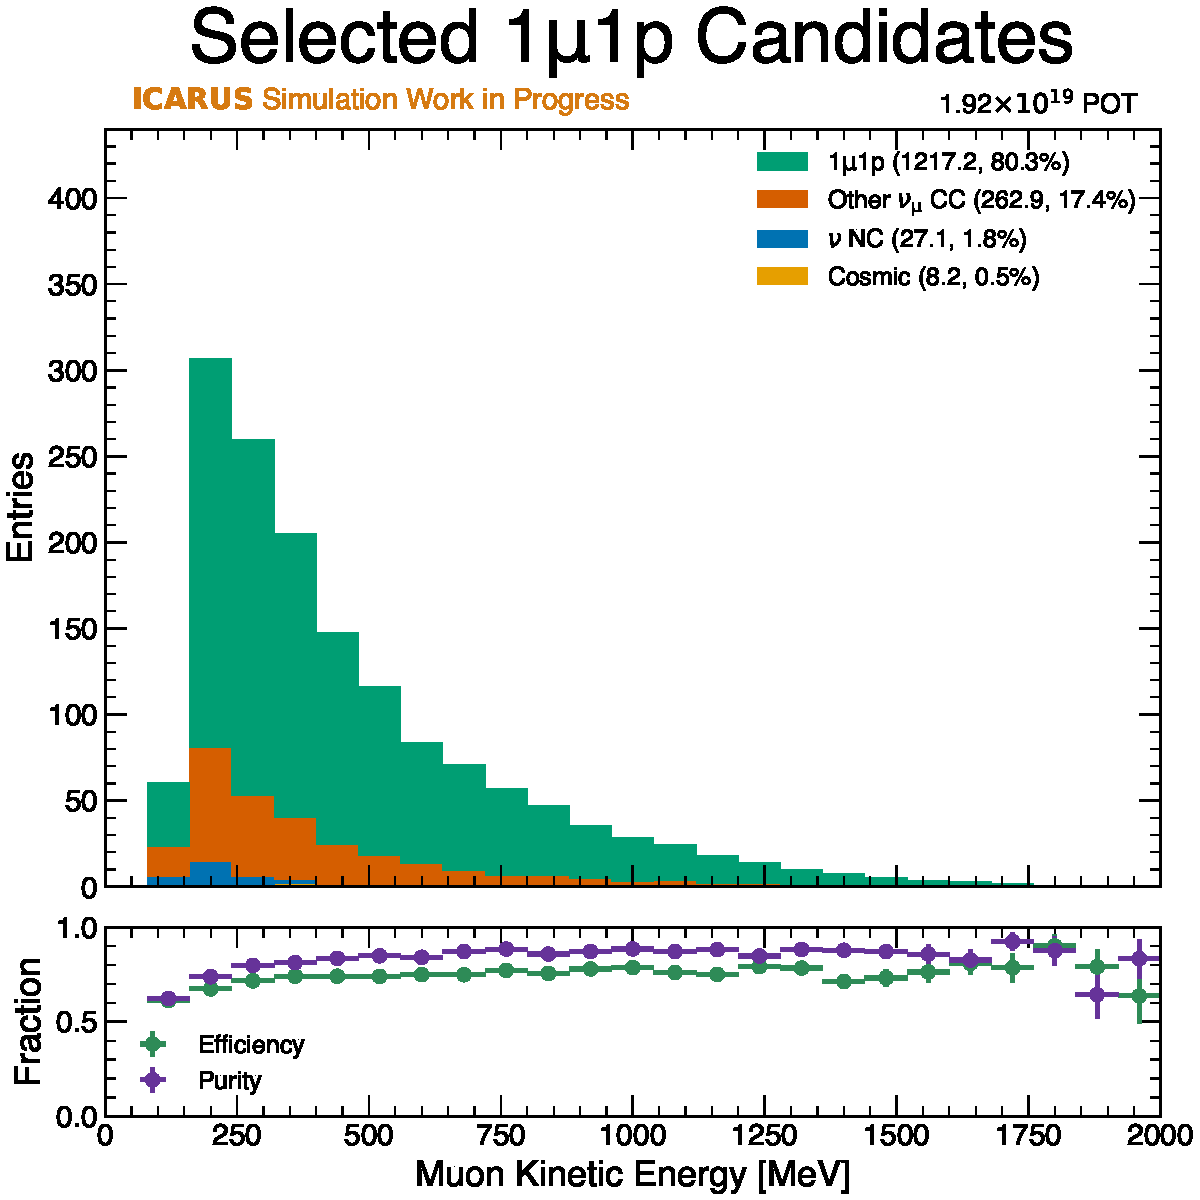
\includegraphics[width=0.42\textwidth]{figures/neutrino_selection/selected_hist1d_1mu1p_muon_ke.pdf}
    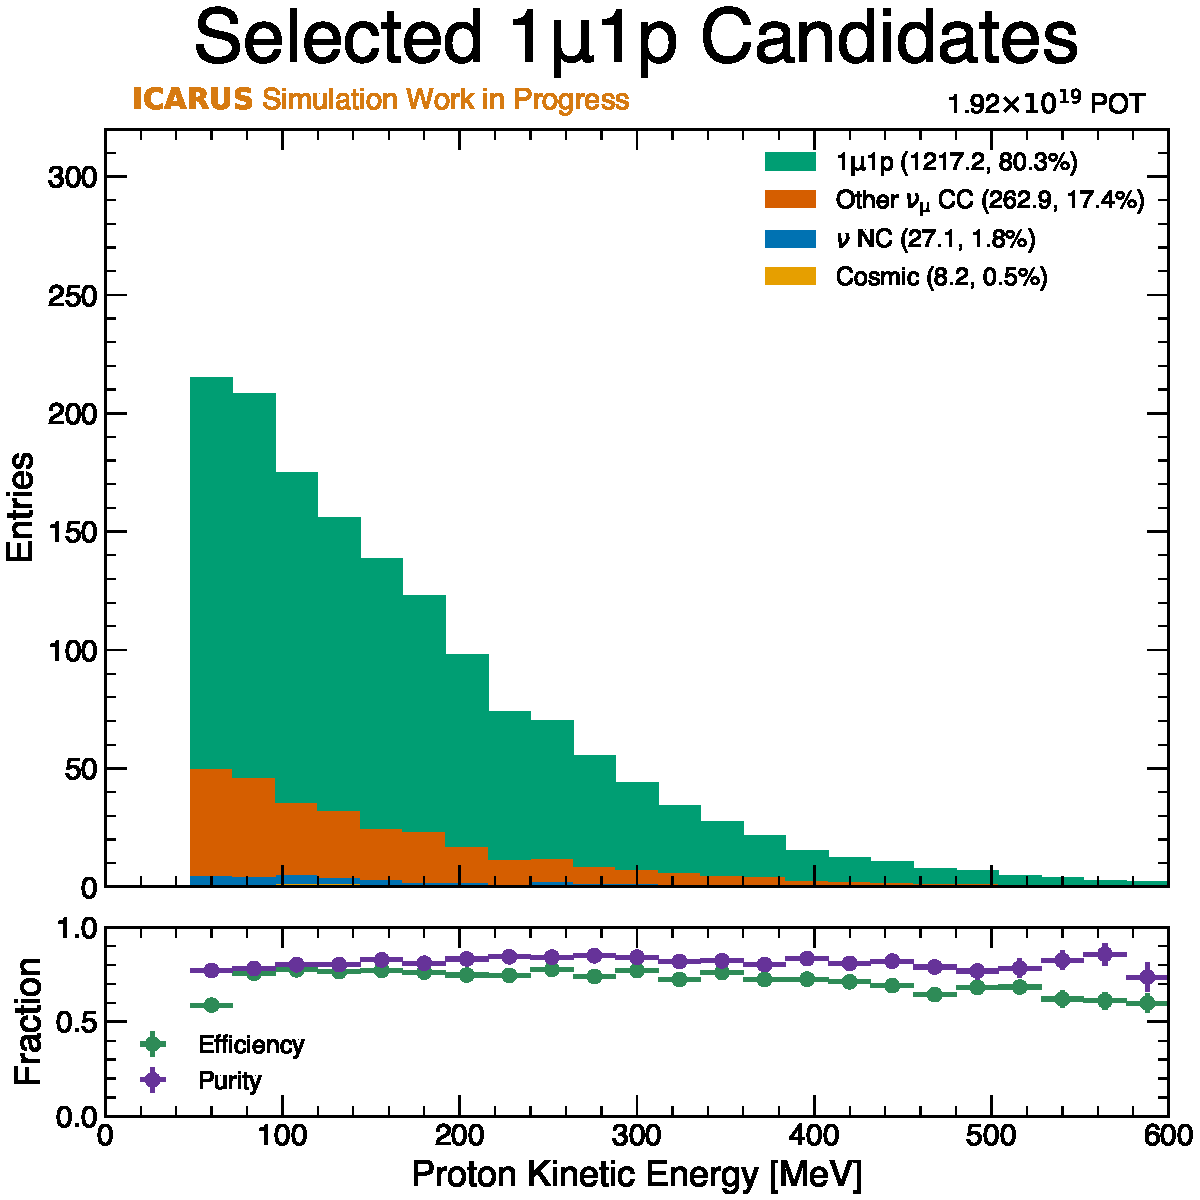
\includegraphics[width=0.42\textwidth]{figures/neutrino_selection/selected_hist1d_1mu1p_proton_ke.pdf}
    \\
    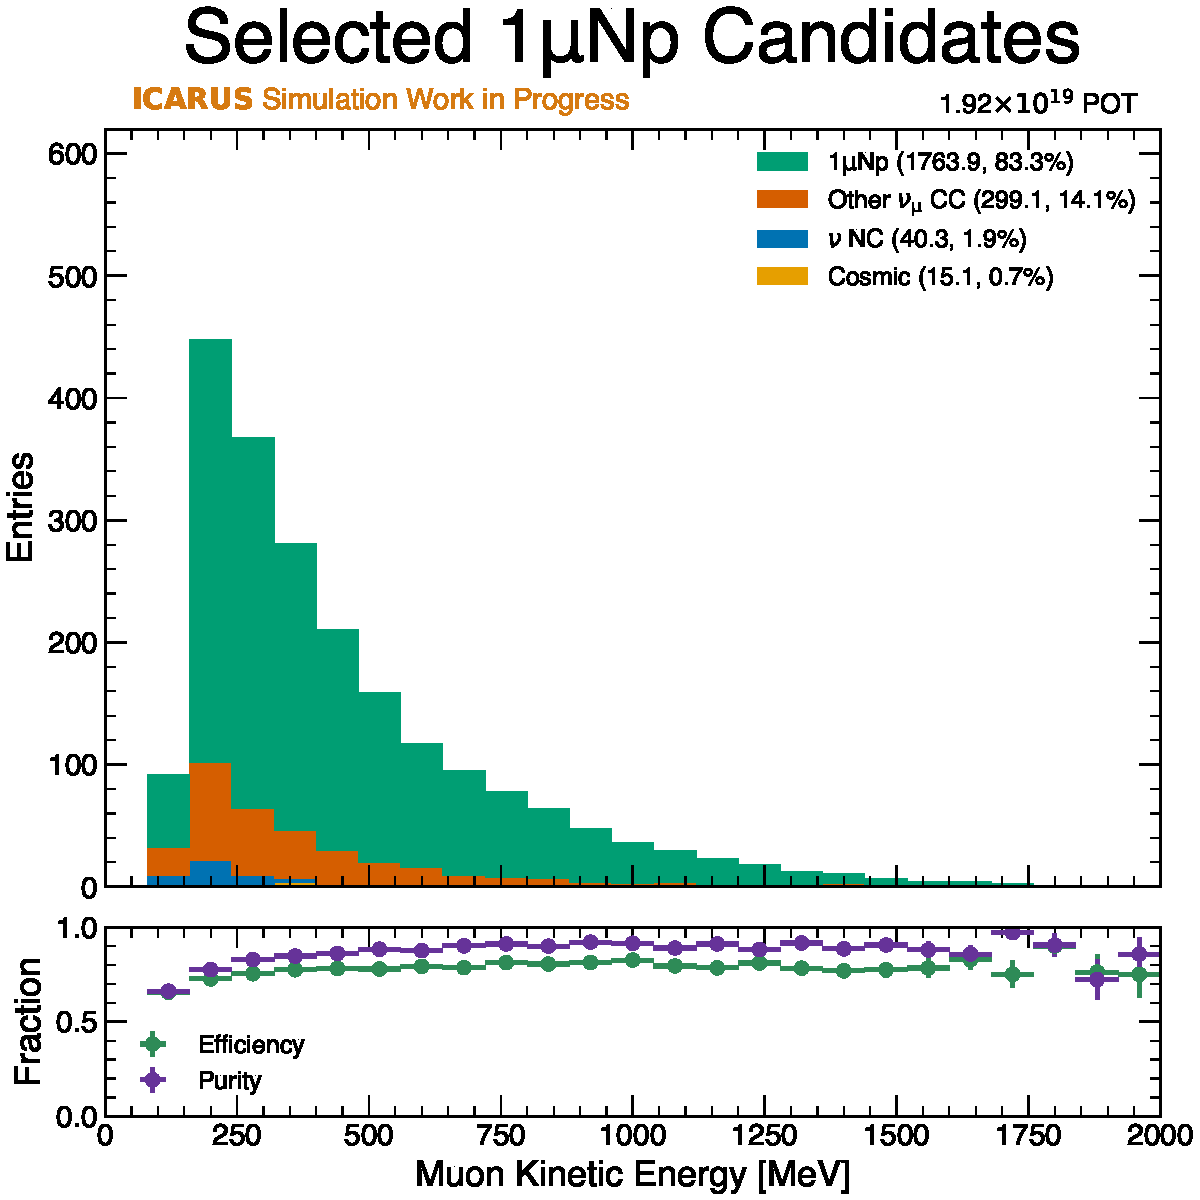
\includegraphics[width=0.42\textwidth]{figures/neutrino_selection/selected_hist1d_1muNp_muon_ke.pdf}
    \includegraphics[width=0.42\textwidth]{figures/neutrino_selection/selected_hist1d_1muNp_proton_ke.pdf}
    \\
    \includegraphics[width=0.42\textwidth]{figures/neutrino_selection/selected_hist1d_1muX_muon_ke.pdf}
    \includegraphics[width=0.42\textwidth]{figures/neutrino_selection/selected_hist1d_1muX_proton_ke.pdf}
    \caption{Purity and efficiency as a function of the kinetic energy of the muon (left) and the most energetic proton (right) for each of the three signal channels: from top to bottom $\mathrm{1\mu 1p}$, $\mathrm{1\mu Np}$, and $\nu_\mu$ CC inclusive.}
    \label{fig:pureff_muon_proton_ke}
\end{figure}

\begin{figure}[!htb]
    \centering
    \includegraphics[width=0.42\textwidth]{figures/neutrino_selection/selected_hist1d_1mu1p_visible_energy.pdf}\\
    \includegraphics[width=0.42\textwidth]{figures/neutrino_selection/selected_hist1d_1muNp_visible_energy.pdf}\\
    \includegraphics[width=0.42\textwidth]{figures/neutrino_selection/selected_hist1d_1muX_visible_energy.pdf}\\
    \caption{Purity and efficiency as a function of the total visible energy of the interaction for each of the signal channels: from top to bottom $\mathrm{1\mu 1p}$, $\mathrm{1\mu Np}$, and $\nu_\mu$ CC inclusive.}
    \label{fig:pureff_visible_energy}
\end{figure}

\begin{figure}[!htb]
    \centering
    \includegraphics[width=0.41\textwidth]{figures/neutrino_selection/selected_hist1d_1mu1p_muon_pt.pdf}
    \includegraphics[width=0.41\textwidth]{figures/neutrino_selection/selected_hist1d_1mu1p_proton_pt.pdf}
    \\
    \includegraphics[width=0.41\textwidth]{figures/neutrino_selection/selected_hist1d_1muNp_muon_pt.pdf}
    \includegraphics[width=0.41\textwidth]{figures/neutrino_selection/selected_hist1d_1muNp_proton_pt.pdf}
    \\
    \includegraphics[width=0.41\textwidth]{figures/neutrino_selection/selected_hist1d_1muX_muon_pt.pdf}
    \includegraphics[width=0.41\textwidth]{figures/neutrino_selection/selected_hist1d_1muX_proton_pt.pdf}
    \caption{Purity and efficiency as a function of the transverse momentum of the muon (left) and the most energetic proton (right) for each of the three signal channels: from top to bottom $\mathrm{1\mu 1p}$, $\mathrm{1\mu Np}$, and $\nu_\mu$ CC inclusive. The peak at the lowest bin in the inclusive channel in the proton transverse momentum variable is from interactions where no proton is present.}
    \label{fig:pureff_muon_proton_pt}
\end{figure}

\begin{figure}[!htb]
    \centering
    \includegraphics[width=0.42\textwidth]{figures/neutrino_selection/selected_hist1d_1mu1p_muon_polar_angle.pdf}
    \includegraphics[width=0.42\textwidth]{figures/neutrino_selection/selected_hist1d_1mu1p_muon_azimuthal_angle.pdf}
    \\
    \includegraphics[width=0.42\textwidth]{figures/neutrino_selection/selected_hist1d_1muNp_muon_polar_angle.pdf}
    \includegraphics[width=0.42\textwidth]{figures/neutrino_selection/selected_hist1d_1muNp_muon_azimuthal_angle.pdf}
    \\
    \includegraphics[width=0.42\textwidth]{figures/neutrino_selection/selected_hist1d_1muX_muon_polar_angle.pdf}
    \includegraphics[width=0.42\textwidth]{figures/neutrino_selection/selected_hist1d_1muX_muon_azimuthal_angle.pdf}
    \caption{Purity and efficiency as a function of the polar angle (left) and azimuthal angle (right) of the muon for each of the three signal channels: from top to bottom $\mathrm{1\mu 1p}$, $\mathrm{1\mu Np}$, and $\nu_\mu$ CC inclusive.}
    \label{fig:pureff_muon_angles}
\end{figure}

\begin{figure}[!htb]
    \centering
    \includegraphics[width=0.42\textwidth]{figures/neutrino_selection/selected_hist1d_1mu1p_opening_angle.pdf}\\
    \includegraphics[width=0.42\textwidth]{figures/neutrino_selection/selected_hist1d_1muNp_opening_angle.pdf}\\
    \includegraphics[width=0.42\textwidth]{figures/neutrino_selection/selected_hist1d_1muX_opening_angle.pdf}\\
    \caption{Purity and efficiency as a function of the the muon-proton opening angle for each of the three signal channels: from top to bottom $\mathrm{1\mu 1p}$, $\mathrm{1\mu Np}$, and $\nu_\mu$ CC inclusive.}
    \label{fig:pureff_opening_angle}
\end{figure}

\begin{figure}[!htb]
    \centering
    \includegraphics[width=0.42\textwidth]{figures/neutrino_selection/selected_hist1d_1mu1p_delta_pT.pdf}\\
    \includegraphics[width=0.42\textwidth]{figures/neutrino_selection/selected_hist1d_1muNp_delta_pT.pdf}\\
    \includegraphics[width=0.42\textwidth]{figures/neutrino_selection/selected_hist1d_1muX_delta_pT.pdf}\\
    \caption{Purity and efficiency as a function of the transverse momentum of the interaction for each of the three signal channels: from top to bottom $\mathrm{1\mu 1p}$, $\mathrm{1\mu Np}$, and $\nu_\mu$ CC inclusive.}
    \label{fig:pureff_delta_pT}
\end{figure}

\begin{figure}[!htb]
    \centering
    \includegraphics[width=0.42\textwidth]{figures/neutrino_selection/selected_hist1d_1mu1p_delta_alphaT.pdf}
    \includegraphics[width=0.42\textwidth]{figures/neutrino_selection/selected_hist1d_1mu1p_delta_phiT.pdf}
    \\
    \includegraphics[width=0.42\textwidth]{figures/neutrino_selection/selected_hist1d_1muNp_delta_alphaT.pdf}
    \includegraphics[width=0.42\textwidth]{figures/neutrino_selection/selected_hist1d_1muNp_delta_phiT.pdf}
    \\
    \includegraphics[width=0.42\textwidth]{figures/neutrino_selection/selected_hist1d_1muX_delta_alphaT.pdf}
    \includegraphics[width=0.42\textwidth]{figures/neutrino_selection/selected_hist1d_1muX_delta_phiT.pdf}
    \caption{Purity and efficiency as a function of the kinematic imbalance variables $\delta \alpha_T$ (left) and $\delta \phi_T$ (right) for each of the three signal channels: from top to bottom $\mathrm{1\mu 1p}$, $\mathrm{1\mu Np}$, and $\nu_\mu$ CC inclusive.}
    \label{fig:pureff_kinematic_imbalance_angles}
\end{figure}

The purity and efficiency of a selection can also be visualized as a function of the variables of interest to understand the relationship between the selection and each variable. This can help to identify regions of phase space where the selection is particularly efficient or pure, and to identify regions where the selection may be underperforming. In each of the following plots, the purity and efficiency are calculated per-bin using the same binning as the variable itself. The selected candidates are binned according to the \textit{reconstructed} variable, as opposed to the true quantity presented previously, and broken down into categories based on their true final state. These plots are shown in Figures \ref{fig:pureff_muon_proton_ke} through \ref{fig:pureff_kinematic_imbalance_angles}. There are several notable features worth highlighting:

\begin{itemize}
    \item Generally, the purity and efficiency drop off at regions of phase space correlated with lower energy. Smaller particles are more likely to be mis-reconstructed and may not be as separable from other particles in the final state. 
    \item Angles where tracks are parallel to the wire planes are more likely to be mis-reconstructed. This is especially visible in the muon and proton transverse momentum variables, where the lower values are associated with a particle that is more aligned with the $z$-axis. This is a known side effect of the coherent noise filtering algorithm used upstream in the reconstruction chain, which tends to remove signal from tracks that are parallel to the wire planes.
    \item There is a drop in purity and efficiency for the two exclusive channels at higher values of the muon-proton opening angle. This is due to the difficulty in separating the muon and proton tracks when they are highly collinear.
    \item The values of $\delta p_T$ outside of the Fermi momentum are associated with a drop in purity and efficiency for the two exclusive channels. This is a region of phase space with fewer QE interactions and more complex interactions that are more difficult to reconstruct.
\end{itemize}

At this stage of the analysis, the selections are performing well in terms of purity and efficiency on simulation. Benchmarking the performance of the selections on data is a key step in the validation of the selections and the reconstruction chain, but prior to this step the full set of uncertainties must be understood. This will be the focus of the next chapter.



\section{Systematic Uncertainties}
\label{chap:systematics}
Comparisons of the neutrino selection between data and Monte Carlo simulation only gain meaning within the context of properly characterized uncertainties on both the data measurement and the Monte Carlo simulation. The data measurement inherently contains statistical uncertainty reflecting the size of the data set. The expectation from the Monte Carlo simulation has, in addition to statistical uncertainty, other sources of systematic uncertainty arising from the uncertainty in the BNB flux, the neutrino interaction model, and the response of the detector to neutrino interactions.

The covariance matrix formalism \cite{Eaton2007} is used to accurately capture the scale and bin-to-bin correlations of each source of uncertainty. Under the assumption that the underlying sources of uncertainty are independent, the bilinearity of the covariance matrix allows for the independent calculation of covariance matrices for each source and the calculation of the total covariance matrix as the sum over all covariance matrices. It is worth noting that the effect of the sources of uncertainty are in general correlated to some degree, but the underlying sources are often independent. Section \ref{sec:bnb_flux} describes the estimation of uncertainties associated with the BNB flux prediction. Section \ref{sec:xsec} describes the estimation of uncertainties associated with the modeling of $\nu$-Ar interactions using the GENIE event generator. Section \ref{sec:detector_response} describes the procedure for estimating systematic uncertainties associated with the modeling of detector effects. Finally, a summary of the overall uncertainties in the analysis is presented in Section \ref{sec:uncertainty_conclusion}.

\subsection{BNB Flux Uncertainties}
\label{sec:bnb_flux}
The BNB flux prediction used for ICARUS is based on the flux prediction computed for MiniBooNE \cite{Aguilar2009}. The production rate of hadrons through $p$-Be interactions in the target is modeled using a GEANT4 simulation \cite{Agostinelli2003} and includes some additional re-weighting of pion production based on hadron production data as measured in the HARP experiment \cite{Prior2005}. In addition to the uncertainties arising from hadron production, there are also uncertainties associated with the re-scattering of pions and protons in the beryllium and aluminum horn through quasielastic and inelastic processes and the mis-modeling of current flow through the magnetic focusing horn. Additionally, there is a flat 2\% uncertainty associated with the total number of POT due to the uncertainty in the measured POT from the BNB \cite{Aguilar2009}.

The estimation of the flux covariance matrix follows a ``many-universe'' technique, where the flux parameters associated with these systematic uncertainty sources are varied following a Gaussian distribution centered at the predicted central value and width. A total of $M=1000$ universes are simulated in this way for each systematic parameter and each neutrino interaction is assigned a weight reflecting the probability of the true parameter living in that universe. After binning the selected interactions for each universe, the covariance $E_{ij}^\alpha$ between bins $i$ and $j$ under the effect of systematic parameter $\alpha$ is computed as:

\begin{equation}
    \label{eq:covariance}
    E_{ij}^{\alpha} = \frac{1}{M} \sum_{m=1}^M (N_{CV}^i - N_{\alpha, m}^i)(N_{CV}^j - N_{\alpha, m}^j)
\end{equation}

\noindent
where $N_{CV}^i$ is the central value prediction for bin $i$ and $N_{\alpha,m}^i$ is the content of bin $i$ in the universe $m$. The total covariance matrix is then computed as the sum of the covariance matrices for each systematic parameter. This process is then be repeated for each reconstructed variable discussed in Section \ref{sec:variables_of_interest}. A breakdown of the flux uncertainty is shown in Table \ref{tab:flux}.

\begin{table}
    \centering
    \caption{A breakdown of the overall scale of each flux uncertainty for each of the three signal definitions. Beamline uncertainties are those associated with the re-scattering of hadrons in the target and the modeling of the magnetic focusing horn. Hadron production uncertainties are those associated with the production of hadrons in the target.}
    \begin{tabular}{ccccc}
\toprule
Uncertainty & Type & $1\mu1p$ [\%] & $1\mu Np$ [\%] & $\nu_\mu$ CC [\%] \\
\midrule
Skin Depth & Beamline & 2.2 & 2.7 & 3.2 \\
Horn Current & Beamline & 0.4 & 0.5 & 0.5 \\
$\pi^+$ & Hadron Production & 4.7 & 4.7 & 4.8 \\
$\pi^-$ & Hadron Production & 0.1 & 0.0 & 0.1 \\
$K^+$ & Hadron Production & 0.1 & 0.1 & 0.2 \\
$K^-$ & Hadron Production & 0.0 & 0.0 & 0.0 \\
$K^0_L$ & Hadron Production & 0.0 & 0.0 & 0.0 \\
Nucleon Inelastic & Beamline & 0.9 & 0.9 & 0.9 \\
Nucleon QE & Beamline & 2.5 & 2.5 & 2.5 \\
Nucleon Total & Beamline & 0.8 & 0.8 & 0.8 \\
$\pi$ Inelastic & Beamline & 1.2 & 1.2 & 1.2 \\
$\pi$ QE & Beamline & 0.8 & 0.9 & 0.8 \\
$\pi$ Total & Beamline & 0.7 & 0.8 & 0.8 \\
POT & Beamline & 2.0 & 2.0 & 2.0 \\
\midrule
Total Flux &  & 6.7 & 6.9 & 7.3 \\
\bottomrule
\end{tabular}
    \label{tab:flux} 
\end{table}

\subsection{Neutrino Interaction Uncertainties}
\label{sec:xsec}

Neutrino interactions are simulated using the GENIE event generator \cite{Andreopoulos2015} for the central value prediction. Within GENIE, there are a large number of parameters available for re-weighting that are used in the simulation of neutrino interactions. To estimate the uncertainty in the neutrino interaction model, the many-universe technique is used to vary these parameters in order to individually characterize their effect on the downstream analysis. The covariance matrix for each parameter is computed with Equation \ref{eq:covariance} as done for the flux uncertainties. The total covariance matrix is then computed as the sum of the covariance matrices for each parameter. A breakdown of the neutrino interaction model uncertainty is shown in Table \ref{tab:xsec}.

\begin{table}
    \centering
    \caption{A breakdown of the overall scale of each neutrino interaction model uncertainty for each of the three signal definitions.}
    \resizebox{0.99\textwidth}{!}{\begin{tabular}{ccccc}
\toprule
Uncertainty & Description & $1\mu1p$ [\%] & $1\mu Np$ [\%] & $\nu_\mu$ CC [\%] \\
\midrule
ZExpAVariationResponse & Z-expansion description of the axial-vector form factor on CC-QE & 9.6 & 8.1 & 6.3 \\
RPA CCQE & RPA suppression of CC-QE & 4.7 & 3.3 & 6.8 \\
Coulomb CCQE & The strength of the electromagnetic potential for the Coulomb corrections on CC-QE & 0.5 & 0.4 & 0.3 \\
Norm CCMEC & Normalization of CC-MEC & 7.5 & 10.2 & 7.1 \\
Norm NCMEC & Normalization of NC-MEC & 0.0 & 0.0 & 0.0 \\
NCEL Variation Response & Variation of the dipole form factor on NCEL & 0.1 & 0.1 & 0.1 \\
CCRES Variation Response & Variation of the dipole form factor on CC-RES & 2.2 & 4.5 & 6.7 \\
NCRES Variation Response & Variation of the dipole form factor on NC-RES & 0.4 & 0.4 & 0.5 \\
NonRESBGvpCC1pi & Scale factor for the non-resonant background level of $\nu$-p CC + 1$\pi$ & 0.0 & 0.1 & 0.1 \\
NonRESBGvpCC2pi & Scale factor for the non-resonant background level of $\nu$-p CC + 2$\pi$ & 0.1 & 0.2 & 0.6 \\
NonRESBGvpNC1pi & Scale factor for the non-resonant background level of $\nu$-p NC + 1$\pi$ & 0.0 & 0.0 & 0.0 \\
NonRESBGvpNC2pi & Scale factor for the non-resonant background level of $\nu$-p NC + 2$\pi$ & 0.0 & 0.0 & 0.1 \\
NonRESBGvnCC1pi & Scale factor for the non-resonant background level of $\nu$-n CC + 1$\pi$ & 0.1 & 0.2 & 0.4 \\
NonRESBGvnCC2pi & Scale factor for the non-resonant background level of $\nu$-n CC + 2$\pi$ & 0.1 & 0.2 & 0.7 \\
NonRESBGvnNC1pi & Scale factor for the non-resonant background level of $\nu$-n NC + 1$\pi$ & 0.2 & 0.2 & 0.2 \\
NonRESBGvnNC2pi & Scale factor for the non-resonant background level of $\nu$-n NC + 2$\pi$ & 0.0 & 0.0 & 0.0 \\
NonRESBGvbarpCC1pi & Scale factor for the non-resonant background level of $\bar{\nu}$-p CC + 1$\pi$ & 0.0 & 0.0 & 0.0 \\
NonRESBGvbarpCC2pi & Scale factor for the non-resonant background level of $\bar{\nu}$-p CC + 2$\pi$ & 0.0 & 0.0 & 0.0 \\
NonRESBGvbarpNC1pi & Scale factor for the non-resonant background level of $\bar{\nu}$-p NC + 1$\pi$ & 0.0 & 0.0 & 0.0 \\
NonRESBGvbarpNC2pi & Scale factor for the non-resonant background level of $\bar{\nu}$-p NC + 2$\pi$ & 0.0 & 0.0 & 0.0 \\
NonRESBGvbarnCC1pi & Scale factor for the non-resonant background level of $\bar{\nu}$-n CC + 1$\pi$ & 0.0 & 0.0 & 0.0 \\
NonRESBGvbarnCC2pi & Scale factor for the non-resonant background level of $\bar{\nu}$-n CC + 2$\pi$ & 0.0 & 0.0 & 0.0 \\
NonRESBGvbarnNC1pi & Scale factor for the non-resonant background level of $\bar{\nu}$-n NC + 1$\pi$ & 0.0 & 0.0 & 0.0 \\
NonRESBGvbarnNC2pi & Scale factor for the non-resonant background level of $\bar{\nu}$-n NC + 2$\pi$ & 0.0 & 0.0 & 0.0 \\
RDecBR1gamma & Scale factor for the branching fraction of X + 1$\gamma$ & 0.0 & 0.0 & 0.0 \\
RDecBR1eta & Scale factor for the branching fraction of X + 1$\eta$ & 0.2 & 0.3 & 0.4 \\
COH Variation Response & Normalization of the Coherent production process & 0.1 & 0.1 & 0.2 \\
DISBY Variation Response & Normalization of the BY model of the DIS process & 0.0 & 0.0 & 0.0 \\
FSI $\pi$ Variation Response & Variation for FSI involving pions & 1.2 & 3.5 & 0.7 \\
FSI N Variation Response & Variation for FSI involving nucleons & 3.9 & 3.0 & 1.2 \\
\midrule
Total Cross Section &  & 14.7 & 15.7 & 14.6 \\
\bottomrule
\end{tabular}}
    \label{tab:xsec}
\end{table}

Many of these individual parameters have a small effect on the overall uncertainty, but there are a few worth highlighting:

\begin{itemize}
    \item The parameter associated with the Z-expansion of the axial form factor has a large effect on the overall uncertainty. This is especially true for the two exclusive channels, which are more dominated by QE interaction modes.
    \item The RPA suppression parameter has an effect in the range of 3-7\%. This is largest for the inclusive channel.
    \item The normalization for CC MEC processes is large for all channels, but is especially large for the 1$\mu$N$p$ channel. This is due to the larger contribution of MEC processes to the 1$\mu$N$p$ channel.
    \item The parameter controlling the dipole form factor for CC resonant production is progressively larger as the final state becomes less restrictive due to higher contributions from resonant production.
    \item Many of the parameters associated with anti-neutrino interactions have vanishingly small effects on the overall uncertainty. This is due to the low flux of anti-neutrinos in the BNB in the ``neutrino-mode'' horn configuration, which has been the operating mode for all physics datasets collected by the ICARUS detector.
\end{itemize}

Overall, all three channels have a resulting total uncertainty due to interaction model uncertainties of around 15\%. The 1$\mu$N$p$ channel has a slightly larger uncertainty (around 1\% more) due to the larger contribution of MEC processes to this channel, which have larger uncertainties associated with them.

\subsection{Detector Response Uncertainties}
\label{sec:detector_response}
The detector response uncertainty reflects many non-idealizations of the ICARUS detector and the underlying detector physics that can impact event reconstruction and signal selection. The effects considered can be broadly grouped into three categories:

\begin{enumerate}
    \item Light yield, scintillation photon propagation, and optical response throughout the detector.
    \item Electron-ion recombination, space charge effects, electron lifetime, diffusion, and other processes affecting drifting ionization charge.
    \item Variable TPC channel gain, non-uniformities in response across the wire planes, electronic noise, and other effects impacting signal reconstruction associated with the TPC wires.
\end{enumerate}

The detector response uncertainty is characterized through dedicated detector variation samples. Each detector variation sample implements a single variation in some underlying component of the Monte Carlo simulation that fully covers some aspect of the detector response that is not fully understood or known to be insufficiently modeled. 

A sample of $N_{CV}$ total events generated with the nominal simulation parameters and run through the full detector simulation and event reconstruction is used as the central value prediction. The same set of $N_{CV}$ events is then run through the full detector simulation and event reconstruction with the detector variation applied. Random processes in the GEANT4 simulation of particle trajectories and secondaries may produce additional statistical differences between the nominal and systematic variation sample, so a workflow which shares the generated particles and their trajectories between both samples is used to characterize the detector systematics. A diagram representing the full simulation chain for both the nominal simulation and a detector variation sample is shown in Figure \ref{fig:systematic_variation_sample_flow}.

\begin{figure}
    \centering
    \includegraphics[width=0.95\textwidth]{figures/systematics/systematic_variation_sample_flow.png}
    \caption{A diagram representing the full simulation chain for both the nominal simulation (green) and a detector variation sample (gold). The samples share the same set of generated events including particle trajectories and daughters, but downstream processes may vary according to statistical processes or the variation itself.}
    \label{fig:systematic_variation_sample_flow}
\end{figure}

For this analysis, samples of $N_{CV} = 200,000$ events were generated for the central value and each detector variation sample. The choice of detector systematics to vary was made based on the expected impact of the variation on the final event selection. This list is not exhaustive and further detector systematics will be studied in the future. Due to the large time and computational resources required to generate each sample, the decision was made to use neutrino-only samples to characterize the detector systematics. Though the presence of cosmic rays does have an impact on the selection, the relative effect of the variation on the selection is expected to be similar between the neutrino-only and full samples. The detector variation samples produced for this analysis are:

\paragraph{TPC Signal Shape:}
This is a variation in the shape of the signal response on the wire planes. The central value sample uses a signal response that was tuned with cosmic muon data, whereas the variation sample uses the original signal response that was produced with a simulation. This is a conservative estimate of the uncertainty in the signal shape, as this is essentially treating the full effect of a known bias as a systematic uncertainty. Future detector systematic studies within ICARUS will aim to better characterize the uncertainty in the signal shape.

\paragraph{First Induction Plane Gain:}
This is a variation in the gain of the first induction plane of $\pm 15\%$, implemented separately as two distinct samples. These variations reflect the un-simulated variation of the gain across the first induction plane.

\paragraph{PMT Quantum Efficiency:}
There is a known data to simulation discrepancy in the optical model that is in the process of being understood. This variation is meant to cover this discrepancy by varying the quantum efficiency of the PMTs by $4\%$. In addition to potential impacts on the flash matching performance, this variation also directly impacts the emulated trigger decision and therefore may cause a shift in the selected events by changing the trigger efficiency.

\paragraph{TPC Coherent Noise:}
The coherent component of the TPC noise varied by $4.9\%$ with respect to the nominal noise model over the duration of Run 2. A positive variation of this scale is applied to the nominal simulation to cover this discrepancy.

\paragraph{TPC Intrinsic Noise:}
Similar to the coherent noise variation, the intrinsic noise of the TPC varied by $3.7\%$ with respect to the nominal noise model over the duration of Run 2. A positive variation of this scale is applied to the nominal simulation to cover this discrepancy.

\paragraph{Electron-ion Recombination:}
The recombination model used in the nominal simulation is the Modified Box model, as measured by ArgoNeuT \cite{Acciarri2013}. Recently, the dependence of recombination on the angle of the track with respect to the electric field has been measured at ICARUS and encapsulated in a model referred to as the ``Ellipsoidal'' recombination model. The variation sample uses this model to estimate the uncertainty that may arise from improperly modeling recombination.

\vspace{\baselineskip}
The comparison of the central value and variation samples is used to estimate the uncertainty in the detector response. The procedure used is covered in the following section.

\subsubsection{Bootstrapping}
\label{sec:bootstrapping}

The detector response uncertainty is estimated using a bootstrapping technique similar to the one employed in several differential cross section measurements performed by the MicroBooNE collaboration \cite{Abratenko2022f,Abratenko2022e,Abratenko2024}. An overview of bootstrapping techniques can be found in \cite{Chernick2011}. The general idea is to estimate the uncertainty in a measurement by repeatedly sampling the data with replacement and computing the quantity of interest for each sample. The distribution of these quantities is then used to estimate the uncertainty in the measurement. This method inherently captures the bin-to-bin correlations in the uncertainty, which is important for the downstream analysis. The assumption made in this method is that the distribution being sampled from is sufficiently large enough to represent the true distribution of the data.

In the bootstrapping technique used for this analysis, the set of common events between the central value and a variation sample is sampled $N_{CV}$ times with replacement to form one ``universe.'' In each universe, the selected signal candidates from the central value sample and the variation sample are binned according to the reconstructed variable of interest. A difference vector $\vec{V}_{D,i}$ is computed for the $i$'th universe as the difference across the bins between the two samples. This process is repeated $N_{\text{bootstrap}} = 1000$ times to form a distribution of difference vectors. The average $1\sigma$ deviation $\vec{V}^{nominal}_D$ is then computed as the average of the difference vectors across the universes.

The uncertainty on $\vec{V}^{nominal}_D$ is then computed as the covariance matrix $M_R$ of the difference vectors across the universes as is described in Equation \ref{eq:covariance}. This covariance matrix can be understood as the matrix governing the Gaussian distribution of the difference vectors, or in other words the matrix that describes how to perturb $\vec{V}^{nominal}_D$ according to the fluctuations seen in the bootstrapping procedure.

The overall covariance matrix for the variation is then computed using both $\vec{V}^{nominal}_D$ and $M_R$ in a way that fully captures the detector response uncertainty. A new set of universes is generated in this step, with $N_{\text{universes}} = 1000$. In each universe, the matrix $M_R$ is used to generate a perturbation $\delta \vec{V}_D$ by sampling from a Gaussian distribution centered at $\vec{V}^{nominal}_D$ with covariance $M_R$. This is realized by computing the Cholesky decomposition of $M_R$ and using this to generate a random vector with elements correlated according to $M_R$ from a vector with normally distributed, uncorrelated elements. The perturbation $\delta \vec{V}_D$ is then added to the central value vector $\vec{V}^{nominal}$ and scaled by a unit Gaussian $r_i$ to form the final vector $\vec{V}^{final}_D$, as shown in Equation \ref{eq:final_vector}.

\begin{equation}
    \label{eq:final_vector}
    \vec{V}^{final}_{D,i} = r_i \left(\vec{V}^{nominal} + \delta \vec{V}_{D,i}\right)
\end{equation}

\noindent
This set of vectors $\vec{V}^{final}_{D,i}\ \forall i \in [1, N_{\text{universes}}]$ is then used to compute the covariance matrix $M_D$ that describes the uncertainty on the event selection due to the variation in the detector response. This process is then repeated for each of the variation samples and for each of the reconstructed variables discussed in Section \ref{sec:variables_of_interest}. These covariance matrices can then be combined to form the total covariance matrix for the detector response uncertainty. A breakdown of the detector response uncertainty is shown in Table \ref{tab:detector_systematics}

\begin{table}
    \centering
    \caption{A breakdown of the overall scale of each detector response uncertainty for each of the three signal definitions.}
    \begin{tabular}{ccccc}
\toprule
Uncertainty & Type & $1\mu1p$ [\%] & $1\mu Np$ [\%] & $\nu_\mu$ CC [\%] \\
\midrule
TPC Signal Shape & TPC & 5.5 & 6.4 & 3.3 \\
Increased Front Induction Gain & TPC & 2.1 & 2.2 & 2.2 \\
Decreased Front Induction Gain & TPC & 2.3 & 2.2 & 2.4 \\
Ellipsoidal Recombination & TPC & 2.1 & 1.9 & 2.5 \\
Increased Coherent Noise & TPC & 2.1 & 2.2 & 2.2 \\
Increased Intrinsic Noise & TPC & 2.5 & 2.3 & 2.4 \\
PMT Quantum Efficiency & PMT & 2.1 & 2.2 & 2.2 \\
\midrule
Total Detector &  & 8.1 & 8.6 & 6.9 \\
\bottomrule
\end{tabular}
    \label{tab:detector_systematics}
\end{table}

From these results, it is clear that the variation of the TPC signal shape is the most impactful on this analysis. This is not surprising as the signal shape is a fundamental aspect of the signal processing and affects all downstream reconstruction. Additionally, as noted in the summary of the variations above, this variation treats the full effect of a known bias as a systematic uncertainty. Work is ongoing within ICARUS to establish post-calibration uncertainties to more accurately model this effect. In contrast, the other variations have reached a floor of around 2\% uncertainty. A few things are likely contributing to this floor: the statistical nature of the bootstrapping technique, the size of the sample used to estimate the uncertainty, and the remaining statistical processes that are not fully shared between the central value and variation samples. The actual uncertainty due to these variations is likely smaller than the 2\% floor, so the TPC signal shape uncertainty can be treated as lower bound on the uncertainty due to the detector response.

\subsubsection{Summary of Event Selection Uncertainties}
\label{sec:uncertainty_conclusion}

The overall uncertainty in the event selection is computed as the sum of the covariance matrices for each source of uncertainty described in the previous sections. This total covariance matrix can then be used to place uncertainty bars on the histogram entries for each reconstructed variable used in the analysis, thus allowing for a visual representation of the uncertainty in the event selection. A more quantitative use of the covariance matrix is in the calculation of the $\chi^2$ test statistic between data and the prediction. This will be discussed in more detail in the next chapter. A summary of the overall uncertainty in the event selection, broken down by category, is shown in Table \ref{tab:overall_systematics}. The total correlation matrix for the 1$\mu$1$p$, 1$\mu$N$p$, and $\nu_\mu$ CC inclusive channels is shown in Figure \ref{fig:correlation_matrices}.

\begin{table}
    \centering
    \caption{A breakdown of the overall scale of each uncertainty source by category for each of the three signal definitions.}
    \resizebox{0.99\textwidth}{!}{\begin{tabular}{cp{8cm}ccc}
\toprule
Uncertainty & Description & $1\mu1p$ [\%] & $1\mu Np$ [\%] & $\nu_\mu$ CC [\%] \\
\midrule
Detector & Uncertainties related to the modeling of the detector response & 8.1 & 8.6 & 6.9 \\
Flux & Uncertainties related to the modeling of the neutrino flux & 6.7 & 6.9 & 7.3 \\
Cross Section & Uncertainties related to neutrino interaction modeling & 14.7 & 15.7 & 14.6 \\
Statistical & Statistical uncertainties associated with the Monte Carlo simulation sample & 2.4 & 2.0 & 1.6 \\
Off-beam Statistical & Statistical uncertainties associated with the off-beam sample used to estimate cosmic backgrounds & 0.3 & 0.4 & 0.5 \\
\midrule
Total &  & 18.6 & 19.6 & 18.3 \\
\bottomrule
\end{tabular}}
    \label{tab:overall_systematics}
\end{table}

\begin{figure}
    \centering
    \includegraphics[width=0.55\textwidth]{figures/systematics/correlations_1mu1p.pdf} \\
    \includegraphics[width=0.55\textwidth]{figures/systematics/correlations_1muNp.pdf} \\
    \includegraphics[width=0.55\textwidth]{figures/systematics/correlations_1muX.pdf} \\
    \caption{The total correlation matrix for the 1$\mu$1$p$ (top), 1$\mu$N$p$ (middle), and $\nu_\mu$ CC inclusive (bottom) channels. The variable shown is the reconstructed visible energy.}
    \label{fig:correlation_matrices}
\end{figure}

By far the largest source of uncertainty in the event selection is the neutrino interaction model uncertainty. This will have the biggest impact in ICARUS-only analyses, where cancellation of systematic uncertainties between the near and far detectors is not possible. The detector response uncertainty is the next largest source of uncertainty, but is expected to be reduced in future analyses as the detector response simulation is improved and more precise variations of the detector response are implemented. Looking towards joint SBN analyses where the flux and neutrino interaction model uncertainties cancel to first order, the detector response uncertainty will become the dominant source of uncertainty. The statistical uncertainty associated with the simulated central value sample and the off-beam dataset are both negligible in comparison to the other sources of uncertainty.

\section{Data/Simulation Comparisons}
\label{chap:data_mc_comparisons}
This chapter presents a comparison of Run 2 ICARUS data and the corresponding expectations from simulation. Section \ref{sec:run2_dataset} describes the dataset used for this analysis, including the rejection of subsets of the dataset due to non-ideal detector conditions and the steps taken to comply with the ICARUS blinding policy. Section \ref{sec:data_comparisons} presents the comparison of data and simulation in each of the reconstructed variables along with some discussion on the observed data/simulation agreement. 


\subsection{Run 2 Dataset}
\label{sec:run2_dataset}

The dataset used for this analysis consists of the ICARUS Run 2 data collected between December 20, 2022 and July 16, 2023. This period of data collection represents the largest dataset with stable detector conditions collected by the ICARUS T600 detector at Fermilab to date, corresponding to approximately $2.05 \times 10^{20}$ POT.

\subsubsection{Data Quality}
\label{sec:data_quality}

Though the detector was overall stable throughout the duration of this physics run, there were instances of detector instabilities that resulted in portions of DAQ runs being flagged as bad. These instabilities were typically due to single-component failures, such as the power supply of a TPC readout crate, or due to issues with the DAQ, trigger, cathode, or wire bias systems. These issues were logged and used as part of the data processing to identify and remove bad runs from the dataset. This results in a final dataset of around $1.92 \times 10^{20}$ POT.

\subsubsection{The ICARUS Blinding Policy}
\label{sec:blinding_policy}

The ICARUS collaboration has an official data blinding policy in place to prevent experimenter bias in the analysis of the data. The philosophy behind this policy is to ensure that an analyzer will not prematurely access the data in a statistically significant way that could influence the development of the analysis. By default, only $10\%$ of the data is fully unblinded for the purpose of developing the analysis, while the remaining $90\%$ is kept blinded until the analysis is finalized. The blinding policy also sets a process for accessing the blinded data, which is typically done in stages following the submission of technical documentation of the analysis and review by the collaboration. 

In practical terms, this policy is enforced at the level of the ICARUS data processing and analysis software. A decision is made per-event to determine if the event is blinded or unblinded using a random number service that is seeded with a configurable parameter. This allows for reproducible blinding decisions, which is important for maintaining the same set of blinded events across all data-processing campaigns. The files (``Common Analysis Framework'' files, or CAF files) containing analysis-level information for the $10\%$ of the data that is declared unblinded are kept entirely separate from the CAF files containing the blinded data. It is worth noting that this policy only applies to data streams that contain neutrino interactions and not to cosmic-only data streams such as the off-beam data.

The goals of this analysis are to demonstrate the performance of the ICARUS machine-learning analysis chain on the Run 2 dataset in signal channels of relevance for ICARUS and the SBN Program. This can be done with the $10\%$ of the data that is unblinded and does not require the increased statistics of the full Run 2 dataset. The final dataset size for this analysis is therefore $1.92 \times 10^{19}$ POT, after accounting for data processing inefficiencies and removing data from periods of detector instability. The data used for this analysis was processed in full compliance with the ICARUS blinding policy. At no point during the development of this analysis was any portion of the blinded data accessed. 

\subsection{Data/Simulation Comparisons}
\label{sec:data_comparisons}
This section presents the comparison of Run 2 ICARUS data and the corresponding expectations from simulation across a wide range of variables. The comparison is performed for the three signal channels of interest for ICARUS and the SBN Program: $\mathrm{1\mu 1p}$, $\mathrm{1\mu Np}$, and $\nu_\mu$ CC inclusive. Agreement between data and simulation is crucial for demonstrating the readiness of the ICARUS machine-learning analysis chain for future analyses. 

Each of the subsections below shows a set of distributions for a particular set of variables. In each distribution, the data is shown as black points with error bars representing the statistical uncertainty on the data. The expectation from the combination of simulation and off-beam data is shown as the filled histogram, with the error bands representing the full uncertainty as described in Chapter \ref{chap:systematics}. The lower panel of each plot shows the ratio of data to the expectation with the same error bars and bands superimposed.

To quantitatively assess the agreement, the $\chi^2$ test statistic is calculated for each distribution. The $\chi^2$ is calculated using the sum of the overall covariance matrix for the expectation and the statistical covariance matrix for the data:

\begin{equation}
    \chi^2 = \sum_{i,j} \left( O_i - E_i \right) \left( \Sigma^{-1} \right)_{ij} \left( O_j - E_j \right)
\end{equation}

\noindent
where $O_i$ and $E_i$ are the observed and expected values in bin $i$, respectively, and $\Sigma$ is the covariance matrix. The $\chi^2$ is then normalized by the number of degrees of freedom, which is the number of nonzero bins minus one. The $\chi^2$ per degree of freedom is reported for each distribution.

\subsubsection{Comparisons for Interaction Kinematic Variables}
\label{sec:datamc_interaction_kinematic_variables}

\begin{figure}
    \centering
    \includegraphics[width=0.42\textwidth]{figures/data_mc_comparisons/datamc_hist1d_1mu1p_muon_ke.pdf}
    \includegraphics[width=0.42\textwidth]{figures/data_mc_comparisons/datamc_hist1d_1mu1p_proton_ke.pdf}
    \\
    \includegraphics[width=0.42\textwidth]{figures/data_mc_comparisons/datamc_hist1d_1muNp_muon_ke.pdf}
    \includegraphics[width=0.42\textwidth]{figures/data_mc_comparisons/datamc_hist1d_1muNp_proton_ke.pdf}
    \\
    \includegraphics[width=0.42\textwidth]{figures/data_mc_comparisons/datamc_hist1d_1muX_muon_ke.pdf}
    \includegraphics[width=0.42\textwidth]{figures/data_mc_comparisons/datamc_hist1d_1muX_proton_ke.pdf}
    \caption{Comparison of data and simulation for the kinetic energy of the muon (left) and the most energetic proton (right) for each of the three signal channels: from top to bottom $\mathrm{1\mu 1p}$, $\mathrm{1\mu Np}$, and $\nu_\mu$ CC inclusive.}
    \label{fig:datamc_muon_proton_ke}
\end{figure}

\begin{figure}
    \centering
    \includegraphics[width=0.42\textwidth]{figures/data_mc_comparisons/datamc_hist1d_1mu1p_visible_energy.pdf}\\
    \includegraphics[width=0.42\textwidth]{figures/data_mc_comparisons/datamc_hist1d_1muNp_visible_energy.pdf}\\
    \includegraphics[width=0.42\textwidth]{figures/data_mc_comparisons/datamc_hist1d_1muX_visible_energy.pdf}\\
    \caption{Comparison of data and simulation for the total visible energy of the interaction for each of the signal channels: from top to bottom $\mathrm{1\mu 1p}$, $\mathrm{1\mu Np}$, and $\nu_\mu$ CC inclusive.}
    \label{fig:datamc_visible_energy}
\end{figure}

\begin{figure}
    \centering
    \includegraphics[width=0.41\textwidth]{figures/data_mc_comparisons/datamc_hist1d_1mu1p_muon_pt.pdf}
    \includegraphics[width=0.41\textwidth]{figures/data_mc_comparisons/datamc_hist1d_1mu1p_proton_pt.pdf}
    \\
    \includegraphics[width=0.41\textwidth]{figures/data_mc_comparisons/datamc_hist1d_1muNp_muon_pt.pdf}
    \includegraphics[width=0.41\textwidth]{figures/data_mc_comparisons/datamc_hist1d_1muNp_proton_pt.pdf}
    \\
    \includegraphics[width=0.41\textwidth]{figures/data_mc_comparisons/datamc_hist1d_1muX_muon_pt.pdf}
    \includegraphics[width=0.41\textwidth]{figures/data_mc_comparisons/datamc_hist1d_1muX_proton_pt.pdf}
    \caption{Comparison of data and simulation for the transverse momentum of the muon (left) and the most energetic proton (right) for each of the three signal channels: from top to bottom $\mathrm{1\mu 1p}$, $\mathrm{1\mu Np}$, and $\nu_\mu$ CC inclusive. The peak in the lowest bin of the proton transverse momentum distribution in the inclusive channel is from interactions that do not have a proton in the final state.}
    \label{fig:datamc_muon_proton_pt}
\end{figure}

\begin{figure}
    \centering
    \includegraphics[width=0.42\textwidth]{figures/data_mc_comparisons/datamc_hist1d_1mu1p_muon_polar_angle.pdf}
    \includegraphics[width=0.42\textwidth]{figures/data_mc_comparisons/datamc_hist1d_1mu1p_muon_azimuthal_angle.pdf}
    \\
    \includegraphics[width=0.42\textwidth]{figures/data_mc_comparisons/datamc_hist1d_1muNp_muon_polar_angle.pdf}
    \includegraphics[width=0.42\textwidth]{figures/data_mc_comparisons/datamc_hist1d_1muNp_muon_azimuthal_angle.pdf}
    \\
    \includegraphics[width=0.42\textwidth]{figures/data_mc_comparisons/datamc_hist1d_1muX_muon_polar_angle.pdf}
    \includegraphics[width=0.42\textwidth]{figures/data_mc_comparisons/datamc_hist1d_1muX_muon_azimuthal_angle.pdf}
    \caption{Comparison of data and simulation for the polar angle (left) and azimuthal angle (right) of the muon for each of the three signal channels: from top to bottom $\mathrm{1\mu 1p}$, $\mathrm{1\mu Np}$, and $\nu_\mu$ CC inclusive.}
    \label{fig:datamc_muon_angles}
\end{figure}

Comparisons of data and simulation are presented in Figures \ref{fig:datamc_muon_proton_ke} through \ref{fig:datamc_muon_angles} for the interaction kinematic variables defined in Section \ref{sec:interaction_kinematic_variables}. Generally, an excess of events is observed in the data compared to simulation, but the difference is near the expected uncertainty. The muon and proton energy distributions seem to have shifts in the distribution that are opposite: the muon energy distribution is shifted to higher energies in data compared to simulation, while the proton energy distribution is shifted to lower energies. The total visible energy distribution shows a generally higher amount of events in data compared to simulation, but the shape of the distribution matches well.

There are no significant deviations in the muon and proton transverse momentum distributions, the muon polar and azimuthal angle distributions, or the muon-proton opening angle distributions. Many reconstruction inefficiencies, such as signal removal from coherent noise filtering, could potentially impact these distributions, so it is especially important that we see good agreement in these variables. 

\subsubsection{Comparisons for Kinematic Imbalance Variables}
\label{sec:datamc_kinematic_imbalance_variables}

\begin{figure}
    \centering
    \includegraphics[width=0.41\textwidth]{figures/data_mc_comparisons/datamc_hist1d_1mu1p_opening_angle.pdf}\\
    \includegraphics[width=0.41\textwidth]{figures/data_mc_comparisons/datamc_hist1d_1muNp_opening_angle.pdf}\\
    \includegraphics[width=0.41\textwidth]{figures/data_mc_comparisons/datamc_hist1d_1muX_opening_angle.pdf}\\
    \caption{Comparison of data and simulation for the the muon-proton opening angle for each of the three signal channels: from top to bottom $\mathrm{1\mu 1p}$, $\mathrm{1\mu Np}$, and $\nu_\mu$ CC inclusive. The peak in the lowest bin of the proton transverse momentum distribution in the inclusive channel is from interactions that do not have a proton in the final state.}
    \label{fig:datamc_opening_angle}
\end{figure}

\begin{figure}
    \centering
    \includegraphics[width=0.42\textwidth]{figures/data_mc_comparisons/datamc_hist1d_1mu1p_delta_pT.pdf}\\
    \includegraphics[width=0.42\textwidth]{figures/data_mc_comparisons/datamc_hist1d_1muNp_delta_pT.pdf}\\
    \includegraphics[width=0.42\textwidth]{figures/data_mc_comparisons/datamc_hist1d_1muX_delta_pT.pdf}\\
    \caption{Comparison of data and simulation for the transverse momentum of the interaction for each of the three signal channels: from top to bottom $\mathrm{1\mu 1p}$, $\mathrm{1\mu Np}$, and $\nu_\mu$ CC inclusive.}
    \label{fig:datamc_delta_pT}
\end{figure}

\begin{figure}
    \centering
    \includegraphics[width=0.42\textwidth]{figures/data_mc_comparisons/datamc_hist1d_1mu1p_delta_alphaT.pdf}
    \includegraphics[width=0.42\textwidth]{figures/data_mc_comparisons/datamc_hist1d_1mu1p_delta_phiT.pdf}
    \\
    \includegraphics[width=0.42\textwidth]{figures/data_mc_comparisons/datamc_hist1d_1muNp_delta_alphaT.pdf}
    \includegraphics[width=0.42\textwidth]{figures/data_mc_comparisons/datamc_hist1d_1muNp_delta_phiT.pdf}
    \\
    \includegraphics[width=0.42\textwidth]{figures/data_mc_comparisons/datamc_hist1d_1muX_delta_alphaT.pdf}
    \includegraphics[width=0.42\textwidth]{figures/data_mc_comparisons/datamc_hist1d_1muX_delta_phiT.pdf}
    \caption{Comparison of data and simulation for the kinematic imbalance variables $\delta \alpha_T$ (left) and $\delta \phi_T$ (right) for each of the three signal channels: from top to bottom $\mathrm{1\mu 1p}$, $\mathrm{1\mu Np}$, and $\nu_\mu$ CC inclusive.}
    \label{fig:datamc_kinematic_imbalance_angles}
\end{figure}

The kinematic imbalance variables $\delta p_T$, $\alpha_T$, and $\phi_T$ are shown in Figures \ref{fig:datamc_delta_pT} and \ref{fig:datamc_kinematic_imbalance_angles}. These variables are commonly incorporated into cross section measurements, so it is important for any future ICARUS cross section measurements that the data and simulation do not show major biases in these variables. The discrepancy in these variables seem to be only a normalization offset, with the shape of the distributions matching well. These variables are also sensitive to smearing from poor angular reconstruction, so the agreement in these variables is a good indication that the angular reconstruction is working similarly in data and simulation.

\subsubsection{Comparisons for PID Variables}
\label{sec:datamc_pid_variables}

\begin{figure}[!htb]
    \centering
    \includegraphics[width=0.42\textwidth]{figures/data_mc_comparisons/datamc_hist1d_1mu1p_muon_softmax.pdf}
    \includegraphics[width=0.42\textwidth]{figures/data_mc_comparisons/datamc_hist1d_1mu1p_proton_softmax.pdf}
    \\
    \includegraphics[width=0.42\textwidth]{figures/data_mc_comparisons/datamc_hist1d_1muNp_muon_softmax.pdf}
    \includegraphics[width=0.42\textwidth]{figures/data_mc_comparisons/datamc_hist1d_1muNp_proton_softmax.pdf}
    \\
    \includegraphics[width=0.42\textwidth]{figures/data_mc_comparisons/datamc_hist1d_1muX_muon_softmax.pdf}
    \includegraphics[width=0.42\textwidth]{figures/data_mc_comparisons/datamc_hist1d_1muX_proton_softmax.pdf}
    \caption{Comparison of data and simulation for the softmax PID scores for the muon candidate (left) and the leading proton candidate (right) for each of the three signal channels: from top to bottom $\mathrm{1\mu 1p}$, $\mathrm{1\mu Np}$, and $\nu_\mu$ CC inclusive.}
    \label{fig:datamc_softmax_pid}
\end{figure}

The PID variables are shown in Figure \ref{fig:datamc_softmax_pid}. These variables, perhaps more than any of the others, are where one would expect to see efficiency differences between data and simulation. If the PID scores are not well modeled, then it is possible that data and simulation may select interactions at different rates. There is largely good agreement in the proton PID score distributions, with only an overall normalization offset manifesting in the last bin. It is clear that the data and simulation are both confident that the leading proton candidate is a proton and to similar degrees.

The muon PID score shows a significant shift of the population from the peak to lower scores in data compared to simulation. Perhaps fortuitously, the cut placed on the muon PID score is quite low at $0.1$, so this shift does not appear to affect the selection efficiency. Regardless, this discrepancy must be understood and will be the subject of upcoming investigations. One hypothesis is that the usage of the plane-averaged charge rather than collection-only charge in the space points may be introducing a smearing effect in data that is not present in simulation. The switch to collection-only charge in the space points will require re-training the network and re-running the analysis, but it is a necessary step to understand this discrepancy. Another possible source of this discrepancy is the different value of the electron lifetime used in the Monte Carlo simulation compared to the value observed in data. This will also be the subject of future investigations.



\section{Conclusions}
\label{chap:conclusion}
The analysis presented here has investigated the performance of the end-to-end machine learning reconstruction chain for the ICARUS T600 detector in three different muon neutrino signal channels: a 1$\mu$1$p$ channel, a 1$\mu$N$p$ channel, and an inclusive $\nu_\mu$ CC channel. The first two exclusive channels are most relevant for the near-term single-detector analysis goals of ICARUS, while the inclusive channel is a more general test of the performance of the machine learning chain and a target for the SBN-wide joint oscillation analysis envisioned in the SBN proposal \cite{Acciarri2015}. 

The performance of the selections in the three signal channels is quantified in terms of purity and efficiency. This analysis has demonstrated that the selections in the two exclusive channels have achieved a purity of at least 80\% and an efficiency of at least 70\% with all relevant backgrounds included. The inclusive channel has achieved a purity of 90\% and an efficiency of 83\%. In all cases, cosmic backgrounds are subdominant to mis-reconstructed neutrino backgrounds and the selections have achieved exceptional purity and efficiency. Given the 80\% efficiency for automated reconstruction outlined in the SBN proposal, this analysis has demonstrated that ICARUS meets one of its core deliverables for the joint SBN analysis. Although the full joint SBN analysis includes both contained and exiting events, this analysis can be easily extended to exiting events and is a crucial step towards the ultimate goal. Of particular note on this topic is the fact that this reconstruction has been implemented for SBND as well, meaning that this reconstruction chain has no technical hurdles for use in the joint SBN analysis.

Detector systematics have been characterized in this analysis by producing simulation samples that implement single variations in the underlying parameters controlling the detector simulation. This analysis has shown that the only significant detector systematic among those studied is the systematic associated with the TPC signal response shape on the waveforms. Though this variation is expected to be conservative, more work is required within the ICARUS collaboration to more precisely characterize and mitigate detector systematics in order to reach 2-3\% systematic uncertainty from the detector model assumed in the SBN proposal. The current level of detector systematics is not expected to be a limiting factor in ICARUS-only analyses as the neutrino interaction model dominates the systematic uncertainty in the selection.

Agreement between data and simulation is generally good across variables that probe a wide region of phase space. Two notable exceptions are the overall higher number of candidate interactions selected in data with respect to the simulation and the disagreement observed in the muon PID score variable. The former disagreement is not well-correlated with any particular distribution and is currently thought to be a result of the chosen central value parameters used in the neutrino interaction model. The ICARUS collaboration is exploring a tune of the central value parameters to better match external data. The latter disagreement may be due to the use of plane-averaged charge rather than collection-only charge, thus causing a bias in data with respect to simulation. Moreover, the electron lifetime in the Monte Carlo simulation is different from the value observed in data and may contribute to this discrepancy. This is actively being investigated at the time of writing. Overall, there are no substantial disagreements between data and simulation that would suggest an inefficiency in the selection that is correlated with a particular variable.

In conclusion, this analysis has demonstrated that the ICARUS T600 detector is capable of achieving high purity and efficiency in the selection of contained muon neutrino interactions using an end-to-end machine learning reconstruction chain. This analysis meets the deliverables outlined in the SBN proposal for the BNB muon neutrino disappearance channel of the joint oscillation analysis, and can be readily extended to the NuMI beam at ICARUS and to the SBND detector. The inclusion of un-contained muon neutrino interactions in the selection to increase statistics is a natural extension of this analysis and is a target for future work. Work is also ongoing to develop analyses with this reconstruction chain targeting electron neutrinos from the BNB and the NuMI beam. This analysis represents a critical step forward in achieving the ultimate goal of the SBN Program: a joint oscillation analysis that combines the precise reconstruction and selection of muon neutrino and electron neutrino interactions from the BNB and NuMI beams at ICARUS and the BNB at SBND. The ICARUS collaboration is well-positioned to contribute to this goal with the work presented in this technical note.

% Bibliography
%%%%%%%%%%%%%%%%%%%%%%%%%%%%%%%%%%%%%%%%%%%%%%%%%%%%%%%%%%%%%%%%

\bibliographystyle{lunsrt}
\bibliography{bibliography}

\appendix

\end{document}